% Chapter 3

\chapter{A Convex Formulation for Multi-Task Learning} % Write in your own chapter title
\label{Chapter4}
\lhead{Chapter \ref{Chapter4}. 
\emph{A Convex Formulation for Multi-Task Learning}} % Write in your own chapter title to set the page header

{\bf \small{

}}

\section{Introduction}
% Multi-Task Learning paradigms can be divided in: Feature-Based, Parameter-Based, Joint-Learning
As we have seen in Chapter~\ref{Chapter3}, the MTL proposals can be categorized in feature-based, parameter-based and combination-based approaches. Feature-based proposals have the strategy of finding a shared representation of the original features that is benefitial for all tasks. Parameter-based strategies typically use multi-task regularization schemes that, using specific regularizers, push together the parameters of the task-specialized models.
Finally, the combination-based strategies combine a common model and a task-specific one. 
%
In this chapter we will present a convex formulation for combination-based MTL. With this formulation, a general task-specialized model is defined as
\begin{equation}
    \label{eq:convexmtl_general}
    \begin{aligned}
        h_r(\cdot)
       = \lambda_r g(\cdot) + (1 - \lambda_r) g_r(\cdot) .
    \end{aligned}    
\end{equation}
Here, we use the hyperparameters $\lambda_r \in [0, 1]$ to combine in a convex way the common part $g(\cdot)$ and specific parts $g_r(\cdot)$. This general formulation is very flexible, because we can use any family of functions to model $g(\cdot)$ or $g_r(\cdot)$. It is also easily interpretable, since $\lambda_r=1$ for all $r=1, \ldots, \ntasks$ results in a common model and $\lambda_r=0$ in independent models for each task. All the values $\lambda_r \in (0, 1)$ correspond to pure MTL models, being more common when $\lambda_r$ is close to $1$ and more specific when $\lambda_r$ is close to $0$.
%
Given an MTL sample 
$$\bsample = \bigcup_{r=1}^\ntasks \{(x_1^r, y_1^r), \ldots, (x_{\npertask}^r, y_{\npertask}^r)\},$$
the MTL regularized risk functional that corresponds to this convex formulation is 
\begin{equation}
    \label{eq:convexmtl_general_regrisk}
    \risk_{\bsample} ({g, g_1, \ldots, g_\ntasks}) \defeq \sum_{r=1}^{\ntasks} \sum_{i=1}^{\npertask_r} \lossf(\lambda_r g(x_i^r) + (1 - \lambda_r) g_r(x_i^r), y_i^r) + \mu \left(\Omega(g) + \sum_{r=1}^\ntasks \Omega_r(g_r)\right) ,
\end{equation}
where $\Omega(g)$ and $\Omega_r(g_r)$ are the regularizers for the common and $r$-th task parts, respectively. Observe that, since the regularization is made independently for each part, no multi-task specific regularization scheme is needed. The task coupling is made directly in the definition of the model, which combines common and specific part, and the risk $\risk_{\bsample}$ is optimized jointly in all parts.
This has some advantages, like the preservation of convexity in the risk minimization problem or an optimization procedure that requires only slight modifications to the standard one. In this chapter these characteristics will be presented in specific models using this convex MTL formulation.
%
More specifically, it is shown how this formulation can be applied to two of the most popular model families: kernel methods, in Section~\ref{sec:convexmlt_kernel}, and neural networks, in Section~\ref{sec:convexmlt_network}.
Then, in Section~\ref{sec:convexmlt_renewable} a real-world application of the convex MTL to the prediction of renewable energy is presented.
%




\section{Convex Multi-Task Learning with Kernel Methods}\label{sec:convexmlt_kernel}
% Kernel Models are powerful: Kernel trick, high dimensionality representation
As explained in the previous chapters, kernel models offer many good properties such as an implicit transformation to a possibly infinite-dimensional space and the convexity of the problems that have to be solved for the training process. With these models a regularized risk problem is solved.
% General formulation for a kernel model
A general formulation of a training problem for kernel models is 
\begin{equation}
    \label{eq:regrisk_kernel}
    \emprisk({w}) \defeq \sum_{i=1}^{\nsamples} \lossf({w}^\intercal {\phi(\fv{x}_i)} + b, y_i) + \mu \Omega({w}) ,
\end{equation}
where $\sample$ is the sample $\{(x_1, y_1), \ldots, (x_\nsamples, y_\nsamples)\}$ and $\Omega(w)$ is a regularizer for ${w}$, typically the $L_2$ norm: $\norm{w}^2$. Observe that $b$, the bias term, is not regularized since it does not affect the capacity of the hypothesis space.
In~\eqref{eq:regrisk_kernel} $\phi$ is a fixed transformation function such that there exists a ``kernel trick'', that is a kernel function $k$ for which
\begin{equation}
    \nonumber
    \dotp{\phi(x)}{\phi(y)} = k(x, y).
\end{equation}
That is, $\phi$ is an element of \acrshort{rkhs}, where $k$ is the reproducing kernel. 
The Representer Theorem~\citep*{ScholkopfHS01} states that the optimal solution of problem~\eqref{eq:regrisk_kernel} has the following form
\begin{equation}
    \nonumber
    w^* = \sum_{i=1}^\nsamples \alpha_i \phi(x_i)
\end{equation}
where $\alpha_i \in \reals$ are some coefficients. This means that our optimal solution $w^*$ is also an element of the same \acrshort{rkhs}.
These models embrace the Structural Risk Minimization paradigm by limiting the capacity of the space of hypothesis, which is done by penalizing the $L_2$ norm of $w$. This is equivalent to limiting our space of candidates to vectors inside a ball of some fixed radius.

% One of the first multi-task learning approach with kernel models is Regularized MTL
Multi-Task Learning with kernel models require imposing some kind of coupling between the models for each task in the learning process. The feature learning or feature sharing approach, which is usually adopted with neural networks, is not feasible when using kernel models, since the (implicit) transformation functions $\phi$ used are not learned but fixed, and determined by the choice of kernel function. Therefore, other strategies have to be developed. 
One approach to MTL with kernel models was developed in~\cite{EvgeniouP04}, and later extended in~\citet{CaiC09, CaiC12}, where the models for each task are defined as:
\begin{equation}
    \nonumber
    {w}_r = {w} + {v}_r,
\end{equation} 
where $w$ is a common part, shared by all models, and $v_r$ is a task-specific part. With this approximation, the transfer of information is performed by the common part ${w}$.
The regularized risk that is minimized is 
\begin{equation}
    \label{eq:additive_regrisk}
    \risk_{\bsample} ({w, v_1, \ldots, v_\ntasks}) \defeq \sum_{r=1}^{\ntasks} \sum_{i=1}^{\npertask_r} \lossf({w}^\intercal {\phi(\fv{x}_i^r)} + {v}_r^\intercal {\phi_r(\fv{x}_i^r)} + b_r, y_i^r) + \mu_c \norm{{w}}^2 + \mu_s \sum_{r=1}^\ntasks \norm{{v}_r}^2,
\end{equation}
where $\mu_c$ and $\mu_s$ are the hyperparameters to control the common and specific parts regularization, respectively. Here $\bsample$ is an \acrshort{mtl} sample $$\bsample = \bigcup_{r=1}^\ntasks \{(x_1^r, y_1^r), \ldots, (x_{\npertask}^r, y_{\npertask}^r)\}.$$
Observe also that in~\eqref{eq:additive_regrisk} different transformations are used: the transformation $\phi$ corresponds to common part of the model, while $\phi_r$ is task-specific.
%
This is a joint learning approach that is developed for the L1-SVM, to which Evgeniou et al. give the name of \emph{Regularized MTL}, but we will refer to it as {additive} MTL approach.
%
Observe that as $\frac{\mu_c}{\mu_s} \tendsto{}{\infty} $, we would have a common part ${w}$ that tends to zero, which would results in independent models for each task, i.e. ${w}_r \eqsim {v}_r$. On the contrary, when $\frac{\mu_c}{\mu_s} \tendsto{}{0} $, the task-specific parts tend to zero and every model is the common part, i.e. ${w}_r \eqsim {w}$.
There are two asymptotical behaviours: the first one tends to an ITL approach, while the second one tends to a CTL one. The MTL formulation is one strategy that lies between those two approaches, CTL and ITL, combining them to achieve a more flexible model.

% General formulation for a convex MTL Kernel 
The asymptotical properties of this approach offer an interpretation to understand the influence of each hyperparameter, but they are not easily applicable in practice.
In~\cite{RuizAD19} we propose an alternative formulation for this joint learning approach. The models for each task are defined as a convex combination of the common and task specific parts:
\begin{equation}
    \nonumber
    {w}_r = \lambda {w} + (1 - \lambda) {v}_r,
\end{equation}
where $\lambda \in \left[0, 1\right]$ is a hyperparameter.
More specifically, and using the formulation of~\eqref{eq:convexmtl_general}, we define the common part as $g(x) =  {w}^\intercal {\phi(x)} + b$ and the task-specific parts as $g_r(x) = {v_r}^\intercal {\phi_r(x)} + b_r$, so the MTL models are
\begin{equation}
    \label{eq:convexmtl_modeldef}
    h_r(x_i^r) = \lambda \left\lbrace {w}^\intercal {\phi(x_i^r)} + b \right\rbrace + (1 - \lambda) \left\lbrace {v}_r^\intercal {\phi_r(x_i^r)} + b_r \right\rbrace ,
\end{equation}
and the corresponding regularized risk is 
\begin{equation}
    \nonumber
    \begin{aligned}
        \risk_{\bsample} ({w, v_1, \ldots, v_\ntasks}) \defeq &\sum_{r=1}^{\ntasks} \sum_{i=1}^{\npertask_r} \lossf(\lambda \left\lbrace {w}^\intercal {\phi(x_i^r)} + b \right\rbrace + (1 - \lambda) \left\lbrace {v}_r^\intercal {\phi_r(x_i^r)} + b_r \right\rbrace, y_i^r) \\ 
        &\qquad + \mu_c \norm{{w}}^2 + \mu_s \sum_{r=1}^\ntasks \norm{{v}_r}^2 .
    \end{aligned}
\end{equation}
We will name this approach {convex}, in contrast to the {additive} approach of the original formulation.
% Discussion?
With this formulation, the interpretation of $\lambda$ is straight-forward. The model with $\lambda = 1$ is equivalent to learning a single common model for all tasks, that is ${w}_r = {w}$. When $\lambda=0$, the models for each task are completely independent: ${w}_r = {v}_r$.
The convex formulation also define an MTL model that is between a CTL approach and an ITL one, but it presents an advantage over the additive one: the values of $\lambda$ that recover the CTL and ITL approaches are known, and these values are attainable, it is not an asymptotical behaviour as in the additive formulation. 
%
Moreover, it is shown in~\cite{RuizAD19} that the two formulations, the {additive} and {convex}, are equivalent with an L1-SVM setting.
%
% The proposal of~\cite{RuizAD19} is made for L1-SVM, but it is extended to L2 and LS-SVMs in~\cite{RuizAD21}. In this section we present the convex formulation for L1, L2 and LS-SVM, as well as the equivalence results between the {additive} and {convex} formulations.




\subsection{L1-SVM and Equivalence Results}\label{subsec:cvx_l1-svm}
The L1-SVM~\citet{Vapnik00} is the original and most popular variant of the SVMs and is also the basis of the MTL formulation in~\cite{EvgeniouP04}.
I will present the development for the {additive} approach and the one for the {convex} using an L1-SVM setting. Then I will show the equivalence between the two approaches and discuss its differences.

\paragraph*{{Additive} MTL L1-SVM.\\}
% Additive Approach
%   Primal
The {additive} MTL primal problem formulation, presented in~\cite{EvgeniouP04} 
and extended for task-specific biases in~\cite{CaiC12}, is
\begin{equation}\label{eq:svmmtl_primal_add}
    \begin{aligned}
    & \argmin_{w, {v}_r, \xi}
    & & {J({w}, {v}_r, \xi) = C \sum_{r= 1}^T \sum_{i=1}^{m_r} {\xi_{i}^r} + \frac{1}{2} \sum_{r= 1}^T{\norm{{v}_r}^2} + \frac{\mu}{2} {\norm{{w}}}^2} \\
    & \text{s.t.}
    & & y_{i}^r ({w} \cdot \phi(x_{i}^r) + {v}_r \cdot \phi_r(x_{i}^r) + b_r) \geq p_{i}^r - \xi_{i}^r ,  \\
    & & & \xi_{i}^r \geq 0; \;  i=1 , \dotsc , m_r, \;  r= 1,\dotsc, T  . \\
    \end{aligned}
\end{equation}
The prediction model is then 
\begin{equation}
    \nonumber
    h_r(\fv{x}) = {w} \cdot \phi(x_{i}^r) + {v}_r \cdot \phi_r(x_{i}^r) + b_r
\end{equation}
for regression and 
\begin{equation}
    \nonumber
    h_r(\fv{x}) = \sign{ \left({w} \cdot \phi(x_{i}^r) + {v}_r \cdot \phi_r(x_{i}^r) + b_r \right)}
\end{equation}
for classification.
Observe again that the transformation $\phi$ is used for the common part and is shared by all tasks, while the transformation $\phi_r$ is task-specific.

%
In~\eqref{eq:svmmtl_primal_add} there are two kind of hyperparameters: $C$ and $\mu$, which, in combination, balance the different parts of the objective function. 
%
Hyperparameter $C$ plays the same role than in the standard L1-SVM : it balances the tradeoff between the loss incurred by the model, represented by the hinge variables $\xi_i^r$ and complexity of the models, represented by the norms $\norm{{w}}$ and $\norm{{v}_r}$. Large values of $C$ highly penalize the loss, so the resulting models are more complex because they have to adapt to the training sample distribution, but these models generalize worse. Small values of $C$ penalize more the norms of $w$ and $v_r$ so the resulting models are simpler but not so dependent on the training sample.

%
Hyperparameter $\mu$, in combination with $C$, balances the specifity of our models. 
Large values of $\mu$, penalize the common part, resulting in more specific models; while small values of $\mu$, alongside large values of $C$, result in a vanishing regularization of the specific parts which leads to common models.
We can find the following cases:
\begin{itemize}
    \item Reduction to an ITL approach:
    $$\mu \tendsto{}{\infty} \implies h_r(\hat{x}) = {v}_r \cdot \phi_r(\hat{x}) + b_r .$$
    That is, the models are learned independently because the common part vanishes.
    \item Reduction to a CTL approach (with task-specific biases): 
    $$C \tendsto{}{0}, \mu \tendsto{}{0} \implies h_r(\hat{x}) = {w} \cdot \phi(\hat{x}) + b_r .$$
    That is, the model for all tasks is common because the specific parts disappear.
    \item Pure MTL approach:
    $$ \mu_\text{inf} < \mu < \mu_\text{sup} \implies h_r(\hat{x}) =({w} \cdot \phi(\hat{x}) ) + ({v}_r \cdot \phi_r(\hat{x})) + b_r .$$
    There is a range of $\mu$, which is unknown, in which the models combine a common and task-specific part.
\end{itemize}
%   Lagrangian/KKT

Observe that~\eqref{eq:svmmtl_primal_add} is a convex problem. As in the standard case of the L1-SVM, the corresponding dual problem is solved. To obtain the dual problem, it is necessary to express the Lagrangian of problem~\eqref{eq:svmmtl_primal_add},
\begin{equation}\label{eq:svmmtl_lagrangian_add}
    \begin{aligned}
        & \lagr({w}, {v}_1, \ldots, {v}_\ntasks, d_1, \ldots, d_\ntasks, \fv{\xi}, \fv{\alpha}, \fv{\beta}) \\
        &= C \sum_{r= 1}^T \sum_{i=1}^{m_r} {\xi_{i}^r} + \frac{1}{2} \sum_{r= 1}^T{\norm{{v}_r}^2} + \frac{\mu}{2} {\norm{{w}}}^2 \\
        &\quad -  \sum_{r= 1}^T \sum_{i=1}^{m_r} \alpha_i^r \left\lbrace y_{i}^r \left[ {w} \cdot \phi(x_{i}^r) + {v}_r \cdot \phi_r(x_{i}^r) + b_r \right] - p_{i}^r + \xi_{i}^r  \right\rbrace \\
        &\quad -  \sum_{r= 1}^T \sum_{i=1}^{m_r} \beta_i^r \xi_i^r ,
    \end{aligned}
\end{equation}
where $\alpha_i^r, \beta_i^r \geq 0$ are the Lagrange multipliers. Here $\fv{\xi}$ represents the vector $$(\xi_1^1, \ldots, \xi_{m_1}^1, \ldots, \xi_1^\ntasks, \ldots, \xi_{m_\ntasks}^\ntasks)^\intercal$$ and analogously we define $\fv{\alpha}$ and $\fv{\beta}$.
Recall that the dual objective function is defined as 
\begin{equation}\nonumber
    \begin{aligned}
         \Theta(\fv{\alpha}, \fv{\beta}) &=  \min_{{w}, {v}_1, \ldots, {v}_\ntasks, b, d_1, \ldots, d_\ntasks, \fv{\xi}} \lagr({w}, {v}_1, \ldots, {v}_\ntasks, d_1, \ldots, d_\ntasks, \fv{\xi}, \fv{\alpha}, \fv{\beta}) \\
         &= \lagr(\optim{{w}}, \optim{{v}_1}, \ldots, \optim{{v}_\ntasks}, \optim{d_1}, \ldots, \optim{d_\ntasks}, \optim{\fv{\xi}}, \fv{\alpha}, \fv{\beta})
    \end{aligned}    
\end{equation}
Since $\lagr$ is convex with respect to the primal variables, it is just necessary to compute the corresponding gradients
\begin{align}
    \grad_{{w}} \lagr \vert_{\optim{{w}}, \optim{{v}_1}, \ldots, \optim{{v}_\ntasks}, \optim{b}, \optim{d_1}, \ldots, \optim{d_\ntasks}, \optim{\fv{\xi}}, {\fv{\alpha}}, {\fv{\beta}}} = 0  &\implies \mu \optim{{w}} - \sum_{r= 1}^T \sum_{i=1}^{m_r} {\alpha_i^r} \left\lbrace y_i^r \phi(x_i^r) \right\rbrace = 0 , \label{eq:common_repr_add} \\
    \grad_{{v}_r} \lagr \vert_{\optim{{w}}, \optim{{v}_1}, \ldots, \optim{{v}_\ntasks}, \optim{b}, \optim{d_1}, \ldots, \optim{d_\ntasks}, \optim{\fv{\xi}}, {\fv{\alpha}}, {\fv{\beta}}} = 0 &\implies \optim{{v}_r} - \sum_{i=1}^{m_r} {\alpha_i^r} \left\lbrace y_i^r \phi_r(x_i^r) \right\rbrace = 0 , \label{eq:specific_repr_add} \\
    % \grad_{b} \lagr \vert_{\optim{{w}}, \optim{{v}_1}, \ldots, \optim{{v}_\ntasks}, \optim{b}, \optim{d_1}, \ldots, \optim{d_\ntasks}, \optim{\fv{\xi}}, {\fv{\alpha}}, {\fv{\beta}}} = 0  &\implies \sum_{r= 1}^T \sum_{i=1}^{m_r} {\alpha_i^r} y_i^r = 0 , \label{eq:common_eqconstr_add}  \\
    \grad_{b_r} \lagr \vert_{\optim{{w}}, \optim{{v}_1}, \ldots, \optim{{v}_\ntasks}, \optim{b}, \optim{d_1}, \ldots, \optim{d_\ntasks}, \optim{\fv{\xi}}, {\fv{\alpha}}, {\fv{\beta}}} = 0 &\implies \sum_{i=1}^{m_r} {\alpha_i^r} y_i^r = 0 , \label{eq:specific_eqconstr_add} \\
    \grad_{\xi_i^r} \lagr \vert_{\optim{{w}}, \optim{{v}_1}, \ldots, \optim{{v}_\ntasks}, \optim{b}, \optim{d_1}, \ldots, \optim{d_\ntasks}, \optim{\fv{\xi}}, {\fv{\alpha}}, {\fv{\beta}}} = 0 &\implies C - {\alpha_i^r} - {\beta_i^r} = 0 \label{eq:xi_feas_add}
\end{align}
% \begin{align}
%     \grad_{{w}} \lagr \vert_{\optim{{w}}, \optim{{v}_1}, \ldots, \optim{{v}_\ntasks}, \optim{b}, \optim{d_1}, \ldots, \optim{d_\ntasks}, \optim{\fv{\xi}}, \optim{\fv{\alpha}}, \optim{\fv{\beta}}} = 0  &\implies \mu \optim{{w}} - \sum_{r= 1}^T \sum_{i=1}^{m_r} \optim{\alpha_i^r} \left\lbrace y_i^r \phi(x_i^r) \right\rbrace = 0 \\
%     \grad_{{v}_r} \lagr \vert_{\optim{{w}}, \optim{{v}_1}, \ldots, \optim{{v}_\ntasks}, \optim{b}, \optim{d_1}, \ldots, \optim{d_\ntasks}, \optim{\fv{\xi}}, \optim{\fv{\alpha}}, \optim{\fv{\beta}}} = 0 &\implies \optim{{v}_r} - \sum_{i=1}^{m_r} \optim{\alpha_i^r} \left\lbrace y_i^r \phi_r(x_i^r) \right\rbrace = 0 \\
%     \grad_{b} \lagr \vert_{\optim{{w}}, \optim{{v}_1}, \ldots, \optim{{v}_\ntasks}, \optim{b}, \optim{d_1}, \ldots, \optim{d_\ntasks}, \optim{\fv{\xi}}, \optim{\fv{\alpha}}, \optim{\fv{\beta}}} = 0  &\implies \sum_{r= 1}^T \sum_{i=1}^{m_r} \optim{\alpha_i^r} y_i^r = 0  \\
%     \grad_{{v}_r} \lagr \vert_{\optim{{w}}, \optim{{v}_1}, \ldots, \optim{{v}_\ntasks}, \optim{b}, \optim{d_1}, \ldots, \optim{d_\ntasks}, \optim{\fv{\xi}}, \optim{\fv{\alpha}}, \optim{\fv{\beta}}} = 0 &\implies \sum_{r= 1}^T \sum_{i=1}^{m_r} \optim{\alpha_i^r} y_i^r = 0 \\
%     \grad_{\xi_i^r} \lagr \vert_{\optim{{w}}, \optim{{v}_1}, \ldots, \optim{{v}_\ntasks}, \optim{b}, \optim{d_1}, \ldots, \optim{d_\ntasks}, \optim{\fv{\xi}}, \optim{\fv{\alpha}}, \optim{\fv{\beta}}} = 0 &\implies C - \optim{\alpha_i^r} - \optim{\beta_i^r} = 0
% \end{align}

Using these results and substituting back in the Lagrangian we obtain
\begin{equation}\nonumber
    \begin{aligned}
        &  \lagr(\optim{{w}}, \optim{{v}_1}, \ldots, \optim{{v}_\ntasks}, \optim{d_1}, \ldots, \optim{d_\ntasks}, \optim{\fv{\xi}}, \fv{\alpha}, \fv{\beta}) =\\
        &\quad =  \frac{1}{2} \sum_{r= 1}^T{\norm{\sum_{i=1}^{m_r} {\alpha_i^r} \left\lbrace y_i^r \phi_r(\fv{x}_i^r) \right\rbrace}^2} + \frac{\mu}{2} {\norm{ \frac{1}{\mu}\sum_{r= 1}^T \sum_{i=1}^{m_r} {\alpha_i^r} \left\lbrace y_i^r \phi(\fv{x}_i^r) \right\rbrace}}^2 \\
        &\qquad -  \sum_{r= 1}^T \sum_{i=1}^{m_r} \alpha_i^r \left\lbrace y_{i}^r \left[ \left(\frac{1}{\mu} \sum_{s= 1}^T \sum_{j=1}^{m_s} {\alpha_j^s} \left\lbrace y_j^s \phi(\fv{x}_j^s) \right\rbrace \right) \cdot \phi(\fv{x}_{i}^r) \right]  \right\rbrace \\
        &\qquad -  \sum_{r= 1}^T \sum_{i=1}^{m_r} \alpha_i^r \left\lbrace y_{i}^r \left[  \left( \sum_{j=1}^{m_r} {\alpha_j^r} \left\lbrace y_j^r \phi_r(\fv{x}_j^r) \right\rbrace \right) \cdot \phi_r(\fv{x}_{i}^r)  \right]  \right\rbrace \\
        &\qquad -  \sum_{r= 1}^T \sum_{i=1}^{m_r} \alpha_i^r \left\lbrace - p_{i}^r  \right\rbrace \\
        &\quad =  \frac{1}{2} \sum_{r= 1}^T{\dotp{\sum_{i=1}^{m_r} {\alpha_i^r} \left\lbrace y_i^r \phi_r(\fv{x}_i^r) \right\rbrace}{\sum_{i=1}^{m_r} {\alpha_i^r} \left\lbrace y_i^r \phi_r(\fv{x}_i^r) \right\rbrace}} \\
        &\qquad + \frac{\mu}{2} {\dotp{ \frac{1}{\mu}\sum_{r= 1}^T \sum_{i=1}^{m_r} {\alpha_i^r} \left\lbrace y_i^r \phi(\fv{x}_i^r) \right\rbrace}{ \frac{1}{\mu}\sum_{r= 1}^T \sum_{i=1}^{m_r} {\alpha_i^r} \left\lbrace y_i^r \phi(\fv{x}_i^r) \right\rbrace}} \\
        &\qquad - \frac{1}{\mu} \dotp{ \sum_{r= 1}^T \sum_{i=1}^{m_r} {\alpha_i^r} \left\lbrace y_i^r \phi(\fv{x}_i^r) \right\rbrace}{ \sum_{r= 1}^T \sum_{i=1}^{m_r} {\alpha_i^r} \left\lbrace y_i^r \phi(\fv{x}_i^r) \right\rbrace} \\
        &\qquad -  \sum_{r= 1}^T {\dotp{\sum_{i=1}^{m_r} {\alpha_i^r} \left\lbrace y_i^r \phi_r(\fv{x}_i^r) \right\rbrace}{\sum_{i=1}^{m_r} {\alpha_i^r} \left\lbrace y_i^r \phi_r(\fv{x}_i^r) \right\rbrace}} \\
        &\qquad -  \sum_{r= 1}^T \sum_{i=1}^{m_r} \alpha_i^r \left\lbrace - p_{i}^r  \right\rbrace \\
        &\quad = - \frac{1}{2\mu} \dotp{ \sum_{r= 1}^T \sum_{i=1}^{m_r} {\alpha_i^r} \left\lbrace y_i^r \phi(\fv{x}_i^r) \right\rbrace}{ \sum_{r= 1}^T \sum_{i=1}^{m_r} {\alpha_i^r} \left\lbrace y_i^r \phi(\fv{x}_i^r) \right\rbrace} \\
        &\qquad - \frac{1}{2} \sum_{r= 1}^T {\dotp{\sum_{i=1}^{m_r} {\alpha_i^r} \left\lbrace y_i^r \phi_r(\fv{x}_i^r) \right\rbrace}{\sum_{i=1}^{m_r} {\alpha_i^r} \left\lbrace y_i^r \phi_r(\fv{x}_i^r) \right\rbrace}} \\
        &\qquad +  \sum_{r= 1}^T \sum_{i=1}^{m_r} \alpha_i^r  p_{i}^r 
    \end{aligned}
\end{equation}
Observe that $\fv{\beta}$ has disappeared from the Lagrangian.
%   Dual
Then, the dual problem can be defined as $\min_{\fv{\alpha}} \Theta(\fv{\alpha})$ where 
$$ \Theta(\fv{\alpha}) = - \lagr(\optim{{w}}, \optim{{v}_1}, \ldots, \optim{{v}_\ntasks}, \optim{d_1}, \ldots, \optim{d_\ntasks}, \optim{\fv{\xi}}, \fv{\alpha}, \fv{\beta}), $$
and $\fv{\alpha}$ must fulfill the KKT conditions. The condition~\eqref{eq:xi_feas_add}, using that $\alpha_i^r , \beta_i^r \geq 0$, implies $0 \leq \alpha_i^r \leq C$. Taking into account these KKT conditions, the dual problem can be expressed as
\begin{equation}\label{eq:svmmtl_dual_add}
    \begin{aligned}
    & \min_{\alpha} & \Theta(\alpha) &=  \frac{1}{2\mu} \dotp{ \sum_{r= 1}^T \sum_{i=1}^{m_r} {\alpha_i^r} \left\lbrace y_i^r \phi(\fv{x}_i^r) \right\rbrace}{ \sum_{r= 1}^T \sum_{i=1}^{m_r} {\alpha_i^r} \left\lbrace y_i^r \phi(\fv{x}_i^r) \right\rbrace} \\
    & & &\quad + \frac{1}{2} \sum_{r= 1}^T {\dotp{\sum_{i=1}^{m_r} {\alpha_i^r} \left\lbrace y_i^r \phi_r(\fv{x}_i^r) \right\rbrace}{\sum_{i=1}^{m_r} {\alpha_i^r} \left\lbrace y_i^r \phi_r(\fv{x}_i^r) \right\rbrace}}  - \sum_{r=1}^\ntasks \sum_{i=1}^{\npertask_r} \alpha_i^r p_i^r \\
    & \text{s.t.}
    & & 0 \leq \alpha_i^r \leq C ; \; i=1, \ldots, m_r; r=1, \ldots, \ntasks \\
    & & & \sum_{i=1}^{m_r} \alpha_i^r y_i^r = 0;  r=1, \ldots, \ntasks . \\
    \end{aligned}
\end{equation}
Where there are  task-specific equality constraints that have its origin in Equation~\eqref{eq:specific_eqconstr_add}.
Using the kernel trick, we can write the dual problem using a vector formulation
\begin{equation}\label{eq:svmmtl_dualvec_add}
    \begin{aligned}
    & \min_{\alpha} && \Theta(\alpha) = \frac{1}{2} \fv{\alpha}^\intercal \left(\frac{1}{\mu} \fm{Q} + \fm{K} \right) \fv{\alpha} - \fv{p} \fv{\alpha} \\
    & \text{s.t.}
    & & 0 \leq \alpha_i^r \leq C ; \; i=1, \ldots, m_r; r=1, \ldots, \ntasks \\
    & & & \sum_{i=1}^{m_r} \alpha_i^r y_i^r = 0;  r=1, \ldots, \ntasks . \\
    \end{aligned}
\end{equation}
Here $Q$ and $K$ are the common and specific kernel matrices, respectively.
The matrix $Q$ is generated using the common kernel, defined as 
\begin{equation}
    \nonumber
    k(x_i^r, x_j^s) = \dotp{\phi(x_i^r)}{\phi(x_j^s)} 
\end{equation}
and $K$ is the block-diagonal matrix built using the kernel
\begin{equation}
    \nonumber
    k_r(x_i^r, x_j^s) = \delta_{rs} \dotp{\phi_r(x_i^r)}{\phi_s(x_j^s)} 
\end{equation}
that is 
\begin{equation}
    \nonumber
    \fm{Q} = 
    \begin{pmatrix}
    \underbrace{Q_{1, 1}}_{m_1 \times m_1} & \underbrace{\fm{Q}_{1, 2}}_{m_1 \times m_2} & \underbrace{\fm{Q}_{1, 3}}_{m_1 \times m_3} & \cdots & \underbrace{\fm{Q}_{1, T}}_{m_1 \times m_T} \\
    \underbrace{\fm{Q}_{2, 1}}_{m_2 \times m_1} & \underbrace{Q_{2, 2}}_{m_2 \times m_2} & \underbrace{\fm{Q}_{2, 1}}_{m_2 \times m_1} & \cdots & \underbrace{\fm{Q}_{2, T}}_{m_2 \times m_T} \\
    \vdots      & \vdots &\vdots    & \ddots & \vdots \\
    \underbrace{\fm{Q}_{T, 1}}_{m_T \times m_1} & \underbrace{\fm{Q}_{T, 2}}_{m_T \times m_2} & \underbrace{\fm{Q}_{T, 3}}_{m_T \times m_3} & \cdots & \underbrace{\fm{Q}_{\ntasks, \ntasks}}_{m_\ntasks \times m_\ntasks}
    \end{pmatrix} ,
\end{equation}
where each block $\fm{Q}_{r,s}$ 
\begin{equation}
    \label{eq:kernelmatrix_common}
    \fm{Q}_{r, s} = \begin{pmatrix}
    y_1^r y_1^s k(\fv{x}_1^r, \fv{x}_1^s) & y_1^r y_2^s k(\fv{x}_1^r, \fv{x}_2^s) & \cdots & y_1^r y_{m_s}^s k(\fv{x}_1^r, \fv{x}_{m_s}^s) \\
    y_2^r y_1^s k(\fv{x}_2^r, \fv{x}_1^s) & y_2^r y_2^s k(\fv{x}_2^r, \fv{x}_2^s) & \cdots & y_2^r y_{m_s}^s k(\fv{x}_2^r, \fv{x}_{m_s}^s) \\
    \vdots & \vdots & \ddots & \vdots \\
    y_{m_r}^r y_1^s k(\fv{x}_{m_r}^r, \fv{x}_1^s) & y_{m_r}^r y_2^s k(\fv{x}_{m_r}^r, \fv{x}_2^s) & \cdots & y_{m_r}^r y_{m_s}^s k(\fv{x}_{m_r}^r, \fv{x}_{m_s}^s) \\
    \end{pmatrix} ;
\end{equation}
and 
\begin{equation}
    \nonumber
    \fm{K} = 
    \begin{pmatrix}
    \underbrace{K_{1, 1}}_{m_1 \times m_1} & \underbrace{\fm{0}}_{m_1 \times m_2} & \underbrace{\fm{0}}_{m_1 \times m_3} & \cdots & \underbrace{\fm{0}}_{m_1 \times m_T} \\
    \underbrace{\fm{0}}_{m_2 \times m_1} & \underbrace{K_{2, 2}}_{m_2 \times m_2} & \underbrace{\fm{0}}_{m_2 \times m_1} & \cdots & \underbrace{\fm{0}}_{m_2 \times m_T} \\
    \vdots      & \vdots &\vdots    & \ddots & \vdots \\
    \underbrace{\fm{0}}_{m_T \times m_1} & \underbrace{\fm{0}}_{m_T \times m_2} & \underbrace{\fm{0}}_{m_T \times m_3} & \cdots & \underbrace{K_{\ntasks, \ntasks}}_{m_\ntasks \times \ntasks}
    \end{pmatrix} ,
\end{equation}
where for each task block $\fm{K}_r$ we have 
\begin{equation}
    \label{eq:kernelmatrix_specific}
    \fm{K}_{r, r} = \begin{pmatrix}
        y_1^r y_1^r k_r(\fv{x}_1^r, \fv{x}_1^r) & y_1^r y_2^r k_r(\fv{x}_1^r, \fv{x}_2^r) & \cdots & y_1^r y_{m_s}^r k_r(\fv{x}_1^r, \fv{x}_{m_r}^r) \\
        y_2^r y_1^r k_r(\fv{x}_2^r, \fv{x}_1^r) & y_2^r y_2^r k_r(\fv{x}_2^r, \fv{x}_2^r) & \cdots & y_2^r y_{m_s}^r k_r(\fv{x}_2^r, \fv{x}_{m_r}^r) \\
    \vdots & \vdots & \ddots & \vdots \\
    y_{m_r}^r y_1^r k_r(\fv{x}_{m_r}^r, \fv{x}_1^r) & y_{m_r}^r y_2^r k_r(\fv{x}_{m_r}^r, \fv{x}_2^r) & \cdots & y_{m_r}^r y_{m_s}^r k_r(\fv{x}_{m_r}^r, \fv{x}_{m_r}^r) \\
    \end{pmatrix} .
\end{equation}
Combined, we have a multi-task kernel matrix $\widehat{\fm{Q}} = (1/\mu) \fm{Q} + \fm{K}$, whose corresponding multi-task kernel function can be expressed as 
\begin{equation}
    \nonumber
    \widehat{k}(\fv{x}_i^r, \fv{x}_j^s) = \frac{1}{\mu} k(\fv{x}_i^r, \fv{x}_j^s) + \delta_{rs} k_r(\fv{x}_i^r, \fv{x}_j^s) .
\end{equation}
Here we are using two different kernels: a common one $k(x, \tilde{x})$ and a task-specific one $k_r(x, \tilde{x})$, each being the reproducing kernels for the common and task-specific transformations, respectively. That is,
$k(x, \tilde{x}) = \dotp{\phi(x)}{\phi(\tilde{x})}$ and $k_r(x, \tilde{x}) = \dotp{\phi_r(x)}{\phi_r(\tilde{x})}$.

%   Discussion: Primal vs Dual
The dual problem~\eqref{eq:svmmtl_dualvec_add} is very similar to the standard one but we have two major differences: the use of the multi-task kernel matrix $\widehat{\fm{Q}}$ and the multiple equality constraints. These constraints, which appear in~\eqref{eq:specific_eqconstr_add} are consequence of the specific biases used in the primal problem~\eqref{eq:svmmtl_primal_add}. In~\cite{CaiC12} the authors develop a Generalized SMO algorithm to account for these multiple equality constraints.

Analyzing the hyperparameters influence in the dual problem, note that $C$ is an upper bound for the dual coefficients, as in the standard case, but with a different bound for each task; and, the hyperparameter of interest for this MTL formulation, which is $\mu$, scales the common matrix $\fm{Q}$. As with the primal formulation, we can define three different cases:
\begin{itemize}
    \item Reduction to an ITL approach:
    $$\mu \tendsto{}{\infty} \implies  h_r(\hat{x}) = \sum_{i=1}^{m_r} {\alpha_i^r} y_i^r \left\lbrace k_r(x_i^r, \hat{x}) \right\rbrace + b_r .$$
    That is the matrix is block-diagonal and optimizing the dual problem is equivalent to optimizing a specific dual problem for each task.
    \item Reduction to a CTL approach (with task-specific biases): 
    $$C \tendsto{}{0}, \mu \tendsto{}{0} \implies  h_r(\hat{x}) = \sum_{r= 1}^T \sum_{i=1}^{m_r} {\alpha_i^r} y_i^r \left\lbrace k(x_i^r, \hat{x}) \right\rbrace + b_r.$$
    That is the dual objective function is the standard one for common task learning.
    \item Pure MTL approach:
    $$ \mu_\text{inf} < \mu < \mu_\text{sup} \implies h_r(\hat{x}) = \sum_{r= 1}^T \sum_{i=1}^{m_r} {\alpha_i^r} y_i^r \left\lbrace \frac{1}{\mu} k(x_i^r, \hat{x}) + k_r(x_i^r, \hat{x}) \right\rbrace + b_r. $$
    There is a range of $\mu$, which is unknown, in which the kernel matrix combines the common and specific matrices.
\end{itemize}



% Convex Approach
\paragraph*{{Convex} MTL L1-SVM.\\}
% Additive Approach
%   Primal
The {convex} MTL primal problem formulation, presented in~\cite{RuizAD19}, changes the formulation of the {additive} MTL SVM but changes its formulation for a convex one that is more interpretable one. The primal problem is
\begin{equation}\label{eq:svmmtl_primal_convex}
    \begin{aligned}
    & \argmin_{w, {v}_r, \xi}
    & & {J({w}, {v}_r, \xi) = C \sum_{r= 1}^T \sum_{i=1}^{m_r} {\xi_{i}^r} + \frac{1}{2} \sum_{r= 1}^T{\norm{{v}_r}^2} + \frac{1}{2} {\norm{{w}}}^2} \\
    & \text{s.t.}
    & & y_{i}^r \left(\lambda_r \left\lbrace {w} \cdot \phi(x_{i}^r) + b  \right\rbrace + (1 - \lambda_r) \left\lbrace {v}_r \cdot \phi_r(x_{i}^r) + b_r \right\rbrace  \right) \geq p_{i}^r - \xi_{i}^r ,  \\
    & & & \xi_{i}^r \geq 0; \;  i=1 , \dotsc , m_r, \;  r= 1,\dotsc, T  . \\
    \end{aligned}
\end{equation}
Here, the former hyperparameter $\mu$ used in the regularization is replaced by the hyperparameters $\lambda_r$, which are used in the model definition. The prediction model is then
\begin{equation}
    \nonumber
    h_r(\fv{x}) = \lambda_r \left\lbrace {w} \cdot \phi(x_{i}^r) + b  \right\rbrace + (1 - \lambda_r) \left\lbrace {v}_r \cdot \phi_r(x_{i}^r) + b_r \right\rbrace
\end{equation}
for regression and 
\begin{equation}
    \nonumber
    h_r(\fv{x}) = \sign{ \left(\lambda_r \left\lbrace {w} \cdot \phi(x_{i}^r) + b  \right\rbrace + (1 - \lambda_r) \left\lbrace {v}_r \cdot \phi_r(x_{i}^r) + b_r \right\rbrace \right)}
\end{equation}
for classification.
%

With this convex formulation, the roles of hyperparameters $C$ and $\lambda_r$ are independent. Hyperparameter $C$ regulates the trade-off between the loss and the margin size of each task-specialized model $h_r$, while $\lambda_r$ indicates how specific or common these models are in the range of $[0, 1]$. With $\lambda_r=0$ we have independent models for each task and for $\lambda_r=1$ we have a common model for all tasks. 
%
In~\eqref{eq:svmmtl_primal_convex}, depending on the value of hyperparameters $C$, $\lambda_1, \ldots, \lambda_\ntasks$, we can highlight the following situations:
%
\begin{itemize}
    \item Reduction to an ITL approach:
    $$\lambda_r = 0 ; r=1, \ldots, \ntasks \implies h_r(\hat{x}) = {v}_r \cdot \phi_r(\hat{x}) + b_r .$$
    \item Reduction to a CTL approach: 
    $$ \lambda_r = 1 ; r=1, \ldots, \ntasks \implies h_r(\hat{x}) = {w} \cdot \phi(\hat{x}) + b .$$
    \item Pure MTL approach:
    $$ 0 < \lambda_r < 1 ; r=1, \ldots, \ntasks \implies h_r(\hat{x}) = \lambda_r ({w} \cdot \phi(\hat{x}) + b ) + (1 - \lambda_r) ({v}_r \cdot \phi_r(\hat{x}) + b_r) .$$
\end{itemize}
Observe that now the cases are not asymptotical but have attainable values, 0 for ITL and 1 for MTL, while all the values in the open $(0, 1)$ yield pure MTL models. Also, the parameter $C$ no longer interferes with these cases and only $\lambda_r$ calibrates the specifity of the models.
%   Lagrangian/KKT
 The Lagrangian of problem~\eqref{eq:svmmtl_primal_convex} is
\begin{equation}\label{eq:svmmtl_lagrangian_convex}
    \begin{aligned}
        & \lagr({w}, {v}_1, \ldots, {v}_\ntasks, b, d_1, \ldots, d_\ntasks, \fv{\xi}, \fv{\alpha}, \fv{\beta}) \\
        &=  C \sum_{r= 1}^T \sum_{i=1}^{m_r} {\xi_{i}^r} + \frac{1}{2} \sum_{r= 1}^T{\norm{{v}_r}^2} + \frac{1}{2} {\norm{{w}}}^2 \\
        &\quad -  \sum_{r= 1}^T \sum_{i=1}^{m_r} \alpha_i^r \left\lbrace y_{i}^r  \left(\lambda_r \left\lbrace {w} \cdot \phi(x_{i}^r) + b  \right\rbrace + (1 - \lambda_r) \left\lbrace {v}_r \cdot \phi_r(x_{i}^r) + b_r \right\rbrace  \right) - p_{i}^r + \xi_{i}^r  \right\rbrace \\
        &\quad -  \sum_{r= 1}^T \sum_{i=1}^{m_r} \beta_i^r \xi_i^r ,
    \end{aligned}
\end{equation}
where $\alpha_i^r, \beta_i^r \geq 0$ are the Lagrange multipliers. Again, $\fv{\xi}$ represents the vector $$(\xi_1^1, \ldots, \xi_{m_1}^1, \ldots, \xi_1^\ntasks, \ldots, \xi_{m_\ntasks}^\ntasks)^\intercal$$ and analogously for $\fv{\alpha}$ and $\fv{\beta}$.The dual objective function is defined as 
\begin{equation}\nonumber
    \begin{aligned}
         \Theta(\fv{\alpha}, \fv{\beta}) &=  \min_{{w}, {v}_1, \ldots, {v}_\ntasks, b, d_1, \ldots, d_\ntasks, \fv{\xi}} \lagr({w}, {v}_1, \ldots, {v}_\ntasks, b, d_1, \ldots, d_\ntasks, \fv{\xi}, \fv{\alpha}, \fv{\beta}) \\
         &= \lagr(\optim{{w}}, \optim{{v}_1}, \ldots, \optim{{v}_\ntasks}, \optim{b}, \optim{d_1}, \ldots, \optim{d_\ntasks}, \optim{\fv{\xi}}, \fv{\alpha}, \fv{\beta})
    \end{aligned}    
\end{equation}
The gradients with respect to the primal variables are
\begin{align}
    \grad_{{w}} \lagr \vert_{\optim{{w}}, \optim{{v}_1}, \ldots, \optim{{v}_\ntasks}, \optim{b}, \optim{d_1}, \ldots, \optim{d_\ntasks}, \optim{\fv{\xi}}, {\fv{\alpha}}, {\fv{\beta}}} = 0  &\implies \optim{{w}} - \sum_{r= 1}^\ntasks \lambda_r \sum_{i=1}^{m_r} {\alpha_i^r} \left\lbrace y_i^r \phi(x_i^r) \right\rbrace = 0 , \label{eq:common_repr_conv} \\
    \grad_{{v}_r} \lagr \vert_{\optim{{w}}, \optim{{v}_1}, \ldots, \optim{{v}_\ntasks}, \optim{b}, \optim{d_1}, \ldots, \optim{d_\ntasks}, \optim{\fv{\xi}}, {\fv{\alpha}}, {\fv{\beta}}} = 0 &\implies \optim{{v}_r} - (1 - \lambda_r) \sum_{i=1}^{m_r} {\alpha_i^r} \left\lbrace y_i^r \phi_r(x_i^r) \right\rbrace = 0 , \label{eq:specific_repr_conv} \\
    \grad_{b} \lagr \vert_{\optim{{w}}, \optim{{v}_1}, \ldots, \optim{{v}_\ntasks}, \optim{b}, \optim{d_1}, \ldots, \optim{d_\ntasks}, \optim{\fv{\xi}}, {\fv{\alpha}}, {\fv{\beta}}} = 0  &\implies \sum_{r= 1}^T \sum_{i=1}^{m_r} {\alpha_i^r} y_i^r = 0 , \label{eq:specific_eqconstr_conv}  \\
    \grad_{{d}_r} \lagr \vert_{\optim{{w}}, \optim{{v}_1}, \ldots, \optim{{v}_\ntasks}, \optim{b}, \optim{d_1}, \ldots, \optim{d_\ntasks}, \optim{\fv{\xi}}, {\fv{\alpha}}, {\fv{\beta}}} = 0 &\implies \sum_{i=1}^{m_r} {\alpha_i^r} y_i^r = 0 , \label{eq:common_eqconstr_conv} \\
    \grad_{\xi_i^r} \lagr \vert_{\optim{{w}}, \optim{{v}_1}, \ldots, \optim{{v}_\ntasks}, \optim{b}, \optim{d_1}, \ldots, \optim{d_\ntasks}, \optim{\fv{\xi}}, {\fv{\alpha}}, {\fv{\beta}}} = 0 &\implies C - {\alpha_i^r} - {\beta_i^r} = 0 \label{eq:xi_feas_conv}
\end{align}
% \begin{align}
%     \grad_{{w}} \lagr \vert_{\optim{{w}}, \optim{{v}_1}, \ldots, \optim{{v}_\ntasks}, \optim{b}, \optim{d_1}, \ldots, \optim{d_\ntasks}, \optim{\fv{\xi}}, \optim{\fv{\alpha}}, \optim{\fv{\beta}}} = 0  &\implies \mu \optim{{w}} - \sum_{r= 1}^T \sum_{i=1}^{m_r} \optim{\alpha_i^r} \left\lbrace y_i^r \phi(x_i^r) \right\rbrace = 0 \\
%     \grad_{{v}_r} \lagr \vert_{\optim{{w}}, \optim{{v}_1}, \ldots, \optim{{v}_\ntasks}, \optim{b}, \optim{d_1}, \ldots, \optim{d_\ntasks}, \optim{\fv{\xi}}, \optim{\fv{\alpha}}, \optim{\fv{\beta}}} = 0 &\implies \optim{{v}_r} - \sum_{i=1}^{m_r} \optim{\alpha_i^r} \left\lbrace y_i^r \phi_r(x_i^r) \right\rbrace = 0 \\
%     \grad_{b} \lagr \vert_{\optim{{w}}, \optim{{v}_1}, \ldots, \optim{{v}_\ntasks}, \optim{b}, \optim{d_1}, \ldots, \optim{d_\ntasks}, \optim{\fv{\xi}}, \optim{\fv{\alpha}}, \optim{\fv{\beta}}} = 0  &\implies \sum_{r= 1}^T \sum_{i=1}^{m_r} \optim{\alpha_i^r} y_i^r = 0  \\
%     \grad_{{v}_r} \lagr \vert_{\optim{{w}}, \optim{{v}_1}, \ldots, \optim{{v}_\ntasks}, \optim{b}, \optim{d_1}, \ldots, \optim{d_\ntasks}, \optim{\fv{\xi}}, \optim{\fv{\alpha}}, \optim{\fv{\beta}}} = 0 &\implies \sum_{r= 1}^T \sum_{i=1}^{m_r} \optim{\alpha_i^r} y_i^r = 0 \\
%     \grad_{\xi_i^r} \lagr \vert_{\optim{{w}}, \optim{{v}_1}, \ldots, \optim{{v}_\ntasks}, \optim{b}, \optim{d_1}, \ldots, \optim{d_\ntasks}, \optim{\fv{\xi}}, \optim{\fv{\alpha}}, \optim{\fv{\beta}}} = 0 &\implies C - \optim{\alpha_i^r} - \optim{\beta_i^r} = 0
% \end{align}

Using these results and substituting back in the Lagrangian we obtain
\begin{equation}\nonumber
    \begin{aligned}
        & \lagr(\optim{{w}}, \optim{{v}_1}, \ldots, \optim{{v}_\ntasks}, \optim{b}, \optim{d_1}, \ldots, \optim{d_\ntasks}, \optim{\fv{\xi}}, \fv{\alpha}, \fv{\beta})\\
        &\quad=  \frac{1}{2} \sum_{r= 1}^T{\norm{ (1 - \lambda_r) \sum_{i=1}^{m_r}  {\alpha_i^r} \left\lbrace y_i^r \phi_r(\fv{x}_i^r) \right\rbrace}^2} + \frac{1}{2} {\norm{\sum_{r= 1}^T \lambda_r \sum_{i=1}^{m_r} {\alpha_i^r} \left\lbrace y_i^r \phi(\fv{x}_i^r) \right\rbrace}}^2 \\
        &\qquad - \sum_{r= 1}^T \lambda_r \sum_{i=1}^{m_r} \alpha_i^r \left\lbrace y_{i}^r \left[ \left(\sum_{s= 1}^T \lambda_r \sum_{j=1}^{m_s} {\alpha_j^s} \left\lbrace y_j^s \phi(\fv{x}_j^s) \right\rbrace \right) \cdot \phi(\fv{x}_{i}^r) \right]  \right\rbrace \\
        &\qquad -  \sum_{r= 1}^T (1-\lambda_r) \sum_{i=1}^{m_r} \alpha_i^r \left\lbrace y_{i}^r \left[  \left((1-\lambda_r) \sum_{j=1}^{m_r} {\alpha_j^r} \left\lbrace y_j^r \phi_r(\fv{x}_j^r) \right\rbrace \right) \cdot \phi_r(\fv{x}_{i}^r)  \right]  \right\rbrace \\
        &\qquad -  \sum_{r= 1}^T \sum_{i=1}^{m_r} \alpha_i^r \left\lbrace - p_{i}^r  \right\rbrace \\
        &\quad=  \frac{1}{2} \sum_{r= 1}^T{\dotp{(1-\lambda_r)\sum_{i=1}^{m_r} {\alpha_i^r} \left\lbrace y_i^r \phi_r(\fv{x}_i^r) \right\rbrace}{(1-\lambda_r)\sum_{i=1}^{m_r} {\alpha_i^r} \left\lbrace y_i^r \phi_r(\fv{x}_i^r) \right\rbrace}} \\
        &\qquad + \frac{1}{2} {\dotp{\sum_{r= 1}^\ntasks \lambda_r \sum_{i=1}^{m_r} {\alpha_i^r} \left\lbrace y_i^r \phi(\fv{x}_i^r) \right\rbrace}{\sum_{r= 1}^\ntasks \lambda_r \sum_{i=1}^{m_r} {\alpha_i^r} \left\lbrace y_i^r \phi(\fv{x}_i^r) \right\rbrace}} \\
        &\qquad - \dotp{ \sum_{r= 1}^T \lambda_r \sum_{i=1}^{m_r} {\alpha_i^r} \left\lbrace y_i^r \phi(\fv{x}_i^r) \right\rbrace}{ \sum_{r= 1}^T \lambda_r \sum_{i=1}^{m_r} {\alpha_i^r} \left\lbrace y_i^r \phi(\fv{x}_i^r) \right\rbrace} \\
        &\qquad -  \sum_{r= 1}^T {\dotp{(1-\lambda_r) \sum_{i=1}^{m_r} {\alpha_i^r} \left\lbrace y_i^r \phi_r(\fv{x}_i^r) \right\rbrace}{(1-\lambda_r) \sum_{i=1}^{m_r} {\alpha_i^r} \left\lbrace y_i^r \phi_r(\fv{x}_i^r) \right\rbrace}} \\
        &\qquad -  \sum_{r= 1}^T \sum_{i=1}^{m_r} \alpha_i^r \left\lbrace - p_{i}^r  \right\rbrace \\
        &\quad= - \frac{1}{2} \dotp{ \sum_{r= 1}^T  \lambda_r \sum_{i=1}^{m_r} {\alpha_i^r} \left\lbrace y_i^r \phi(\fv{x}_i^r) \right\rbrace}{ \sum_{r= 1}^T \lambda_r \sum_{i=1}^{m_r} {\alpha_i^r} \left\lbrace y_i^r \phi(\fv{x}_i^r) \right\rbrace} \\
        &\qquad - \frac{1}{2} \sum_{r= 1}^T {(1-\lambda_r) \dotp{\sum_{i=1}^{m_r} {\alpha_i^r} \left\lbrace y_i^r \phi_r(\fv{x}_i^r) \right\rbrace}{(1-\lambda_r) \sum_{i=1}^{m_r} {\alpha_i^r} \left\lbrace y_i^r \phi_r(\fv{x}_i^r) \right\rbrace}} \\
        &\qquad +  \sum_{r= 1}^T \sum_{i=1}^{m_r} \alpha_i^r  p_{i}^r 
    \end{aligned}
\end{equation}
%   Dual
As with the additive formulation, the dual problem can then be defined as 
\begin{equation}\label{eq:svmmtl_dual_conv}
    \begin{aligned}
    & \min_{\alpha} & \Theta(\alpha) &=  \frac{1}{2} \dotp{\sum_{r= 1}^\ntasks \lambda_r \sum_{i=1}^{m_r} {\alpha_i^r} \left\lbrace y_i^r \phi(\fv{x}_i^r) \right\rbrace}{\sum_{r= 1}^\ntasks \lambda_r \sum_{i=1}^{m_r} {\alpha_i^r} \left\lbrace y_i^r \phi(\fv{x}_i^r) \right\rbrace} \\
    & & &\quad + \frac{1}{2} \sum_{r= 1}^T {\dotp{(1 - \lambda_r)\sum_{i=1}^{m_r} {\alpha_i^r} \left\lbrace y_i^r \phi_r(\fv{x}_i^r) \right\rbrace}{(1 - \lambda_r) \sum_{i=1}^{m_r} {\alpha_i^r} \left\lbrace y_i^r \phi_r(\fv{x}_i^r) \right\rbrace}} \\
    & & &\quad - \sum_{r=1}^\ntasks \sum_{i=1}^{\npertask_r} \alpha_i^r p_i^r   \\
    & \text{s.t.}
    & & 0 \leq \alpha_i^r \leq C ; \; i=1, \ldots, m_r; r=1, \ldots, \ntasks \\
    & & & \sum_{i=1}^{m_r} \alpha_i^r y_i^r = 0;  r=1, \ldots, \ntasks . \\
    \end{aligned}
\end{equation}
And the vector formulation using the kernel matrices is
\begin{equation}\label{eq:svmmtl_dualvec_conv}
    \begin{aligned}
    & \min_{\alpha} && \Theta(\alpha) = \frac{1}{2} \fv{\alpha}^\intercal \left(\Lambda \fm{Q} \Lambda + \left(\fm{I}_{\nsamples} - \Lambda \right) \fm{K} \left(\fm{I}_{\nsamples} - \Lambda \right) \right) \fv{\alpha} - \fv{p} \fv{\alpha} \\
    & \text{s.t.}
    & & 0 \leq \alpha_i^r \leq C ; \; i=1, \ldots, m_r; r=1, \ldots, \ntasks \\
    & & & \sum_{i=1}^{m_r} \alpha_i^r y_i^r = 0;  r=1, \ldots, \ntasks . \\
    \end{aligned}
\end{equation}
where
$$
\Lambda = \Diag(\lambda_1, \ldots, \lambda_\ntasks)
$$
and $\fm{I}_{\nsamples}$ is the $\nsamples \times \nsamples$ identity matrix.
%
Here $Q$ and $K$ are the common and specific kernel matrices, respectively.
Combined, we have a multi-task kernel matrix 
\begin{equation}
    \label{eq:conv_mtl_kernel_matrix}
    \widehat{\fm{Q}} = \Lambda \fm{Q} \Lambda + \left(\fm{I}_{\nsamples} - \Lambda \right) \fm{K} \left(\fm{I}_{\nsamples} - \Lambda \right),
\end{equation}
whose corresponding multi-task kernel function can be expressed as 
\begin{equation}
    \label{eq:conv_mtl_kernel_fun}
    \widehat{k}(\fv{x}_i^r, \fv{x}_j^s) = \lambda_r^2 k(\fv{x}_i^r, \fv{x}_j^s) +  \delta_{rs} (1-\lambda_r)^2 k_r(\fv{x}_i^r, \fv{x}_j^s) ,
\end{equation}
where again we are using the common kernel $k(x, \tilde{x}) = \dotp{\phi(x)}{\phi(\tilde{x})}$ and task-specific kernels $k_r(x, \tilde{x}) = \dotp{\phi_r(x)}{\phi_r(\tilde{x})}$ for $r=1, \ldots, \ntasks$.
Then, we can define the kernel matrix as 
\begin{equation}
    \nonumber
    \widehat{\fm{Q}} = 
    \begin{bmatrix}
        y_1^1 y_1^1 \widehat{k}(x_1^1, x_1^1) & y_1^1 y_2^1 \widehat{k}(x_1^1, x_2^1)  & \ldots & y_1^1 y_{\npertask_\ntasks}^\ntasks \widehat{k}(x_1^1, x_{\npertask_\ntasks}^\ntasks) \\
        y_2^1 y_1^1 \widehat{k}(x_2^1, x_1^1) & y_2^1 y_2^1 \widehat{k}(x_2^1, x_2^1) & \ldots & y_2^1 y_{\npertask_\ntasks}^\ntasks \widehat{k}(x_2^1, x_{\npertask_\ntasks}^\ntasks) \\
        \vdots & \vdots & \ddots & \vdots \\
        y_{\npertask_\ntasks}^\ntasks y_1^1 \widehat{k}(x_{\npertask_\ntasks}^\ntasks, x_{1}^1) & y_{\npertask_\ntasks}^\ntasks y_{2}^1 \widehat{k}(x_{\npertask_\ntasks}^\ntasks, x_{2}^1) & \ldots & y_{\npertask_\ntasks}^\ntasks y_{\npertask_\ntasks}^\ntasks \widehat{k}(x_{\npertask_\ntasks}^\ntasks, x_{\npertask_\ntasks}^\ntasks) \\
    \end{bmatrix} .
\end{equation}

%   Discussion: Primal vs Dual
This dual problem is very similar to the one shown in~\eqref{eq:svmmtl_dualvec_add} where there are also $\ntasks$ equality constraints, but the multi-task kernel matrix $\widehat{\fm{Q}}$ is defined differently, dropping the $\mu$ hyperparameter and incorporating the $\lambda_r$ ones.
Studying the influence of $\lambda_r$ hyperparameters in the dual problem we can describe the following cases:
\begin{itemize}
    \item Reduction to an ITL approach:
    $$\lambda_r = 0; r=1, \ldots, \ntasks  \implies  h_r(\hat{x}) = \sum_{r= 1}^T \sum_{i=1}^{m_r} {\alpha_i^r} y_i^r \left\lbrace k_r(x_i^r, \hat{x}) \right\rbrace  + b_r .$$
    \item Reduction to a CTL approach: 
    $$\lambda_r = 1; r=1, \ldots, \ntasks \implies  h_r(\hat{x}) = \sum_{r= 1}^T \sum_{i=1}^{m_r} {\alpha_i^r} y_i^r \left\lbrace k(x_i^r, \hat{x})  \right\rbrace + b .$$
    \item Pure MTL approach:
    \begin{align*}
        &0 < \lambda_r < 1; r=1, \ldots, \ntasks \implies \\
        &\quad h_r(\hat{x}) = \sum_{r= 1}^T \sum_{i=1}^{m_r} {\alpha_i^r} y_i^r \left\lbrace \lambda_r^2 k(x_i^r, \hat{x}) + (1 - \lambda_r)^2 k_r(x_i^r, \hat{x}) \right\rbrace + \lambda_r b + (1-\lambda_r)b_r.
    \end{align*}
\end{itemize}
The properties that are found in the primal formulation are also present in the dual one. All the values of $\lambda_r$ in the open interval $(0, 1)$ correspond to pure MTL approaches while the extreme values $\lambda_r=1$ and $\lambda_r=0$ correspond to CTL and ITL approaches, respectively.

\paragraph*{Equivalence Results.\\}
% Equivalence results
Both the {additive} and {convex} MTL SVM approaches solve a similar problem, but there is a change in the formulation to get rid of a regularization hyperparameter $\mu$ in favor of those defining convex combination of models, hyperparameters $\lambda_r$.
Both approaches offer similar properties: ranging the value of their hyperparameters to go from completely common to completely independent models, and passing through pure multi-task models.
However, it is not obvious what is the relation between those two approaches.
% Lemmas
In~\cite{RuizAD19} we provide two propositions to show the equivalence between {additive} and {convex} MTL SVM formulations.
\begin{prop}\label{prop:add_conv_equiv}
    The {additive} MTL-SVM primal problem with parameters $C_\text{add}$ and $\mu$ (and possibly $\epsilon$), that is,
    \begin{equation}\label{eq:svmmtl_primal_add_equiv}
        \begin{aligned}
        & \argmin_{w, {v}_r, \xi}
        & & {J({w}, {v}_r, \xi) = C_\text{add} \sum_{r= 1}^T \sum_{i=1}^{m_r} {\xi_{i}^r} + \frac{1}{2} \sum_{r= 1}^T{\norm{{v}_r}^2} + \frac{\mu}{2} {\norm{{w}}}^2} \\
        & \text{s.t.}
        & & y_{i}^r ({w} \cdot \phi(x_{i}^r) + b  + {v}_r \cdot \phi_r(x_{i}^r) + b_r) \geq p_{i}^r - \xi_{i}^r ,  \\
        & & & \xi_{i}^r \geq 0; \;  i=1 , \dotsc , m_r, \;  r= 1,\dotsc, T  , \\
        \end{aligned}
    \end{equation}
    and the {convex} MTL-SVM primal problem with parameters $C_\text{conv}$ and $\lambda_1=\ldots=\lambda_\ntasks = \lambda$ (and possibly $\epsilon$), that is,
    \begin{equation}\label{eq:svmmtl_primal_convex_equiv}
        \begin{aligned}
        & \argmin_{u, {u}_r, \xi}
        & & {J({u}, {u}_r, \xi) = C_\text{conv} \sum_{r= 1}^T \sum_{i=1}^{m_r} {\xi_{i}^r} + \frac{1}{2} \sum_{r= 1}^T{\norm{{u}_r}^2} + \frac{1}{2} {\norm{{u}}}^2} \\
        & \text{s.t.}
        & & y_{i}^r \left(\lambda \left\lbrace {u} \cdot \phi(x_{i}^r) + \hat{b} \right\rbrace + (1 - \lambda) \left\lbrace {u}_r \cdot \phi_r(x_{i}^r) + \hat{d}_r \right\rbrace  \right) \geq p_{i}^r - \xi_{i}^r ,  \\
        & & & \xi_{i}^r \geq 0; \;  i=1 , \dotsc , m_r, \;  r= 1,\dotsc, T  . \\
        \end{aligned}
    \end{equation}
    where $\lambda \in (0, 1)$, are equivalent when $C_\text{add} = (1 - \lambda)^2 C_\text{conv}$ and $\mu = (1 - \lambda)^2 / \lambda^2$.
    \label{thm_equiv}
\end{prop}
\begin{proof}
    Making the change of variables $w = \lambda u$, $v_r = (1 - \lambda)u_r$ and $b_r = \lambda \hat{b} + (1 - \lambda) \hat{b_r}$ in the convex primal problem~\eqref{eq:svmmtl_primal_convex_equiv}, we can write it as 
        \begin{equation*}
            \begin{aligned}
            & \argmin_{w, v_r, \xi}
            & & {J(w, v_r, \xi) = C_\text{conv} \sum_{t= 1}^T \sum_{i=1}^{m_r}{\xi_{i}^r} + \frac{1}{2 (1-\lambda)^2} \sum_{t= 1}^T{\norm{v_r}^2} + \frac{1}{2 \lambda^2} {\norm{w}}^2} \\
            & \text{s.t.}
            & & y_{i}^r (w \cdot \phi(x_{i}^r)  + v_r \cdot \phi_r(x_{i}^r) + b_r) \geq p_{i}^r - \xi_{i}^r , \\
            & & & \xi_{i}^r \geq 0,  \\
            & & & i=1,\dotsc,m_r, \;  t= 1,\dotsc,T ,
            \end{aligned}
        \end{equation*}
    Multiplying now the objective function by $(1 - \lambda)^2$ we obtain the additive MTL-SVM primal problem~\eqref{eq:svmmtl_primal_add_equiv} with $\mu =(1 - \lambda)^2 / \lambda^2$ and $C_\text{add} = (1-\lambda)^2 C_\text{conv}$.
    Conversely, we can start at the primal additive problem and make the inverse changes to arrive now to the primal convex problem.
\end{proof}

The previous proposition shows the equivalence between the primal problems, but this result can also be obtained from the dual problems. 
Consider the dual problem of the convex formulation when $\lambda_1 = \ldots = \lambda_\ntasks = \lambda$, and multiplying the objective function by $\frac{1}{(1 - \lambda)^2} > 0$ we get
\begin{equation}\label{eq:svmmtl_dualvec_conv_equiv}
    \begin{aligned}
    & \min_{\fv{\alpha}} && \Theta(\fv{\alpha}) = \frac{1}{2} \fv{\alpha}^\intercal \left(\frac{\lambda^2}{(1 - \lambda)^2} \fm{Q} + \frac{(1 - \lambda)^2}{(1 - \lambda)^2} \fm{K} \right) \fv{\alpha} - \frac{1}{(1 - \lambda)^2} \fv{p} \fv{\alpha} \\
    & \text{s.t.}
    & & 0 \leq \alpha_i^r \leq C_\text{conv} ; \; i=1, \ldots, m_r; r=1, \ldots, \ntasks \\
    & & & \sum_{i=1}^{m_r} \alpha_i^r y_i^r = 0;  r=1, \ldots, \ntasks . \\
    \end{aligned}
\end{equation}
Now consider the change of variables 
$ \fv{\beta} = (1 - \lambda)^2 \fv{\alpha}$, then we obtain the problem
\begin{equation}\nonumber
    \begin{aligned}
    & \min_{\fv{\beta}} && \Theta(\fv{\beta}) = \frac{1}{2} \frac{1}{(1 - \lambda)^2}\fv{\beta}^\intercal \left(\frac{\lambda^2}{(1 - \lambda)^2} \fm{Q} + \frac{(1 - \lambda)^2}{(1 - \lambda)^2} \fm{K} \right) \frac{1}{(1 - \lambda)^2} \fv{\beta} - \frac{1}{(1 - \lambda)^4} \fv{p}  \fv{\beta} \\
    & \text{s.t.}
    & & 0 \leq \beta_i^r \leq (1 - \lambda)^2 C_\text{conv} ; \; i=1, \ldots, m_r; r=1, \ldots, \ntasks \\
    & & & \sum_{i=1}^{m_r} \alpha_i^r y_i^r = 0;  r=1, \ldots, \ntasks , \\
    \end{aligned}
\end{equation}
if we consider again $\mu =(1 - \lambda)^2 / \lambda^2$ and $C_\text{add} = (1-\lambda)^2 C_\text{conv}$ and multiply the objective function by $(1 - \lambda)^4$ we get the equivalent problem
% Experiments
\begin{equation}\nonumber
    \begin{aligned}
    & \min_{\fv{\beta}} && \Theta(\fv{\beta}) = \frac{1}{2} \fv{\beta}^\intercal \left(\frac{1}{\mu} \fm{Q} + \fm{K} \right) \fv{\beta} - \fv{p}  \fv{\beta} \\
    & \text{s.t.}
    & & 0 \leq \beta_i^r \leq  C_\text{add} ; \; i=1, \ldots, m_r; r=1, \ldots, \ntasks \\
    & & & \sum_{i=1}^{m_r} \alpha_i^r y_i^r = 0;  r=1, \ldots, \ntasks , \\
    \end{aligned}
\end{equation}
which is the dual problem of the additive formulation.

Finally, observe that the results in Proposition~\ref{prop:add_conv_equiv} is only valid for $\lambda$ in the open set $(0, 1)$. The results in the extremes of the interval, i.e. $\lambda=0, 1$, have been already exposed. When $\lambda=0$, we obtain an ITL approach, where an independent model is learned for each task. When $\lambda=1$, the convex formulation is equivalent to a CTL approach, where a single, common model is trained using all tasks.


% TODO: Equivalence results for \lambda=0,1

\subsection{Extensions to L2 and LS-SVM}\label{subsec:cvx_l2ls-svm}
The L2-SVM~\cite{Burges98} is a variant of the standard SVM where the hinge loss is replaced by the squared hinge loss in the case of a classification setting, and the epsilon-insensitive loss by the corresponding squared version in the case of regression problems. In both settings a margin where the errors are not penalized is kept, but the errors which are larger than such margin are penalized using its squared value.

The LS-SVM~\citep{SuykensV99} is another variant of the standard SVM where the epsilon-insensitive loss is replaced by the squared loss in the case of regression problems, and for classification a regression is made for the  negative and positive class.

In this subsection an extension of the convex MTL formulation to both L2 and LS-SVM is presented.

% Convex Approach
\paragraph*{{Convex} MTL L2-SVM.\\}
% Additive Approach
%   Primal
The primal problem for the convex MTL L2-SVM, presented in~\cite{RuizAD21}, is
\begin{equation}\label{eq:svmmtl_primal_convex_l2}
    \begin{aligned}
    & \argmin_{w, {v}_r, \xi}
    & & {J({w}, {v}_r, \xi) = \frac{C}{2} \sum_{r= 1}^T \sum_{i=1}^{m_r} {\xi_{i}^r}^2 + \frac{1}{2} \sum_{r= 1}^T{\norm{{v}_r}^2} + \frac{1}{2} {\norm{{w}}}^2} \\
    & \text{s.t.}
    & & y_{i}^r \left(\lambda_r \left\lbrace {w} \cdot \phi(x_{i}^r) + b  \right\rbrace + (1 - \lambda_r) \left\lbrace {v}_r \cdot \phi_r(x_{i}^r) + b_r \right\rbrace  \right) \geq p_{i}^r - \xi_{i}^r .  \\
    \end{aligned}
\end{equation}
The prediction model is again
\begin{equation}
    \nonumber
    h_r(\fv{x}) = \lambda_r \left\lbrace {w} \cdot \phi(x_{i}^r) + b  \right\rbrace + (1 - \lambda_r) \left\lbrace {v}_r \cdot \phi_r(x_{i}^r) + b_r \right\rbrace
\end{equation}
for regression and 
\begin{equation}
    \nonumber
    h_r(\fv{x}) = \sign{ \left(\lambda_r \left\lbrace {w} \cdot \phi(x_{i}^r) + b  \right\rbrace + (1 - \lambda_r) \left\lbrace {v}_r \cdot \phi_r(x_{i}^r) + b_r \right\rbrace \right)}
\end{equation}
for classification.
%

As in the standard variant, hyperparameter $C$ regulates the trade-off between the loss and the margin size of each task-specialized model $h_r$, while $\lambda_r$ indicates how specific or common these models are in the range of $[0, 1]$. With $\lambda_1, \ldots, \lambda_\ntasks=0$ we have independent models for each task and for $\lambda_1, \ldots, \lambda_\ntasks=1$ we have a common model for all tasks. 
 


%   Lagrangian/KKT
 To obtain the dual problem the Lagrangian of problem~\eqref{eq:svmmtl_primal_convex_l2}:
\begin{equation}\label{eq:svmmtl_lagrangian_convex_l2}
    \begin{aligned}
        & \lagr({w}, {v}_1, \ldots, {v}_\ntasks, b, d_1, \ldots, d_\ntasks, \fv{\xi}, \fv{\alpha}) \\
        &=  \frac{C}{2} \sum_{r= 1}^T \sum_{i=1}^{m_r} ({\xi_{i}^r})^2 + \frac{1}{2} \sum_{r= 1}^T{\norm{{v}_r}^2} + \frac{1}{2} {\norm{{w}}}^2 \\
        &\quad -  \sum_{r= 1}^T \sum_{i=1}^{m_r} \alpha_i^r \left\lbrace y_{i}^r  \left(\lambda_r \left\lbrace {w} \cdot \phi(x_{i}^r) + b  \right\rbrace + (1 - \lambda_r) \left\lbrace {v}_r \cdot \phi_r(x_{i}^r) + b_r \right\rbrace  \right) - p_{i}^r + \xi_{i}^r  \right\rbrace ,
    \end{aligned}
\end{equation}
where $\alpha_i^r \geq 0$ are the Lagrange multipliers. Again, $\fv{\xi}$ represents the vector $$(\xi_1^1, \ldots, \xi_{m_1}^1, \ldots, \xi_1^\ntasks, \ldots, \xi_{m_\ntasks}^\ntasks)^\intercal$$ and analogously for $\fv{\alpha}$. The dual objective function is defined as 
\begin{equation}\nonumber
    \begin{aligned}
         \Theta(\fv{\alpha}) &=  \min_{{w}, {v}_1, \ldots, {v}_\ntasks, b, d_1, \ldots, d_\ntasks, \fv{\xi}} \lagr({w}, {v}_1, \ldots, {v}_\ntasks, b, d_1, \ldots, d_\ntasks, \fv{\xi}, \fv{\alpha}) \\
         &= \lagr(\optim{{w}}, \optim{{v}_1}, \ldots, \optim{{v}_\ntasks}, \optim{b}, \optim{d_1}, \ldots, \optim{d_\ntasks}, \optim{\fv{\xi}}, \fv{\alpha})
    \end{aligned}    
\end{equation}
The gradients with respect to the primal variables are
\begin{align}
    \grad_{{w}} \lagr \vert_{\optim{{w}}, \optim{{v}_1}, \ldots, \optim{{v}_\ntasks}, \optim{b}, \optim{d_1}, \ldots, \optim{d_\ntasks}, \optim{\fv{\xi}}, {\fv{\alpha}}} = 0  &\implies \optim{{w}} - \sum_{r= 1}^\ntasks \lambda_r \sum_{i=1}^{m_r} {\alpha_i^r} \left\lbrace y_i^r \phi(x_i^r) \right\rbrace = 0 , \label{eq:common_repr_conv_l2} \\
    \grad_{{v}_r} \lagr \vert_{\optim{{w}}, \optim{{v}_1}, \ldots, \optim{{v}_\ntasks}, \optim{b}, \optim{d_1}, \ldots, \optim{d_\ntasks}, \optim{\fv{\xi}}, {\fv{\alpha}}} = 0 &\implies \optim{{v}_r} - (1 - \lambda_r) \sum_{i=1}^{m_r} {\alpha_i^r} \left\lbrace y_i^r \phi_r(x_i^r) \right\rbrace = 0 , \label{eq:specific_repr_conv_l2} \\
    \grad_{b} \lagr \vert_{\optim{{w}}, \optim{{v}_1}, \ldots, \optim{{v}_\ntasks}, \optim{b}, \optim{d_1}, \ldots, \optim{d_\ntasks}, \optim{\fv{\xi}}, {\fv{\alpha}}} = 0  &\implies \sum_{r= 1}^T \sum_{i=1}^{m_r} {\alpha_i^r} y_i^r = 0 , \label{eq:specific_eqconstr_conv_l2}  \\
    \grad_{{d}_r} \lagr \vert_{\optim{{w}}, \optim{{v}_1}, \ldots, \optim{{v}_\ntasks}, \optim{b}, \optim{d_1}, \ldots, \optim{d_\ntasks}, \optim{\fv{\xi}}, {\fv{\alpha}}} = 0 &\implies \sum_{i=1}^{m_r} {\alpha_i^r} y_i^r = 0 , \label{eq:common_eqconstr_conv_l2} \\
    \grad_{\xi_i^r} \lagr \vert_{\optim{{w}}, \optim{{v}_1}, \ldots, \optim{{v}_\ntasks}, \optim{b}, \optim{d_1}, \ldots, \optim{d_\ntasks}, \optim{\fv{\xi}}, {\fv{\alpha}}} = 0 &\implies C \xi_i^r - {\alpha_i^r} = 0 . \label{eq:xi_feas_conv_l2}
\end{align}
% \begin{align}
%     \grad_{{w}} \lagr \vert_{\optim{{w}}, \optim{{v}_1}, \ldots, \optim{{v}_\ntasks}, \optim{b}, \optim{d_1}, \ldots, \optim{d_\ntasks}, \optim{\fv{\xi}}, \optim{\fv{\alpha}}, \optim{\fv{\beta}}} = 0  &\implies \mu \optim{{w}} - \sum_{r= 1}^T \sum_{i=1}^{m_r} \optim{\alpha_i^r} \left\lbrace y_i^r \phi(x_i^r) \right\rbrace = 0 \\
%     \grad_{{v}_r} \lagr \vert_{\optim{{w}}, \optim{{v}_1}, \ldots, \optim{{v}_\ntasks}, \optim{b}, \optim{d_1}, \ldots, \optim{d_\ntasks}, \optim{\fv{\xi}}, \optim{\fv{\alpha}}, \optim{\fv{\beta}}} = 0 &\implies \optim{{v}_r} - \sum_{i=1}^{m_r} \optim{\alpha_i^r} \left\lbrace y_i^r \phi_r(x_i^r) \right\rbrace = 0 \\
%     \grad_{b} \lagr \vert_{\optim{{w}}, \optim{{v}_1}, \ldots, \optim{{v}_\ntasks}, \optim{b}, \optim{d_1}, \ldots, \optim{d_\ntasks}, \optim{\fv{\xi}}, \optim{\fv{\alpha}}, \optim{\fv{\beta}}} = 0  &\implies \sum_{r= 1}^T \sum_{i=1}^{m_r} \optim{\alpha_i^r} y_i^r = 0  \\
%     \grad_{{v}_r} \lagr \vert_{\optim{{w}}, \optim{{v}_1}, \ldots, \optim{{v}_\ntasks}, \optim{b}, \optim{d_1}, \ldots, \optim{d_\ntasks}, \optim{\fv{\xi}}, \optim{\fv{\alpha}}, \optim{\fv{\beta}}} = 0 &\implies \sum_{r= 1}^T \sum_{i=1}^{m_r} \optim{\alpha_i^r} y_i^r = 0 \\
%     \grad_{\xi_i^r} \lagr \vert_{\optim{{w}}, \optim{{v}_1}, \ldots, \optim{{v}_\ntasks}, \optim{b}, \optim{d_1}, \ldots, \optim{d_\ntasks}, \optim{\fv{\xi}}, \optim{\fv{\alpha}}, \optim{\fv{\beta}}} = 0 &\implies C - \optim{\alpha_i^r} - \optim{\beta_i^r} = 0
% \end{align}

Using these results and substituting back in the Lagrangian we obtain
\begin{equation}\nonumber
    \begin{aligned}
         &\lagr(\optim{{w}}, \optim{{v}_1}, \ldots, \optim{{v}_\ntasks}, \optim{b}, \optim{d_1}, \ldots, \optim{d_\ntasks}, \optim{\fv{\xi}}, \fv{\alpha}) \\
        &\quad= \frac{C}{2} \frac{1}{C^2} \sum_{r=1}^\ntasks \sum_{i=1}^{\npertask_r} (\alpha_i^r)^2 \\
        &\qquad +  \frac{1}{2} \sum_{r= 1}^T{\norm{ (1 - \lambda_r) \sum_{i=1}^{m_r}  {\alpha_i^r} \left\lbrace y_i^r \phi_r(\fv{x}_i^r) \right\rbrace}^2} + \frac{1}{2} {\norm{\sum_{r= 1}^T \lambda_r \sum_{i=1}^{m_r} {\alpha_i^r} \left\lbrace y_i^r \phi(\fv{x}_i^r) \right\rbrace}}^2 \\
        &\qquad - \sum_{r= 1}^T \lambda_r \sum_{i=1}^{m_r} \alpha_i^r \left\lbrace y_{i}^r \left[ \left(\sum_{s= 1}^T \lambda_r \sum_{j=1}^{m_s} {\alpha_j^s} \left\lbrace y_j^s \phi(\fv{x}_j^s) \right\rbrace \right) \cdot \phi(\fv{x}_{i}^r) \right]  \right\rbrace \\
        &\qquad -  \sum_{r= 1}^T (1-\lambda_r) \sum_{i=1}^{m_r} \alpha_i^r \left\lbrace y_{i}^r \left[  \left((1-\lambda_r) \sum_{j=1}^{m_r} {\alpha_j^r} \left\lbrace y_j^r \phi_r(\fv{x}_j^r) \right\rbrace \right) \cdot \phi_r(\fv{x}_{i}^r)  \right]  \right\rbrace \\
        &\qquad -  \sum_{r= 1}^T \sum_{i=1}^{m_r} \alpha_i^r \left\lbrace - p_{i}^r  \right\rbrace \\
        &\quad=  \frac{1}{2} \sum_{r= 1}^T{\dotp{(1-\lambda_r)\sum_{i=1}^{m_r} {\alpha_i^r} \left\lbrace y_i^r \phi_r(\fv{x}_i^r) \right\rbrace}{(1-\lambda_r)\sum_{i=1}^{m_r} {\alpha_i^r} \left\lbrace y_i^r \phi_r(\fv{x}_i^r) \right\rbrace}} \\
        &\qquad + \frac{1}{2} {\dotp{\sum_{r= 1}^\ntasks \lambda_r \sum_{i=1}^{m_r} {\alpha_i^r} \left\lbrace y_i^r \phi(\fv{x}_i^r) \right\rbrace}{\sum_{r= 1}^\ntasks \lambda_r \sum_{i=1}^{m_r} {\alpha_i^r} \left\lbrace y_i^r \phi(\fv{x}_i^r) \right\rbrace}} \\
        &\qquad - \dotp{ \sum_{r= 1}^T \lambda_r \sum_{i=1}^{m_r} {\alpha_i^r} \left\lbrace y_i^r \phi(\fv{x}_i^r) \right\rbrace}{ \sum_{r= 1}^T \lambda_r \sum_{i=1}^{m_r} {\alpha_i^r} \left\lbrace y_i^r \phi(\fv{x}_i^r) \right\rbrace} \\
        &\qquad -  \sum_{r= 1}^T {\dotp{(1-\lambda_r) \sum_{i=1}^{m_r} {\alpha_i^r} \left\lbrace y_i^r \phi_r(\fv{x}_i^r) \right\rbrace}{(1-\lambda_r) \sum_{i=1}^{m_r} {\alpha_i^r} \left\lbrace y_i^r \phi_r(\fv{x}_i^r) \right\rbrace}} \\
        &\qquad -  \sum_{r= 1}^T \sum_{i=1}^{m_r} \alpha_i^r \left\lbrace - p_{i}^r  \right\rbrace \\
        &\quad= - \frac{1}{2} \dotp{ \sum_{r= 1}^T  \lambda_r \sum_{i=1}^{m_r} {\alpha_i^r} \left\lbrace y_i^r \phi(\fv{x}_i^r) \right\rbrace}{ \sum_{r= 1}^T \lambda_r \sum_{i=1}^{m_r} {\alpha_i^r} \left\lbrace y_i^r \phi(\fv{x}_i^r) \right\rbrace} \\
        &\qquad - \frac{1}{2} \sum_{r= 1}^T {(1-\lambda_r) \dotp{\sum_{i=1}^{m_r} {\alpha_i^r} \left\lbrace y_i^r \phi_r(\fv{x}_i^r) \right\rbrace}{(1-\lambda_r) \sum_{i=1}^{m_r} {\alpha_i^r} \left\lbrace y_i^r \phi_r(\fv{x}_i^r) \right\rbrace}} \\
        &\qquad +  \sum_{r= 1}^T \sum_{i=1}^{m_r} \alpha_i^r  p_{i}^r .
    \end{aligned}
\end{equation}
%   Dual
The corresponding dual problem can be then expressed as
\begin{equation}\label{eq:svmmtl_dual_conv_l2}
    \begin{aligned}
    & \min_{\alpha} & \Theta(\alpha) &= \frac{1}{2} \frac{1}{C} \sum_{r=1}^\ntasks \sum_{i=1}^{\npertask_r} (\alpha_i^r)^2 \\
    & & &\quad+\frac{1}{2} \dotp{\sum_{r= 1}^\ntasks \lambda_r \sum_{i=1}^{m_r} {\alpha_i^r} \left\lbrace y_i^r \phi(\fv{x}_i^r) \right\rbrace}{\sum_{r= 1}^\ntasks \lambda_r \sum_{i=1}^{m_r} {\alpha_i^r} \left\lbrace y_i^r \phi(\fv{x}_i^r) \right\rbrace} \\
    & & &\quad+  \frac{1}{2} \sum_{r= 1}^T {\dotp{(1 - \lambda_r)\sum_{i=1}^{m_r} {\alpha_i^r} \left\lbrace y_i^r \phi_r(\fv{x}_i^r) \right\rbrace}{(1 - \lambda_r) \sum_{i=1}^{m_r} {\alpha_i^r} \left\lbrace y_i^r \phi_r(\fv{x}_i^r) \right\rbrace}} \\
    & & &\quad - \sum_{r=1}^\ntasks \sum_{i=1}^{\npertask_r} \alpha_i^r p_i^r \\
    & \text{s.t.}
    & & 0 \leq \alpha_i^r ; \; i=1, \ldots, m_r; r=1, \ldots, \ntasks \\
    & & & \sum_{i=1}^{m_r} \alpha_i^r y_i^r = 0;  r=1, \ldots, \ntasks . \\
    \end{aligned}
\end{equation}
Using the kernel trick, we can write the dual problem using a vector formulation
\begin{equation}\label{eq:svmmtl_dualvec_conv_l2}
    \begin{aligned}
    & \min_{\alpha} && \Theta(\alpha) = \frac{1}{2} \fv{\alpha}^\intercal \left( \left\lbrace \Lambda \fm{Q} \Lambda + \left(\fm{I}_{\nsamples} - \Lambda \right) \fm{K} \left(\fm{I}_{\nsamples} - \Lambda \right) \right\rbrace + \frac{1}{C} \fm{I} \right) \fv{\alpha} - \fv{p} \fv{\alpha} \\
    & \text{s.t.}
    & & 0 \leq \alpha_i^r ; \; i=1, \ldots, m_r; r=1, \ldots, \ntasks \\
    & & & \sum_{i=1}^{m_r} \alpha_i^r y_i^r = 0;  r=1, \ldots, \ntasks . \\
    \end{aligned}
\end{equation}
As in the convex MTL L1-SVM, we are using the matrix
$$
\Lambda = \Diag(\lambda_1, \ldots, \lambda_\ntasks)
$$
and the $\nsamples \times \nsamples$ identity matrix $\fm{I}_{\nsamples}$.
%
Note that instead of having the box constraints for the dual coefficients $\alpha_i^r$ we add a diagonal term to the MTL kernel matrix $\widehat{\fm{Q}}$, as defined in~\eqref{eq:conv_mtl_kernel_matrix}, so the matrix that is used is $\widehat{Q} + \frac{1}{C} \fm{I}_{\nsamples}$.

%   Discussion: Primal vs Dual
The difference between the convex MTL based on the L1-SVM and this one, based on the L2-SVM, can be seen in the primal formulation, where the square of the errors is penalized, and, therefore, no inequality constraint is needed for the $\xi_i^r$ variables. This is reflected in the dual problem, where there is no longer an upper bound for the dual coefficients, but a diagonal term is added to the kernel matrix, which acts as a soft constraint for the size of these dual coefficients.



% Convex Approach
\paragraph*{{Convex} MTL LS-SVM.\\}
% Additive Approach
%   Primal
The primal problem for the convex MTL LS-SVM, presented in~\cite{RuizAD21}, is
\begin{equation}\label{eq:svmmtl_primal_convex_ls}
    \begin{aligned}
    & \argmin_{w, {v}_r, \xi}
    & & {J({w}, {v}_r, \xi) = \frac{C}{2} \sum_{r= 1}^T \sum_{i=1}^{m_r} \left({\xi_{i}^r}\right)^2 + \frac{1}{2} \sum_{r= 1}^T{\norm{{v}_r}^2} + \frac{1}{2} {\norm{{w}}}^2} \\
    & \text{s.t.}
    & & y_{i}^r \left(\lambda_r \left\lbrace {w} \cdot \phi(x_{i}^r) + b  \right\rbrace + (1 - \lambda_r) \left\lbrace {v}_r \cdot \phi_r(x_{i}^r) + b_r \right\rbrace  \right) = p_{i}^r - \xi_{i}^r .  \\
    \end{aligned}
\end{equation}
Observe that it differs with the L1-SVM from~\eqref{eq:svmmtl_primal_convex} and L2-SVM from~\eqref{eq:svmmtl_primal_convex_l2}
The prediction model is again
\begin{equation}
    \nonumber
    h_r(\fv{x}) = \lambda_r \left\lbrace {w} \cdot \phi(x_{i}^r) + b  \right\rbrace + (1 - \lambda_r) \left\lbrace {v}_r \cdot \phi_r(x_{i}^r) + b_r \right\rbrace
\end{equation}
for regression and 
\begin{equation}
    \nonumber
    h_r(\fv{x}) = \sign{ \left(\lambda_r \left\lbrace {w} \cdot \phi(x_{i}^r) + b  \right\rbrace + (1 - \lambda_r) \left\lbrace {v}_r \cdot \phi_r(x_{i}^r) + b_r \right\rbrace \right)}
\end{equation}
for classification.
%

As in the standard variant, hyperparameter $C$ regulates the trade-off between the loss and the margin size, while $\lambda_r$ indicates how specific or common these models are in the range of $[0, 1]$. With $\lambda_1, \ldots, \lambda_\ntasks=0$ we have independent models for each task and for $\lambda_1, \ldots, \lambda_\ntasks=1$ we have a common model for all tasks. 
 


%   Lagrangian/KKT
 To obtain the dual problem the Lagrangian of problem~\eqref{eq:svmmtl_primal_convex_ls}:
\begin{equation}\label{eq:svmmtl_lagrangian_convex_ls}
    \begin{aligned}
        & \lagr({w}, {v}_1, \ldots, {v}_\ntasks, b, d_1, \ldots, d_\ntasks, \fv{\xi}, \fv{\alpha}) \\
        &=  \frac{C}{2} \sum_{r= 1}^T \sum_{i=1}^{m_r} ({\xi_{i}^r})^2 + \frac{1}{2} \sum_{r= 1}^T{\norm{{v}_r}^2} + \frac{1}{2} {\norm{{w}}}^2 \\
        &\quad -  \sum_{r= 1}^T \sum_{i=1}^{m_r} \alpha_i^r \left\lbrace y_{i}^r  \left(\lambda_r \left\lbrace {w} \cdot \phi(x_{i}^r) + b  \right\rbrace + (1 - \lambda_r) \left\lbrace {v}_r \cdot \phi_r(x_{i}^r) + b_r \right\rbrace  \right) - p_{i}^r + \xi_{i}^r  \right\rbrace ,
    \end{aligned}
\end{equation}
where $\alpha_i^r \in \reals$ are the Lagrange multipliers. Observe that, although the Lagrangian is identical to the one of the L2-SVM, the non-negativity condition is no longer required for the dual coefficients.  Again, $\fv{\xi}$ represents the vector $$(\xi_1^1, \ldots, \xi_{m_1}^1, \ldots, \xi_1^\ntasks, \ldots, \xi_{m_\ntasks}^\ntasks)^\intercal$$ and analogously for $\fv{\alpha}$. The dual objective function is defined as 
\begin{equation}\nonumber
    \begin{aligned}
          &  \min_{{w}, {v}_1, \ldots, {v}_\ntasks, b, d_1, \ldots, d_\ntasks, \fv{\xi}} \lagr({w}, {v}_1, \ldots, {v}_\ntasks, b, d_1, \ldots, d_\ntasks, \fv{\xi}, \fv{\alpha}) \\
         &\quad = \lagr(\optim{{w}}, \optim{{v}_1}, \ldots, \optim{{v}_\ntasks}, \optim{b}, \optim{d_1}, \ldots, \optim{d_\ntasks}, \optim{\fv{\xi}}, \fv{\alpha})
    \end{aligned}    
\end{equation}
The gradients with respect to the primal variables are
\begin{align}
    \grad_{{w}} \lagr \vert_{\optim{{w}}, \optim{{v}_1}, \ldots, \optim{{v}_\ntasks}, \optim{b}, \optim{d_1}, \ldots, \optim{d_\ntasks}, \optim{\fv{\xi}}, {\fv{\alpha}}} = 0  &\implies \optim{{w}} - \sum_{r= 1}^\ntasks \lambda_r \sum_{i=1}^{m_r} {\alpha_i^r} \left\lbrace y_i^r \phi(x_i^r) \right\rbrace = 0 , \label{eq:common_repr_conv_ls} \\
    \grad_{{v}_r} \lagr \vert_{\optim{{w}}, \optim{{v}_1}, \ldots, \optim{{v}_\ntasks}, \optim{b}, \optim{d_1}, \ldots, \optim{d_\ntasks}, \optim{\fv{\xi}}, {\fv{\alpha}}} = 0 &\implies \optim{{v}_r} - (1 - \lambda_r) \sum_{i=1}^{m_r} {\alpha_i^r} \left\lbrace y_i^r \phi_r(x_i^r) \right\rbrace = 0 , \label{eq:specific_repr_conv_ls} \\
    \grad_{b} \lagr \vert_{\optim{{w}}, \optim{{v}_1}, \ldots, \optim{{v}_\ntasks}, \optim{b}, \optim{d_1}, \ldots, \optim{d_\ntasks}, \optim{\fv{\xi}}, {\fv{\alpha}}} = 0  &\implies \sum_{r= 1}^T \sum_{i=1}^{m_r} {\alpha_i^r} y_i^r = 0 , \label{eq:specific_eqconstr_conv_ls}  \\
    \grad_{{d}_r} \lagr \vert_{\optim{{w}}, \optim{{v}_1}, \ldots, \optim{{v}_\ntasks}, \optim{b}, \optim{d_1}, \ldots, \optim{d_\ntasks}, \optim{\fv{\xi}}, {\fv{\alpha}}} = 0 &\implies \sum_{i=1}^{m_r} {\alpha_i^r} y_i^r = 0 , \label{eq:common_eqconstr_conv_ls} \\
    \grad_{\xi_i^r} \lagr \vert_{\optim{{w}}, \optim{{v}_1}, \ldots, \optim{{v}_\ntasks}, \optim{b}, \optim{d_1}, \ldots, \optim{d_\ntasks}, \optim{\fv{\xi}}, {\fv{\alpha}}} = 0 &\implies C \xi_i^r - {\alpha_i^r} = 0 . \label{eq:xi_feas_conv_ls}
\end{align}
Since all $\alpha_i^r \in \reals$ are feasible, we can also write the corresponding KKT conditions as
\begin{equation}
    \nonumber
    \diffp{\lagr}{\alpha_i^r} = 0 \implies y_{i}^r \left(\lambda_r \left\lbrace {w} \cdot \phi(x_{i}^r) + b  \right\rbrace + (1 - \lambda_r) \left\lbrace {v}_r \cdot \phi_r(x_{i}^r) + b_r \right\rbrace  \right) = p_{i}^r - \xi_{i}^r  ,
\end{equation}
and, using Equations~\eqref{eq:common_repr_conv_ls} and~\eqref{eq:specific_repr_conv_ls} to substitute $w$ and $v_r$, and~\eqref{eq:xi_feas_conv_ls} to replace $\xi_i^r$, we can express this condition as 
\begin{equation}
    \begin{aligned}
        &y_{i}^r \left(\lambda_r \left\lbrace \left\langle\sum_{s= 1}^\ntasks \lambda_s \sum_{j=1}^{m_s} {\alpha_j^s} y_j^s \phi(x_j^s) , \phi(x_{i}^r) \right\rangle  \right\rbrace \right) \\
        &\qquad y_{i}^r \left( (1 - \lambda_r) \left\lbrace \left\langle (1 - \lambda_r) \sum_{j=1}^{m_r} {\alpha_j^r}  y_j^r \phi_r(x_j^r) , \phi_r(x_{i}^r) \right\rangle + b_r \right\rbrace  \right) = p_{i}^r - \frac{1}{C}\alpha_{i}^r  \\
        &\quad\implies  \left(\lambda_r \left\lbrace \sum_{s= 1}^\ntasks \lambda_s \sum_{j=1}^{m_s} {\alpha_j^s} y_{i}^r y_j^s k(x_j^s, x_{i}^r)  + y_i^r b \right\rbrace \right) \\
        &\qquad  \left( (1 - \lambda_r) \left\lbrace (1 - \lambda_r) \sum_{j=1}^{m_r} {\alpha_j^r} y_{i}^r  y_j^r k_r(x_j^r, x_{i}^r)  + y_i^r b_r \right\rbrace  \right) + \frac{1}{C}\alpha_{i}^r  = p_{i}^r .
    \end{aligned}
\end{equation}
% The corresponding system of equations can be written as
% \begin{equation}
%     \nonumber
%     \left\lbrace \Lambda \fm{Q} \Lambda + \left(\fm{I}_{\nsamples} - \Lambda \right) \fm{K} \left(\fm{I}_{\nsamples} - \Lambda \right) \right\rbrace \fv{\alpha} + \fv{d} + \frac{1}{C} \fm{I}_{\nsamples} \fv{\alpha}   = \fv{p} 
% \end{equation}
These equations, alongside those corresponding to the conditions~\eqref{eq:specific_eqconstr_conv_ls} can be expressed as the following system of equations
\begin{equation}
    \begin{aligned}
    \left[
    \begin{array}{c|c|c}
    0 & \fv{0}_\ntasks^\intercal & \fv{y}^\intercal \\
    \hline
    \fv{0}_\ntasks & \fm{0}_{\ntasks \times \ntasks} & \fm{A}^\intercal \fm{y}\\
    \hline
    \fv{y} & \fm{y} \fm{A} & \widehat{\fm{Q}} + \frac{1}{C} \fm{I}_\nsamples
    \end{array}
    \right] 
    \begin{bmatrix}
        b \\
        d_1 \\
        \vdots \\
        d_\ntasks \\
        \fv{\alpha}
    \end{bmatrix}
    = 
    \begin{bmatrix}
        0 \\
        \fv{0}_\ntasks \\
        \fv{p}
    \end{bmatrix}, 
    \end{aligned}
\end{equation}
where $\fv{0}_\ntasks$ is the zero vector of length $\ntasks$, $\fm{0}_{\ntasks \times \ntasks}$ is the $\ntasks \times \ntasks$ zero matrix, and we use the matrices
\begin{equation}
    \nonumber
    \underset{\ntasks \times N}{\fm{A}^\intercal} =
    \begin{bmatrix}
      \overbrace{1  \ldots 1}^{\npertask_1} & \ldots & \overbrace{0 \ldots 0}^{\npertask_\ntasks} \\
       \ddots   & \ddots & \ddots \\
      0 \ldots 0 & \ldots &  1  \ldots 1
    \end{bmatrix} , \;
    \underset{N \times N}{\fm{Y}} =
    \begin{bmatrix}
        y_1^1 & 0 & \ldots & 0 \\
        0 & y_2^1 & \ldots & 0 \\
        \vdots & \vdots & \ddots & \vdots \\
        0 & 0 & \ldots & y_{\npertask_\ntasks}^\ntasks
    \end{bmatrix} .
\end{equation}
Again, $\widehat{\fm{Q}}$ is the convex MTL kernel matrix defined in~\eqref{eq:conv_mtl_kernel_matrix} and, as in the L2-SVM, a diagonal term $\frac{1}{C} \fm{I}_\nsamples$ is added.



%   Discussion: Primal vs Dual
In contrast to the L1 and L2-SVM, where the dual problem is a convex quadratic optimization problem, in the LS-SVM case the dual problem is a system of equations. In the primal problem, the inequalities are replaced by equalities, which removes the bounds of the dual coefficients, thus leading to a problem that can be solved as a linear system of equations.


\subsection{Optimal Convex Combination of Pre-trained Models}\label{subsec:optimal_comb}
% A natural alternative to convexMTL is to direclty combine models
A natural alternative to the convex MTL formulation that we have developed is to directly combine pre-trained models in a convex manner. That is, given a model $g(\cdot)$ trained with the data from all tasks, and task-specific models $g_r(\cdot)$ that have been trained with only the data from the corresponding task, for each task $r=1,\ldots,\ntasks$ we can define the combination
\begin{equation}
    \nonumber
    h_r(\cdot) = \lambda_r g(\cdot) + (1 - \lambda_r) g_r(\cdot) .
\end{equation}
These are models that combines a common and task-specific models that have been trained separately. Since both $g(\cdot)$ and $g_r(\cdot)$ are fixed functions, the training phase only involves the process of learning the parameters $\lambda_r, r=1, \ldots, \ntasks$. The goal is to select the parameters $\lambda_r$ that minimize the training error
\begin{equation}
    \nonumber
    \sum_{r=1}^\ntasks \sum_{i=1}^{\npertask_r} \lossf(\lambda_r g(x_i^r) + (1 - \lambda_r) g_r(x_i^r), y_i^r) ,
\end{equation}
which depends on the choice of the loss function $\ell$. 
In~\cite{RuizAD21} we consider the training error with four popular loss functions:
\begin{itemize}
    \item Training error using hinge loss (classification)
    \begin{equation}
        \nonumber
        \sum_{r=1}^\ntasks \sum_{i=1}^{\npertask_r} \pospart{1 - y_i^r \left\lbrace\lambda_r g(x_i^r) + (1 - \lambda_r) g_r(x_i^r) \right \rbrace} .
    \end{equation}
    \item Training error using squared hinge loss (classification)
    \begin{equation}
        \nonumber
        \sum_{r=1}^\ntasks \sum_{i=1}^{\npertask_r} \pospart{1 - y_i^r \left\lbrace\lambda_r g(x_i^r) + (1 - \lambda_r) g_r(x_i^r) \right \rbrace}^2 .
    \end{equation}
    \item Training error using absolute loss (regression)
    \begin{equation}
        \nonumber
        \sum_{r=1}^\ntasks \sum_{i=1}^{\npertask_r} \abs{y_i^r - \left\lbrace\lambda_r g(x_i^r) + (1 - \lambda_r) g_r(x_i^r) \right \rbrace} .
    \end{equation}
    \item Training error using squared loss (regression)
    \begin{equation}
        \nonumber
        \sum_{r=1}^\ntasks \sum_{i=1}^{\npertask_r} \left( {y_i^r - \left\lbrace\lambda_r g(x_i^r) + (1 - \lambda_r) g_r(x_i^r) \right \rbrace} \right)^2 .
    \end{equation}
\end{itemize}
% Here,
% apart from the squared function, we use three piece-wise functions: the positive part function 
% \begin{equation}
%     \nonumber
%     \begin{aligned}
%         \left[x \right]_+ = 
%         \begin{cases}
%             0 &, x  \leq 0 \\
%             x &, x  > 0 \\
%         \end{cases} \; ,
%     \end{aligned}
% \end{equation}
% the squared positive part function
% \begin{equation}
%     \nonumber
%     \begin{aligned}
%         \left[x \right]_+ = 
%         \begin{cases}
%             0 &, x  \leq 0 \\
%             x^2 &, x  > 0 \\
%         \end{cases} \; ,
%     \end{aligned}
% \end{equation}
% and the absolute value function
% \begin{equation}
%     \nonumber
%     \begin{aligned}
%         \abs{x} = 
%         \begin{cases}
%             -x &, x  \leq 0 \\
%             x &, x  > 0 \\
%         \end{cases} \; .
%     \end{aligned}
% \end{equation}
Observe that using these training errors we can cover the kernel methods that we have considered. The L1-SVM uses the hinge loss for the classification error and the absolute error can be seen as a special case of the regression error when $\epsilon = 0$. The L2-SVM used the squared hinge loss for classification and, again, the squared loss is a special case of the regression error when $\epsilon=0$. Finally, the squared loss function is used in the LS-SVM for both regression and classification.

\paragraph*{Unified Formulation.\\}
For simplicity, we consider the following renaming of error terms in the classification errors, that is those using hinge and squared hinge loss,
\begin{equation}\nonumber
    1 - \left\{\lambda_r g(x_i^r) + (1-\lambda_r) g_r(x_i^r)  \right\} y_i^r = \lambda_r \left\{ y_i^r (g_r(x_i^r) - g(x_i^r)) \right\} +  1 - y_i^r g_r(x_i^r) 
     = \lambda_r c_i^r + d_i^r ,
\end{equation}
where we are using the variables
\begin{equation}
    \label{eq:changevar_clas}
    c_i^r =  y_i^r (g_r(x_i^r) - g(x_i^r))  , \;  d_i^r =  1 - y_i^r g_r(x_i^r) .
\end{equation}
Also, for regression, where the absolute and squared losses are used,
\begin{equation}\nonumber
    \lambda_r g(x_i^r) + (1-\lambda_r)g_r(x_i^r) - y_i^r = \lambda_r \left\{g(x_i^r) - g_r(x_i^r) \right\} + \left\{g_r(x_i^r) - y_i^r \right\} 
    = \lambda_r c_i^r + d_i^r,
\end{equation}
where we are using the change of variables
\begin{equation}
    \label{eq:changevar_reg}
    c_i^r = g(x_i^r) - g_r(x_i^r)  , \;  d_i^r =  g_r(x_i^r) - y_i^r .
\end{equation}
Recall that the functions $g(\cdot)$ and $g_r(\cdot)$ are fixed, and we want to learn the optimal parameters $\lambda_1^*, \ldots, \lambda_\ntasks^*$. Also, observe that each particular $\lambda_r$ is only present in the training error terms concerning task $r$. That is, using the change of variables~\eqref{eq:changevar_clas} and~\eqref{eq:changevar_reg}, we can consider the for each task $r=1, \ldots, \ntasks$ the problem
\begin{equation}
    \nonumber
    \argmin_{\lambda_r \in [0, 1]} \mathcal{J}(\lambda_r) = \sum_{i=1}^{\npertask_r} u(\lambda_r c_i^r + d_i^r),
\end{equation}
where, for a simpler formulation we remove the task index, that is 
\begin{equation}
    \label{eq:subproblem_lambda}
    \argmin_{\lambda \in [0, 1]} \mathcal{J}(\lambda) = \sum_{i=1}^{\npertask} u(\lambda c_i + d_i),
\end{equation}
where $u$ can be different functions depending on the selected loss: the positive part for the hinge loss, the squared positive part for the squared hinge loss, and the absolute and squared functions for their corresponding losses.

%
These functions, except for the squared loss, are not differentiable in their whole domain, but piece-wise differentiable, so we will use the subdifferential when necessary.  That is, let ${\lambda}_{(1)} < \ldots < {\lambda}_{(p)}$ be the sorted list of points where $\mathcal{J}$ is not differentiable, we will refer to these points as elbows.
To find the optimal parameters $\lambda_r^*$ we will consider the subdifferential of $\mathcal{J}(\lambda)$ in the elbows, that is, the set $\partial \mathcal{J}(\lambda) = \{c \in \mathbb{R}, \mathcal{J}(z)-\mathcal{J}(\lambda) \leq c (z - \lambda)\;  \forall z \in (0, 1) \}$.
% Here $c_i^r, d_i^r$ are the variables described in~\eqref{eq:changevar_clas} when using the hinge or squared hinge loss, or those described in~\eqref{eq:changevar_reg} when using the absolute or squared loss.
%
Using the generalizad Fermat theorem,
\begin{equation}
    \nonumber
    \lambda^* = \argmin_{0 \leq \lambda \leq 1} \mathcal{J}(\lambda) \iff (0 \in \partial \mathcal{J}(\lambda^*) \text{ and } \lambda^* \in (0, 1) ) \text{ or } \lambda^*=0 \text{ or } \lambda^*=1 .
\end{equation}
To compute $\partial \mathcal{J}(\lambda)$ we use that all functions $u(\lambda c_i + d_i)$ share the same domain, that is, $\lambda \in [0, 1]$, and therefore the subdifferential of the sum is the sum of subdifferentials.
%

Moreover, a result that is common for the linear loss functions is presented in~\citet[Proposition 1]{RuizAD21}.
\begin{prop}\label{prop:elbows_neurocom2020}
    For the absolute value and hinge losses, $\partial J(\lambda)$ is single valued and constant between the elbows $\lambda_j$.
    Moreover, if $\partial J(\lambda) = J'(\lambda) = \gamma$ for some $\lambda$ between two consecutive distinct elbows, i.e., $\lambda_{(j)} < \lambda < \lambda_{(j+1)}$, then $\gamma \in \partial J(\lambda_{(j)})$ and $\gamma \in \partial J(\lambda_{(j+1)})$. 
\end{prop}
This proposition states that in the case the linear losses considered, absolute and hinge losses, we find the optimal value $\lambda^*$ in the elbows.
In the following subsections we show how to select the optimal parameters $\lambda_r^*$, i.e. those minimizing the training error, with each of the losses considered.

\paragraph*{Squared loss.\\}
\begin{figure}[t!]
    \centering
    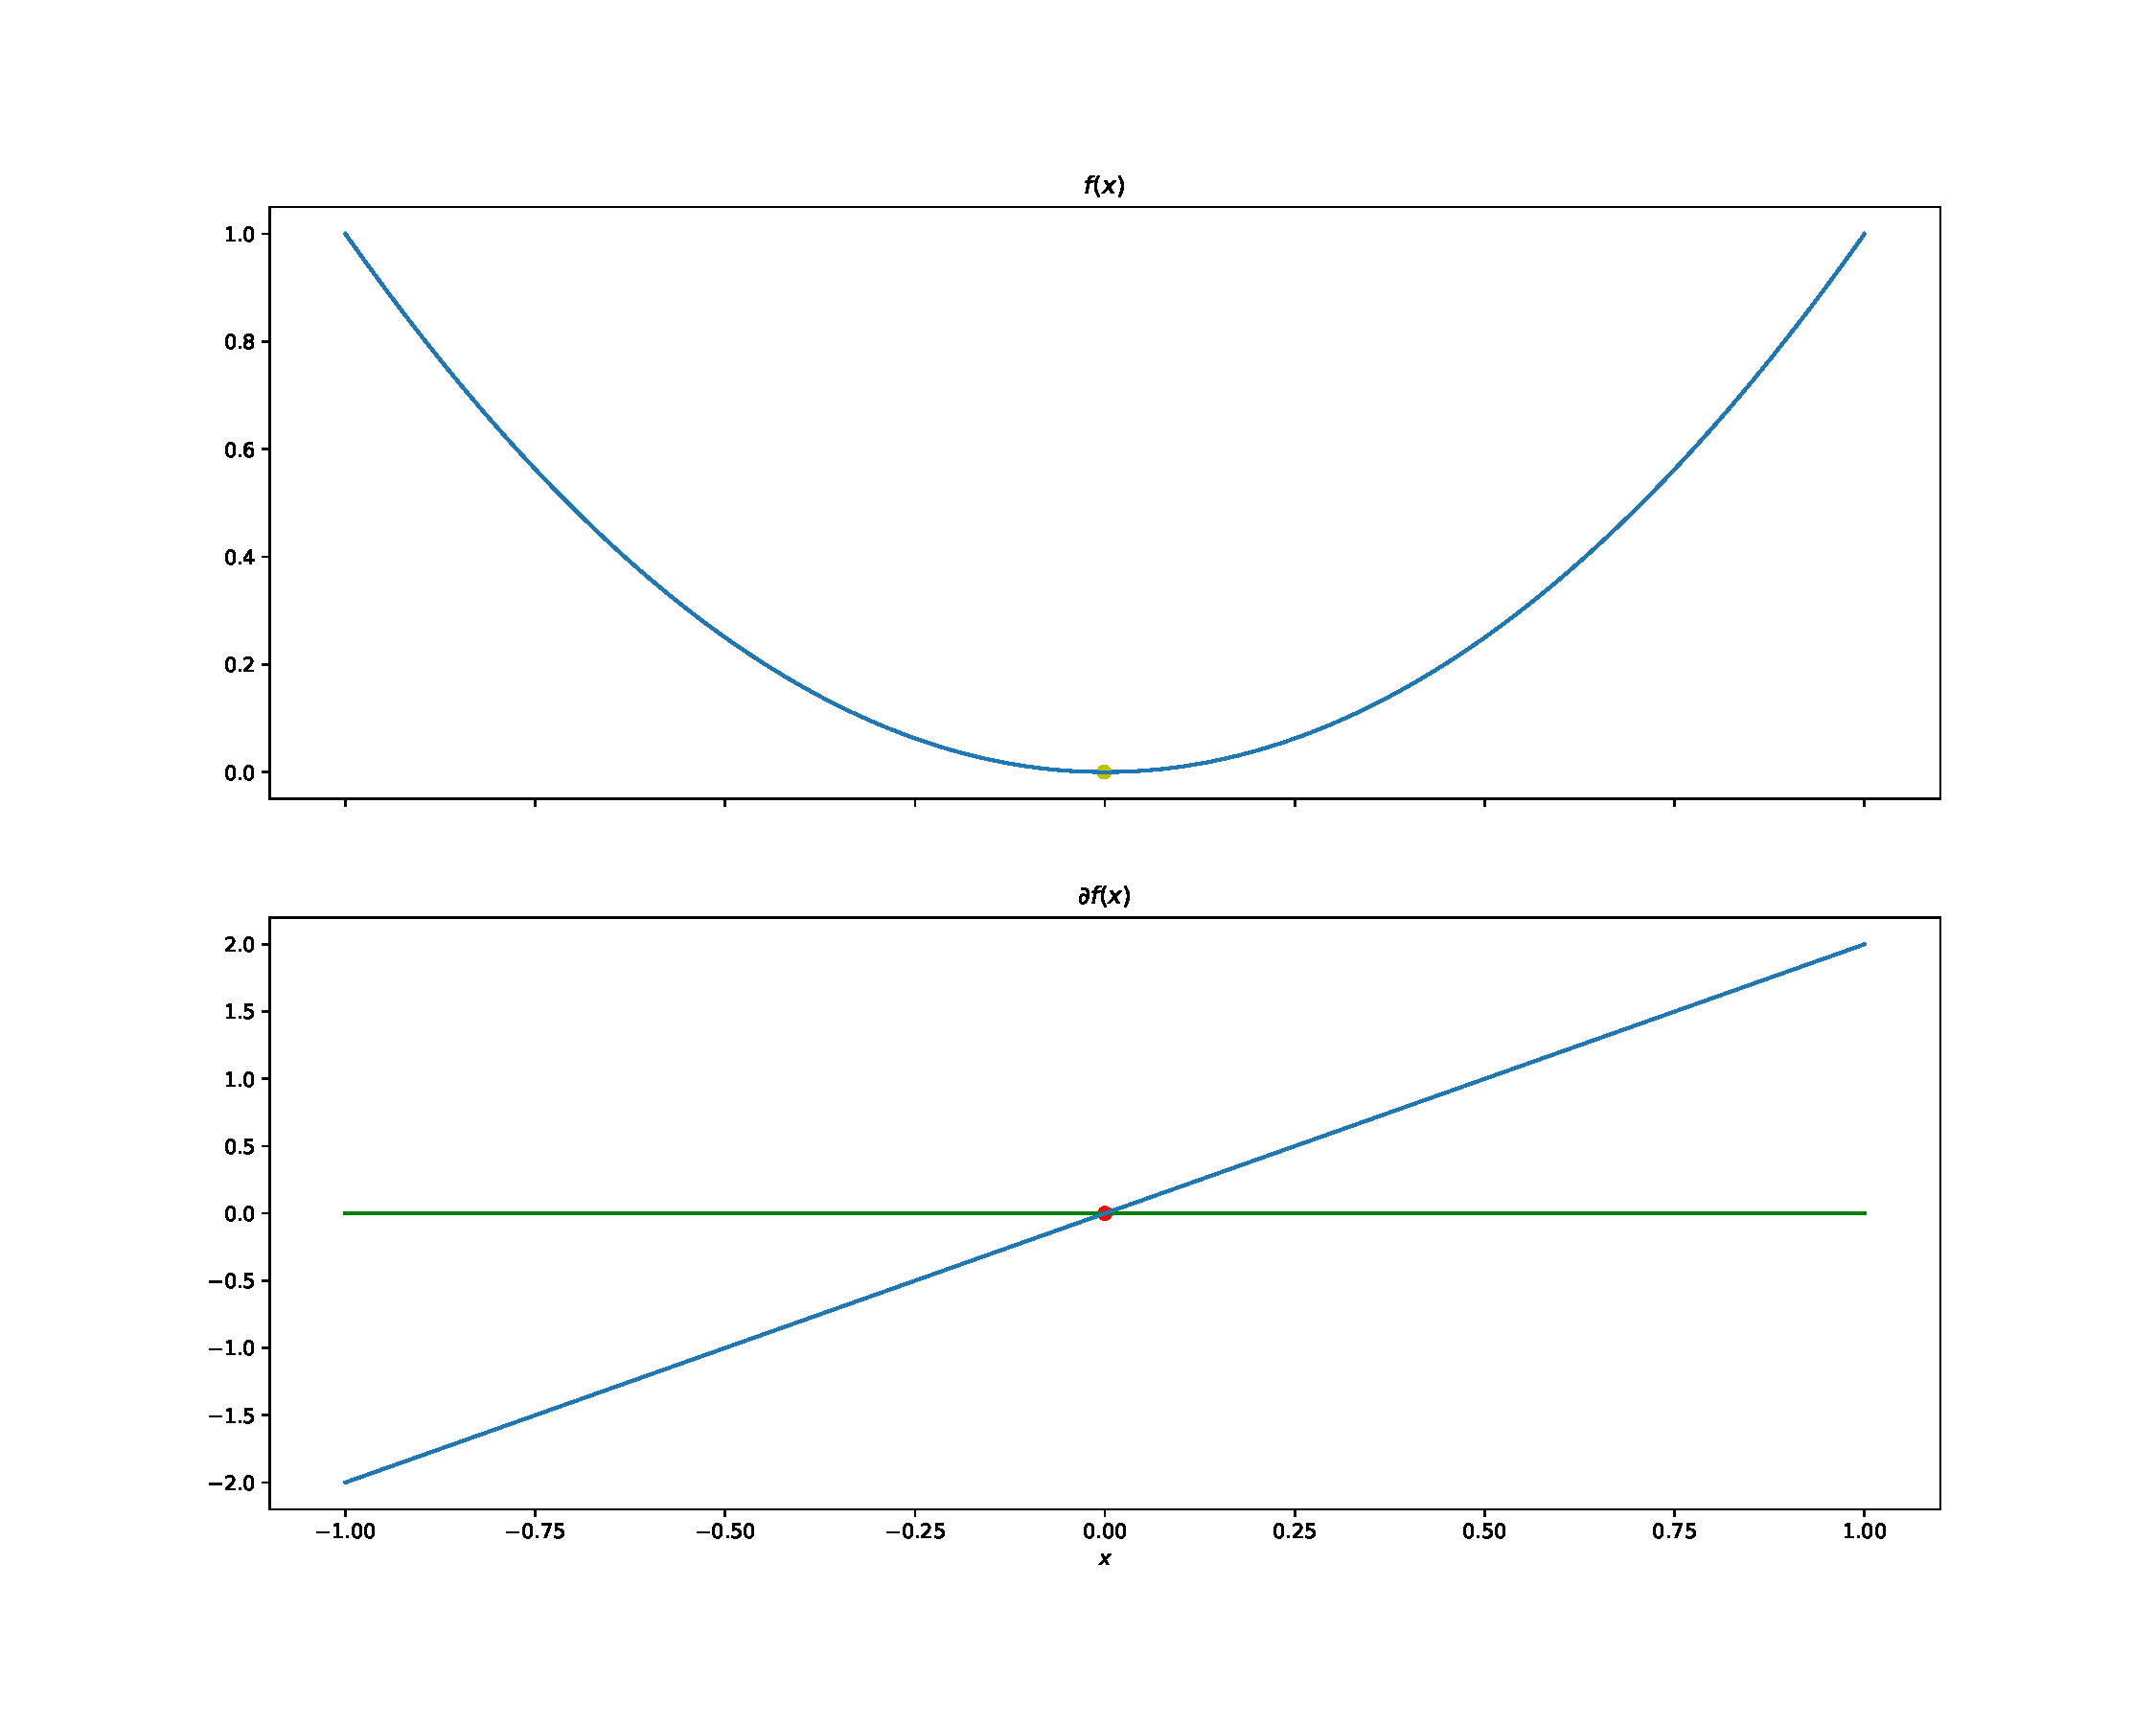
\includegraphics[width=\textwidth]{Chapter4/NeuroCom2021/ejemplo1_mse.pdf}
    \caption{Squared value function (top) and its corresponding subgradient (bottom). The green line represents the $0$ constant function. The yellow dot indicates the point minimizing the function.}
    \label{fig:sq_loss}
\end{figure}
This is the simplest case, since the squared function,
$f(x) = x^2 ,$
is differentiable, and its derivative is 
$\nabla f(x) = 2x$; both are shown in Figure~\ref{fig:sq_loss}.
Using the formulation of~\eqref{eq:subproblem_lambda}, the training error corresponding to the squared loss is
\begin{equation}
    \label{eq:opt_sq}
    \argmin_{\lambda \in [0, 1]} \mathcal{J}(\lambda) = \sum_{i=1}^{\npertask} \left({\lambda c_i + d_i}\right)^2 .
\end{equation}
In this case, $\mathcal{J}(\lambda)$ is a differentiable function, and its gradient is 
\begin{equation}
    \nonumber
    \mathcal{J}'(\lambda) = \sum_{i=1}^\npertask 2 c_i (\lambda c_i + d_i) .
\end{equation}
Solving $\mathcal{J}'(\lambda)= 0$ results in
%
\begin{equation*}
\lambda' =  -\frac{\sum_{i=1}^{\npertask} d_i c_i }{\sum_{i=1}^{\npertask} (c_i)^2 } ,
\end{equation*}
and the optimum is hence $\lambda^* = \max(0, \min(1, \lambda'))$.
\begin{figure}[t!]
    \centering
    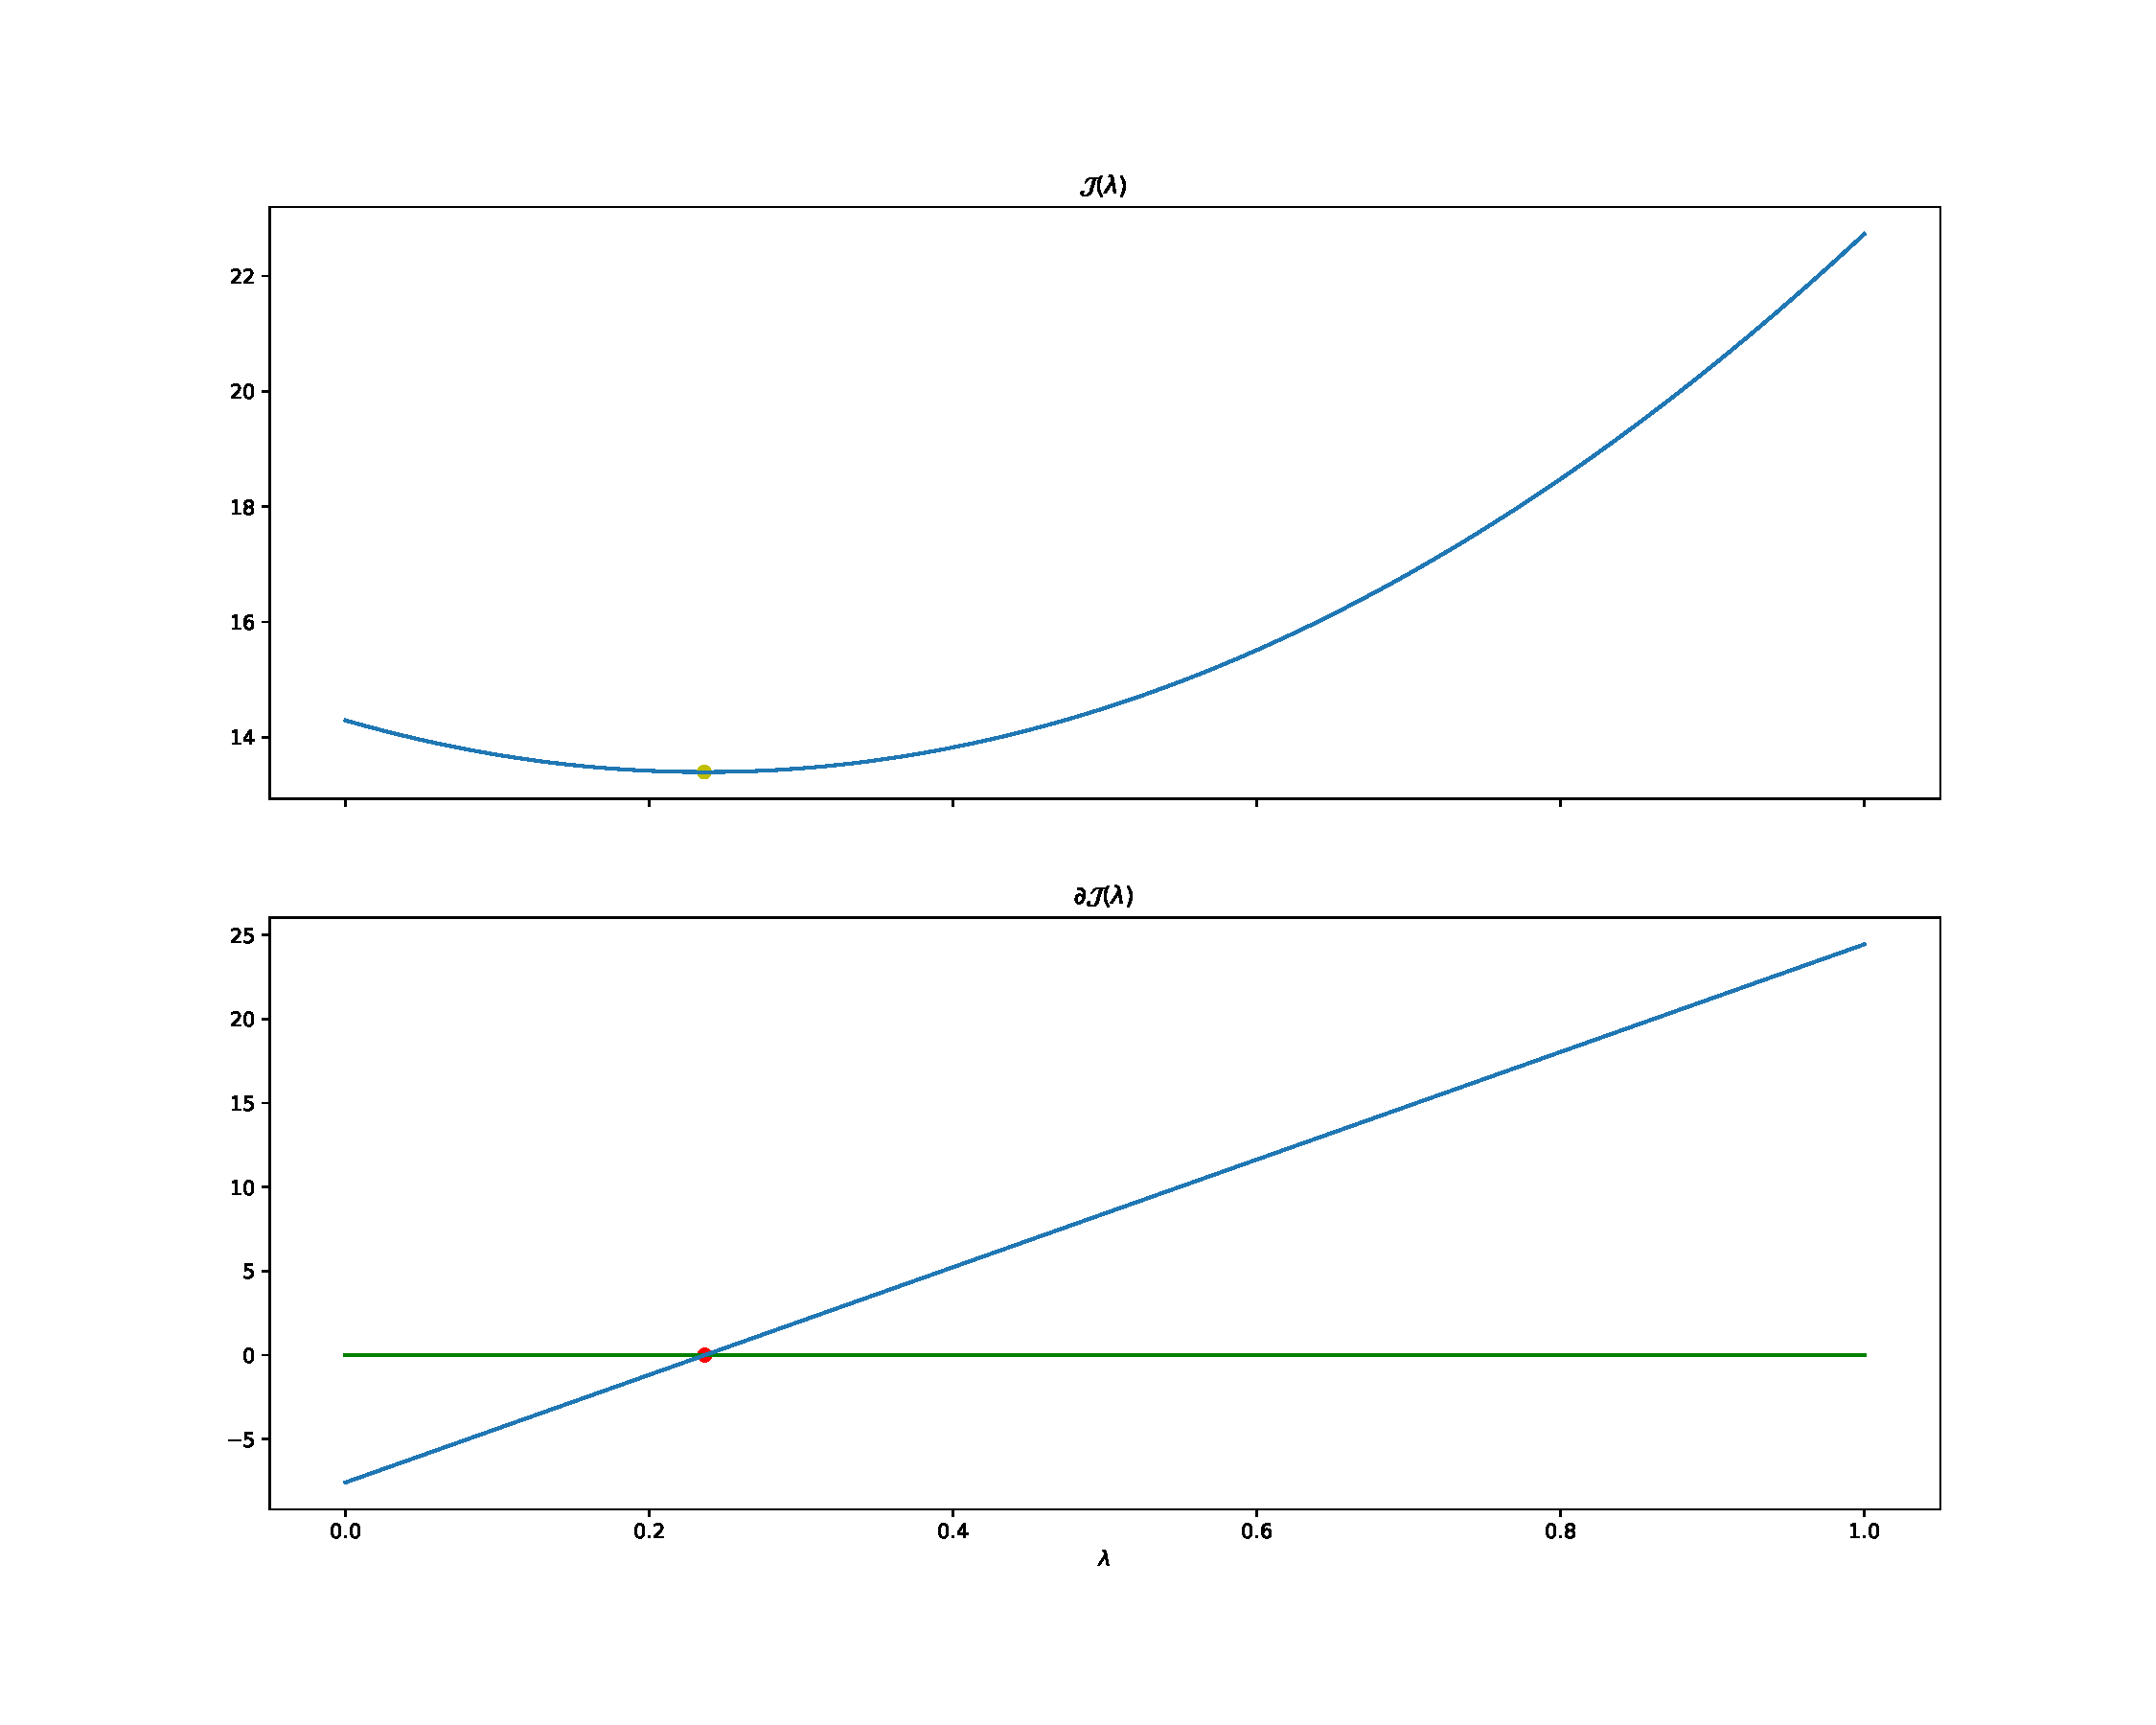
\includegraphics[width=\textwidth]{Chapter4/NeuroCom2021/ejemplo2_mse.pdf}
    \caption{Error using squared loss function (top) and its corresponding subgradient (bottom). The green line represents the $0$ constant function. The yellow dot is the point minimizing the error, and whose corresponding subgradient contains the value $0$.}
    \label{fig:sq_error}
\end{figure}

In Figure~\ref{fig:sq_error} the error function using $10$ random pairs $(c_i, d_i)$ and its corresponding differential is shown.

\paragraph*{Absolute loss.\\}
\begin{figure}[t!]
    \centering
    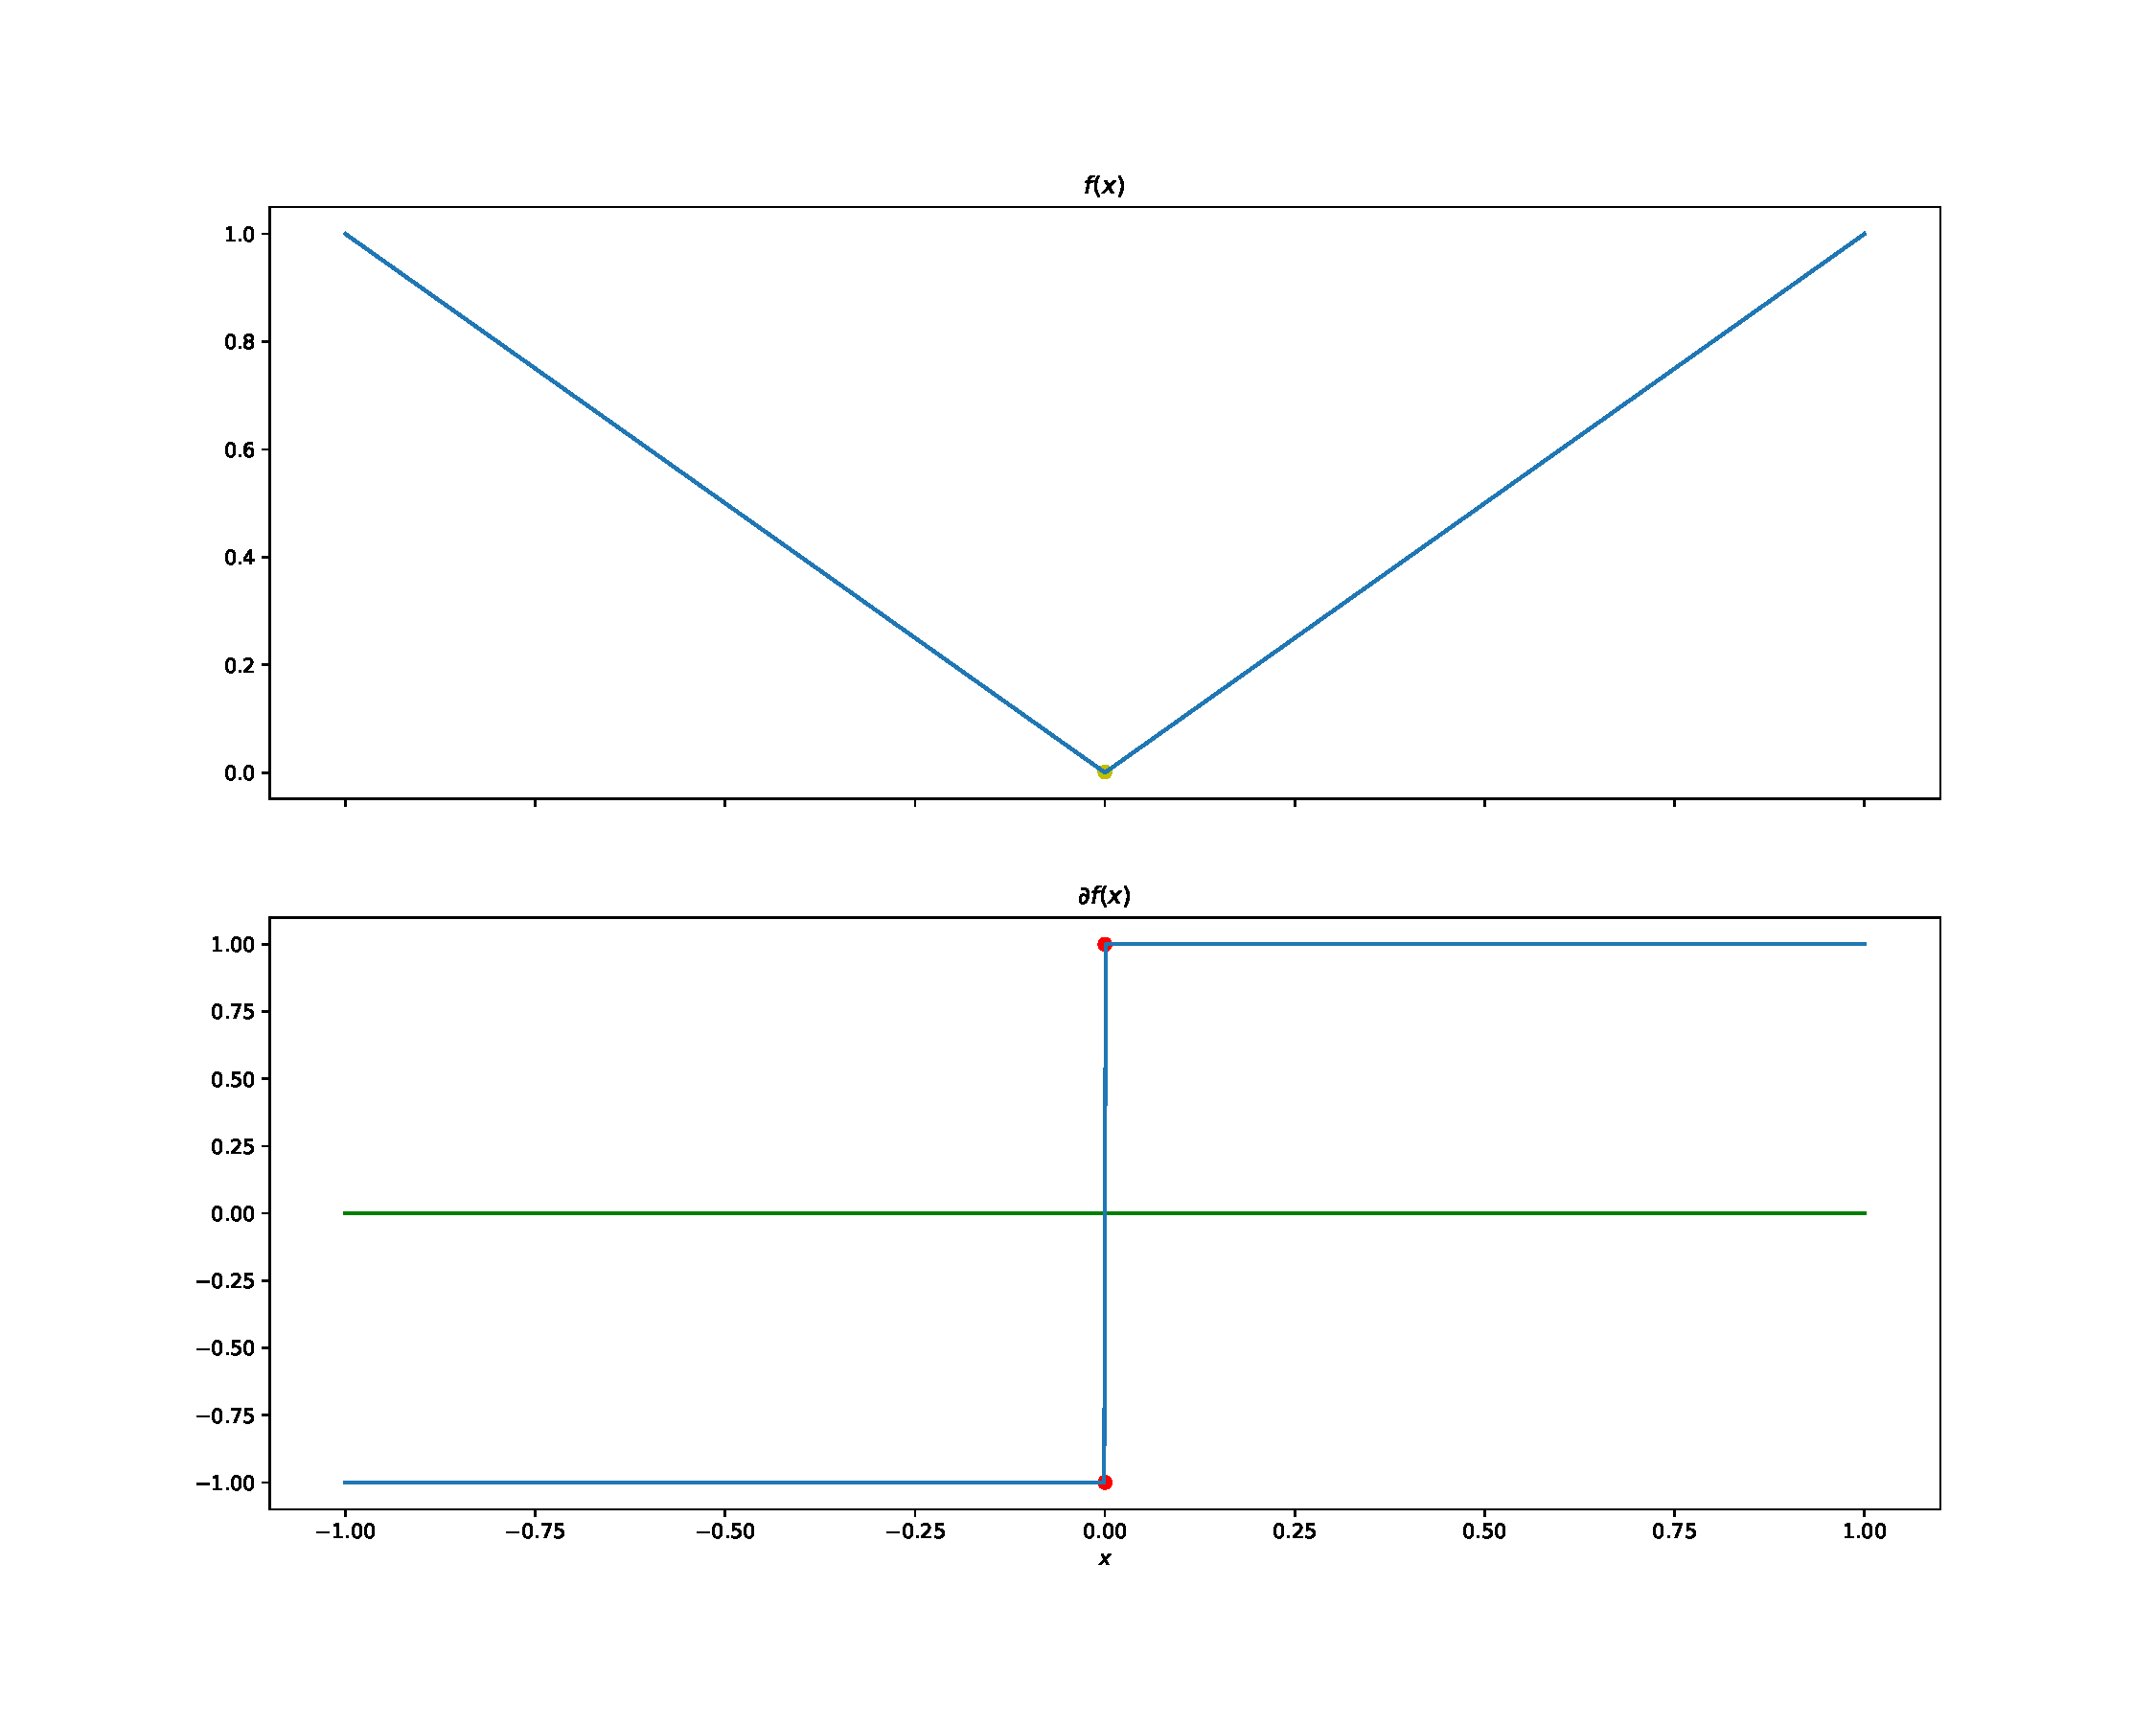
\includegraphics[width=\textwidth]{Chapter4/NeuroCom2021/ejemplo1_mae.pdf}
    \caption{Absolute value function (top) and its corresponding subgradient (bottom). The green line represents the $0$ constant function. The yellow dot indicates the point minimizing the function.}
    \label{fig:abs_loss}
\end{figure}
The absolute function 
\begin{equation}
    \nonumber
    f(x) = 
    \begin{cases}
    -x & x \leq 0, \\
    x & x > 0    
    \end{cases}
\end{equation}
is not differentiable at $0$, but the subgradient can be expressed at any point as
\begin{equation}
    \nonumber
    f(x) = 
    \begin{cases}
    -1 & x < 0, \\
    [-1, 1] & x = 0 , \\
    1 & x > 0 
    \end{cases},
\end{equation}
which is illustrated in Figure~\ref{fig:abs_loss}.
Using the formulation of~\eqref{eq:subproblem_lambda}, the training error corresponding to the absolute value loss is
\begin{equation}
    \label{eq:opt_abs}
    \argmin_{\lambda \in [0, 1]} \mathcal{J}(\lambda) = \sum_{i=1}^{\npertask} \abs{\lambda c_i + d_i}.
\end{equation}
Observe that in each term of the sum the subdifferential is 
\begin{align*}
    \partial \abs{\lambda c_i + d_i} = 
    \begin{cases}
        -\abs{c_i} &, \lambda c_i + d_i  < 0 \\
        [-\abs{c_i}, \abs{c_i}] &, \lambda c_i + d_i  = 0 \\
        \abs{c_i} &, \lambda c_i + d_i  > 0 \\
    \end{cases} 
\end{align*}
The elbows are obtained using the values $\frac{-d_i}{c_i}$, that can be clipped and sorted to get ${\lambda}_{(1)} < \ldots < {\lambda}_{(m)}$.
In~\citet[Proposition 2]{RuizAD21} we present a result to get the optimal $\lambda^*$.
\begin{prop}[Optimal $\lambda^*$ with absolute value loss]\label{prop:abs_neurocom2020}
    In problem~\eqref{eq:opt_abs} $\lambda^*=0$ is optimal iff
    \begin{equation}\nonumber
        - \sum_{j: \lambda_{(j)} < 0} \abs{c_{j}} + \sum_{j: \lambda_{(j)} > 0} \abs{c_{j}} < 0.
        \end{equation}
    If this condition does not hold, $\lambda^* \in (0,1)$ is optimal iff $\lambda^*$ is a feasible elbow, that is, $0 \leq \lambda^* = \lambda_{(k)} \leq 1$ for some $k=1, \dotsc, \npertask$, and
    \begin{equation}\label{sol_abs_e}
    - \sum_{j: \lambda_{(j)} < \lambda_{(k)}} \abs{c_{j}} + \sum_{j: \lambda_{(j)} > \lambda_{(k)}} \abs{c_{j}} \in \left[ -  \abs{c_{k}},  \abs{c_{k}}  \right] .
    \end{equation}
    If none of the previous conditions hold, then $\lambda^*=1$ is optimal.
\end{prop}
\begin{figure}[t!]
    \centering
    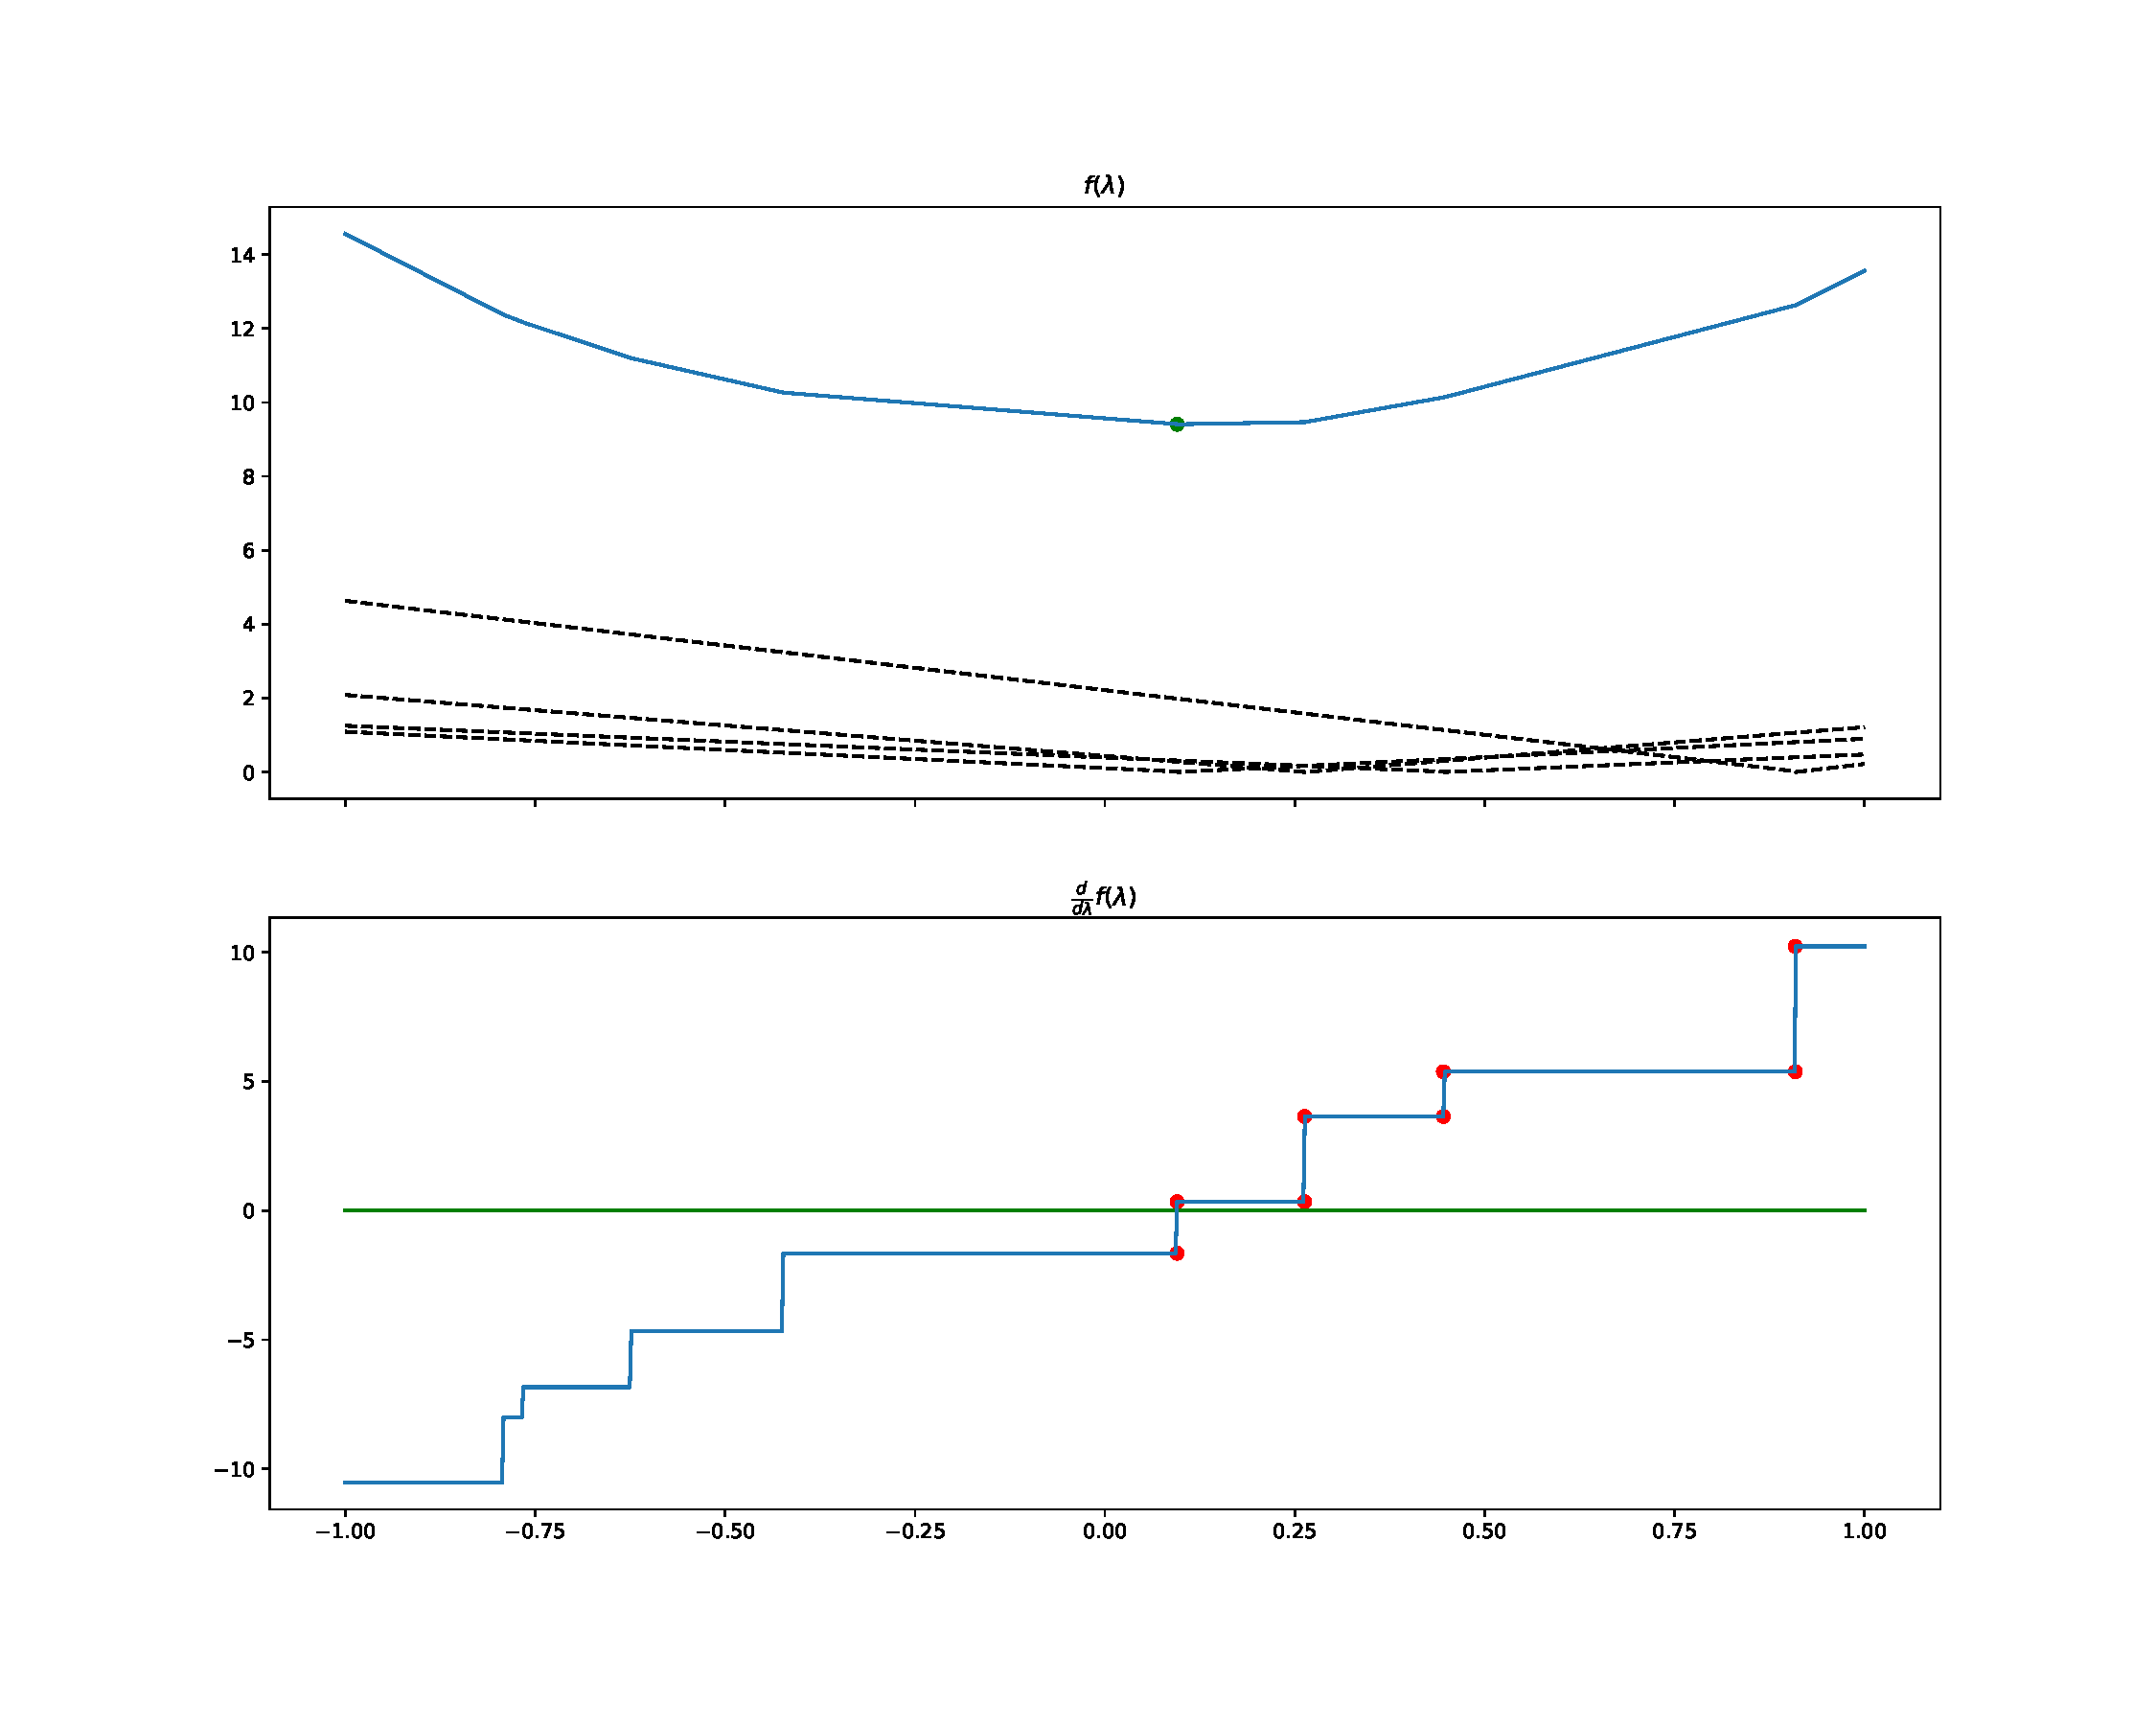
\includegraphics[width=\textwidth]{Chapter4/NeuroCom2021/ejemplo2_mae.pdf}
    \caption{Error using absolute loss function (top) and its corresponding subgradient (bottom). The green line represents the $0$ constant function. Red dots mark the extremes of the subdifferential intervals of non-differentiable points. The yellow dot is the point minimizing the error, and whose corresponding subgradient contains the value $0$.}
    \label{fig:abs_error}
\end{figure}
The result of this proposition is depicted in Figure~\ref{fig:abs_error}, where the error and its corresponding subgradient is computed for $10$ random pairs $(c_i, d_i)$.

\paragraph*{Hinge loss.\\}
The positive part function 
\begin{equation}
    \nonumber
    f(x) = 
    \begin{cases}
    0 & x \leq 0, \\
    x & x > 0    
    \end{cases}
\end{equation}
is not differentiable at $0$, but, again, the subgradient can be expressed at any point as
\begin{equation}
    \nonumber
    f(x) = 
    \begin{cases}
    0 & x < 0, \\
    [0, 1] & x = 0 , \\
    1 & x > 0 
    \end{cases},
\end{equation}
which is illustrated in Figure~\ref{fig:hinge_loss}.
\begin{figure}[t!]
    \centering
    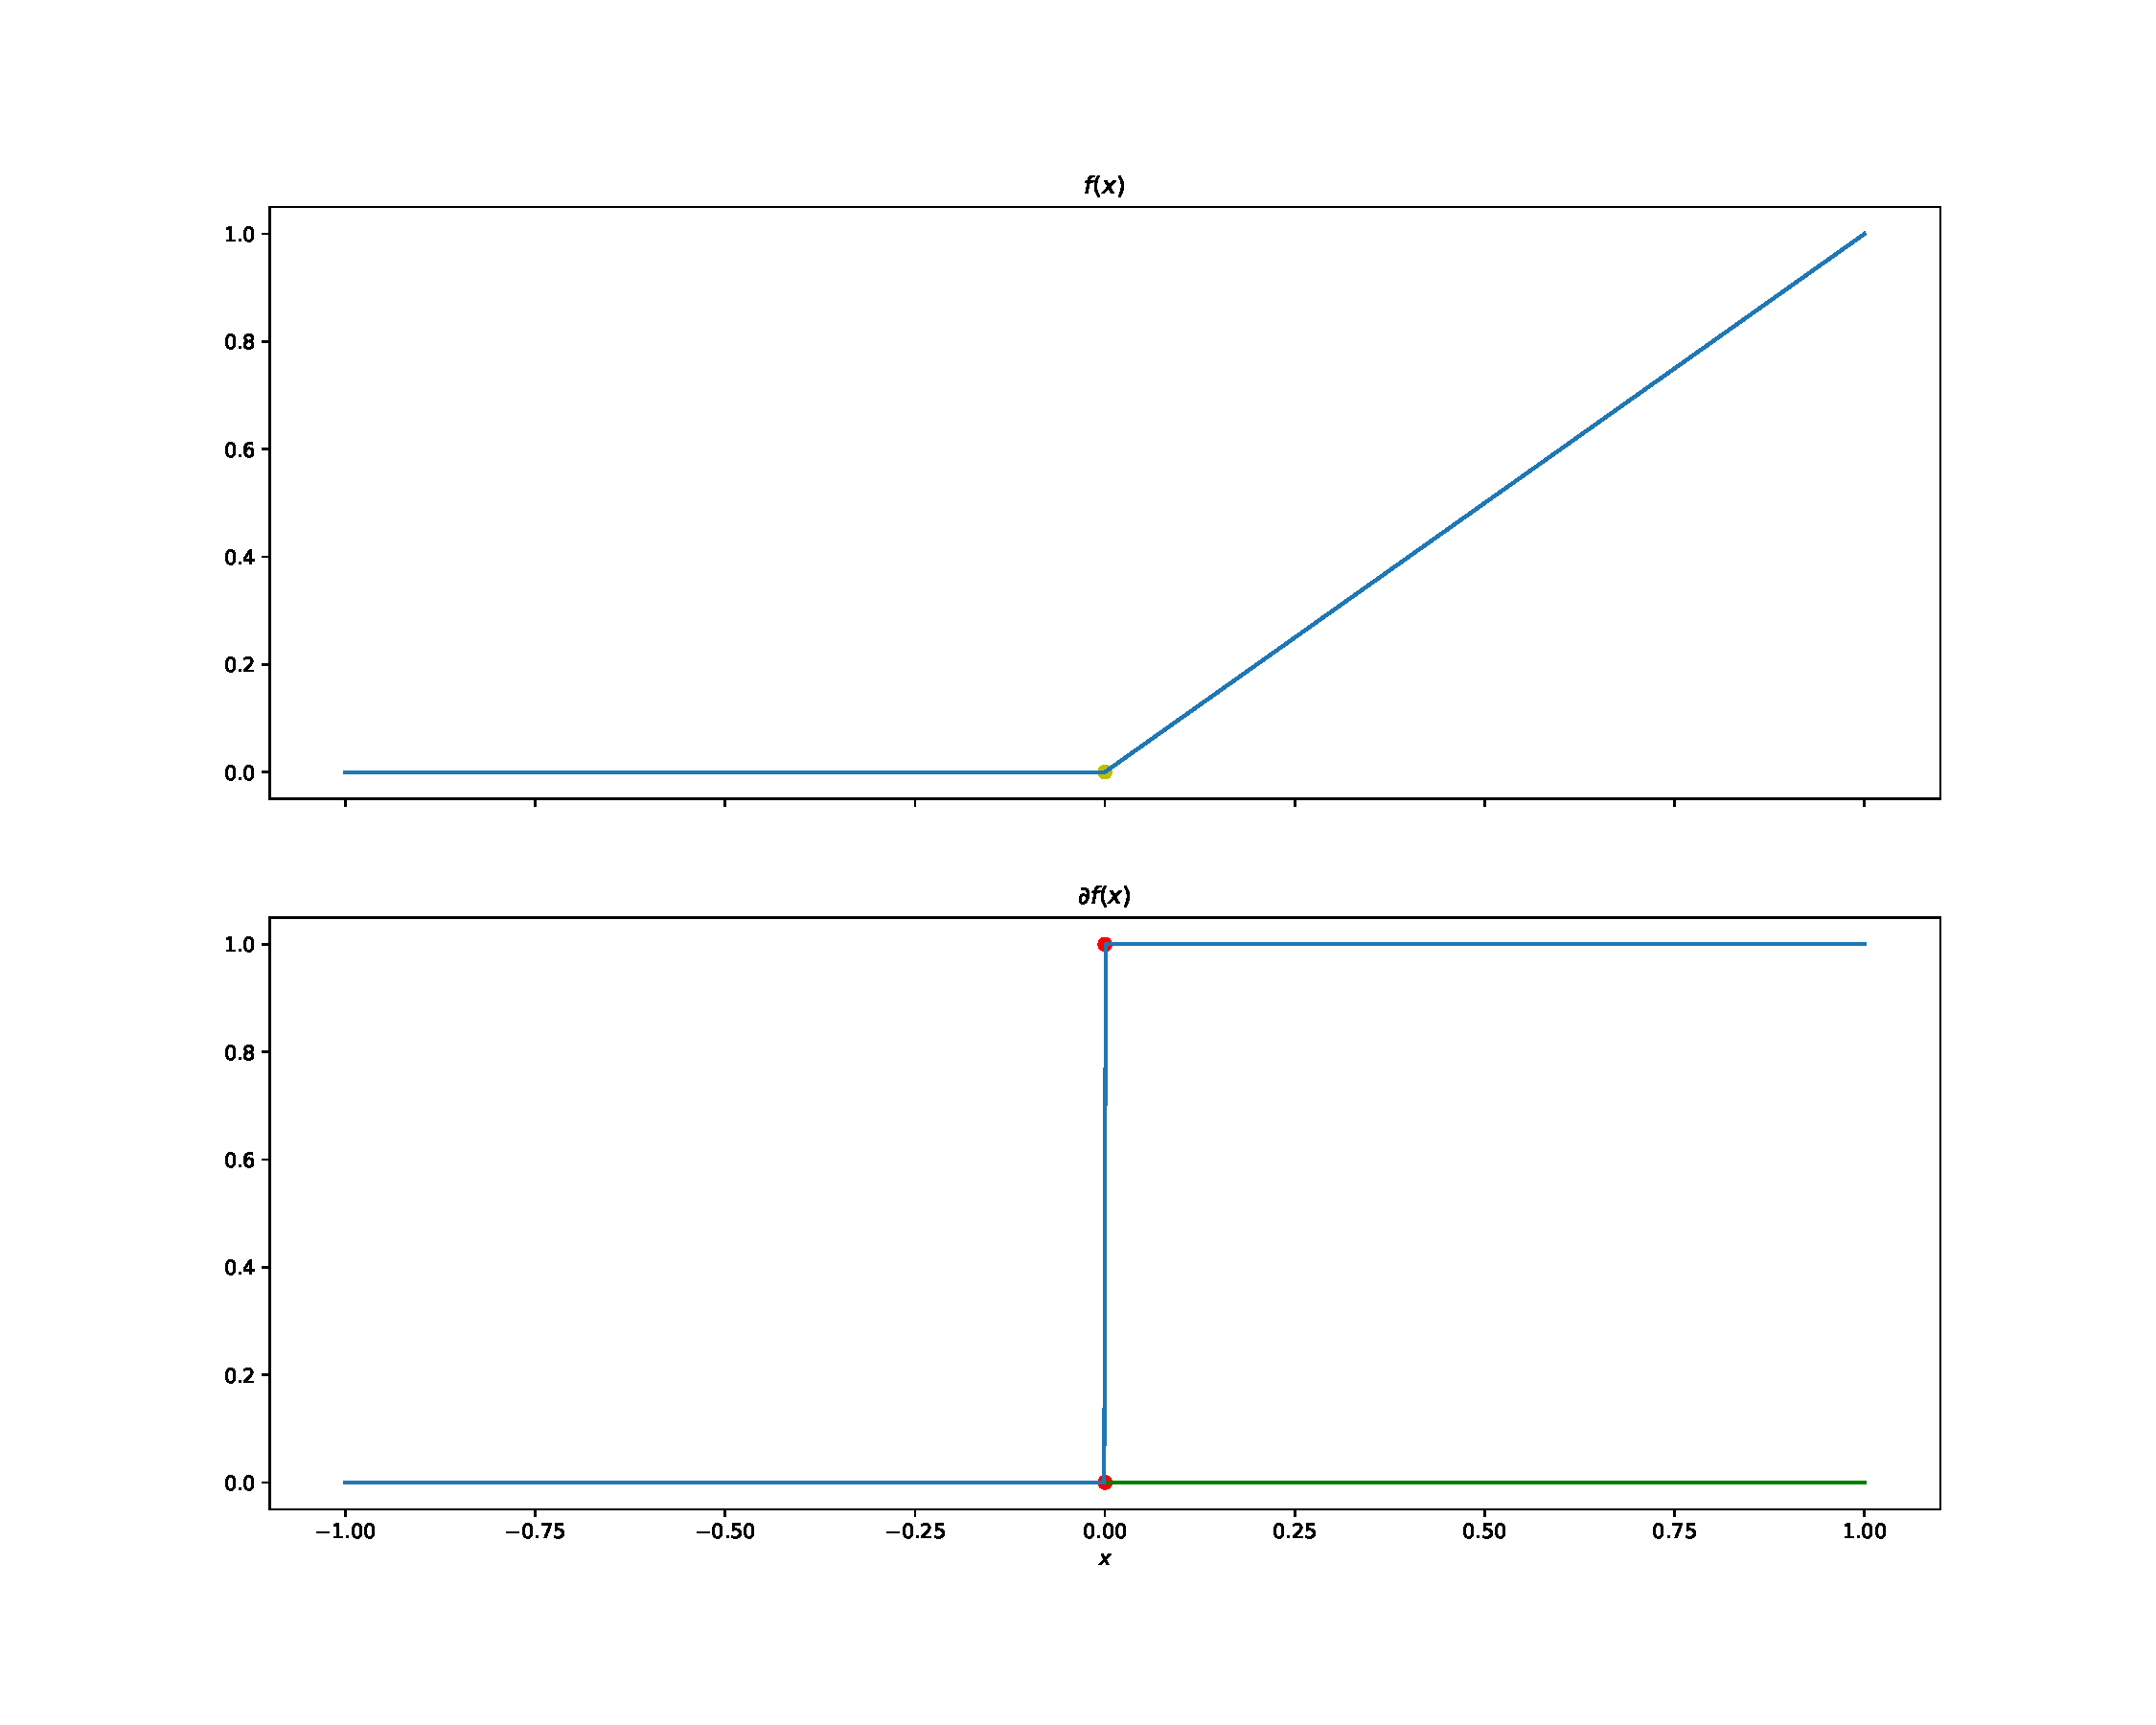
\includegraphics[width=\textwidth]{Chapter4/NeuroCom2021/ejemplo1_hinge.pdf}
    \caption{Positive part function (top) and its corresponding subgradient (bottom). The green line represents the $0$ constant function. The yellow dot indicates the point minimizing the function.}
    \label{fig:hinge_loss}
\end{figure}
Using the formulation of~\eqref{eq:subproblem_lambda}, the training error corresponding to the hinge loss is
\begin{equation}
    \label{eq:opt_hinge_l1}
    \argmin_{\lambda \in [0, 1]} \mathcal{J}(\lambda) = \sum_{i=1}^{\npertask} \pospart{\lambda c_i + d_i}.
\end{equation}
Observe that in each term of the sum the subdifferential is 
\begin{align*}
    \partial \left[\lambda c_i + d_i \right]_+ = 
    \begin{cases}
        0 &, \lambda c_i + d_i  < 0 \\
        [\min(0, c_i), \max(0, c_i)] &, \lambda c_i + d_i  = 0 \\
        c_i &, \lambda c_i + d_i  > 0 \\
    \end{cases} \; .
\end{align*}
That is, the elbows are related to the values $\frac{-d_i}{c_i}$, that can be clipped and sorted to obtain the elbows ${\lambda}_{(1)} < \ldots < {\lambda}_{(m)}$.
In~\citet[Proposition 2]{RuizAD21} we present a result to get the optimal $\lambda^*$.
\begin{prop}[Optimal $\lambda^*$ with hinge loss]\label{prop:hinge_neurocom2020}
    In~\eqref{eq:opt_hinge_l1}, $\lambda^*=0$ is optimal iff
    \begin{equation}\label{eq:sol_hinge_0}
        -\sum_{j: \lambda_{(j)}<0} \max(0, c_{(j)}) - \sum_{\lambda_{(j)}>0} \min(0, c_{(j)}) \leq 0 .
        \end{equation}
        If this condition does not hold, a value $\lambda^* \in (0, 1)$ is optimal for problem~\eqref{eq:opt_hinge_l1} iff $\lambda^* \in \set{0, 1}$ or $\lambda^*$ is a feasible elbow, that is, $0 \leq \lambda^* = \lambda_{(k)} \leq 1$ for some $k=1, \dotsc, \npertask$, and
    \begin{equation}\label{eq:sol_hinge}
        -\sum_{j: \lambda_{(j)}< \lambda_{(k)}} \max(0, c_{(j)}) - \sum_{j: \lambda_{(j)}>  \lambda_{(k)}} \min(0, c_{(j)}) \in \left[\min(0, c_{(k)}), \max(0, c_{(k)}) \right] .
    \end{equation}
    If none of the previous conditions hold, then $\lambda^*=1$ is optimal.
\end{prop}
\begin{figure}[t!]
    \centering
    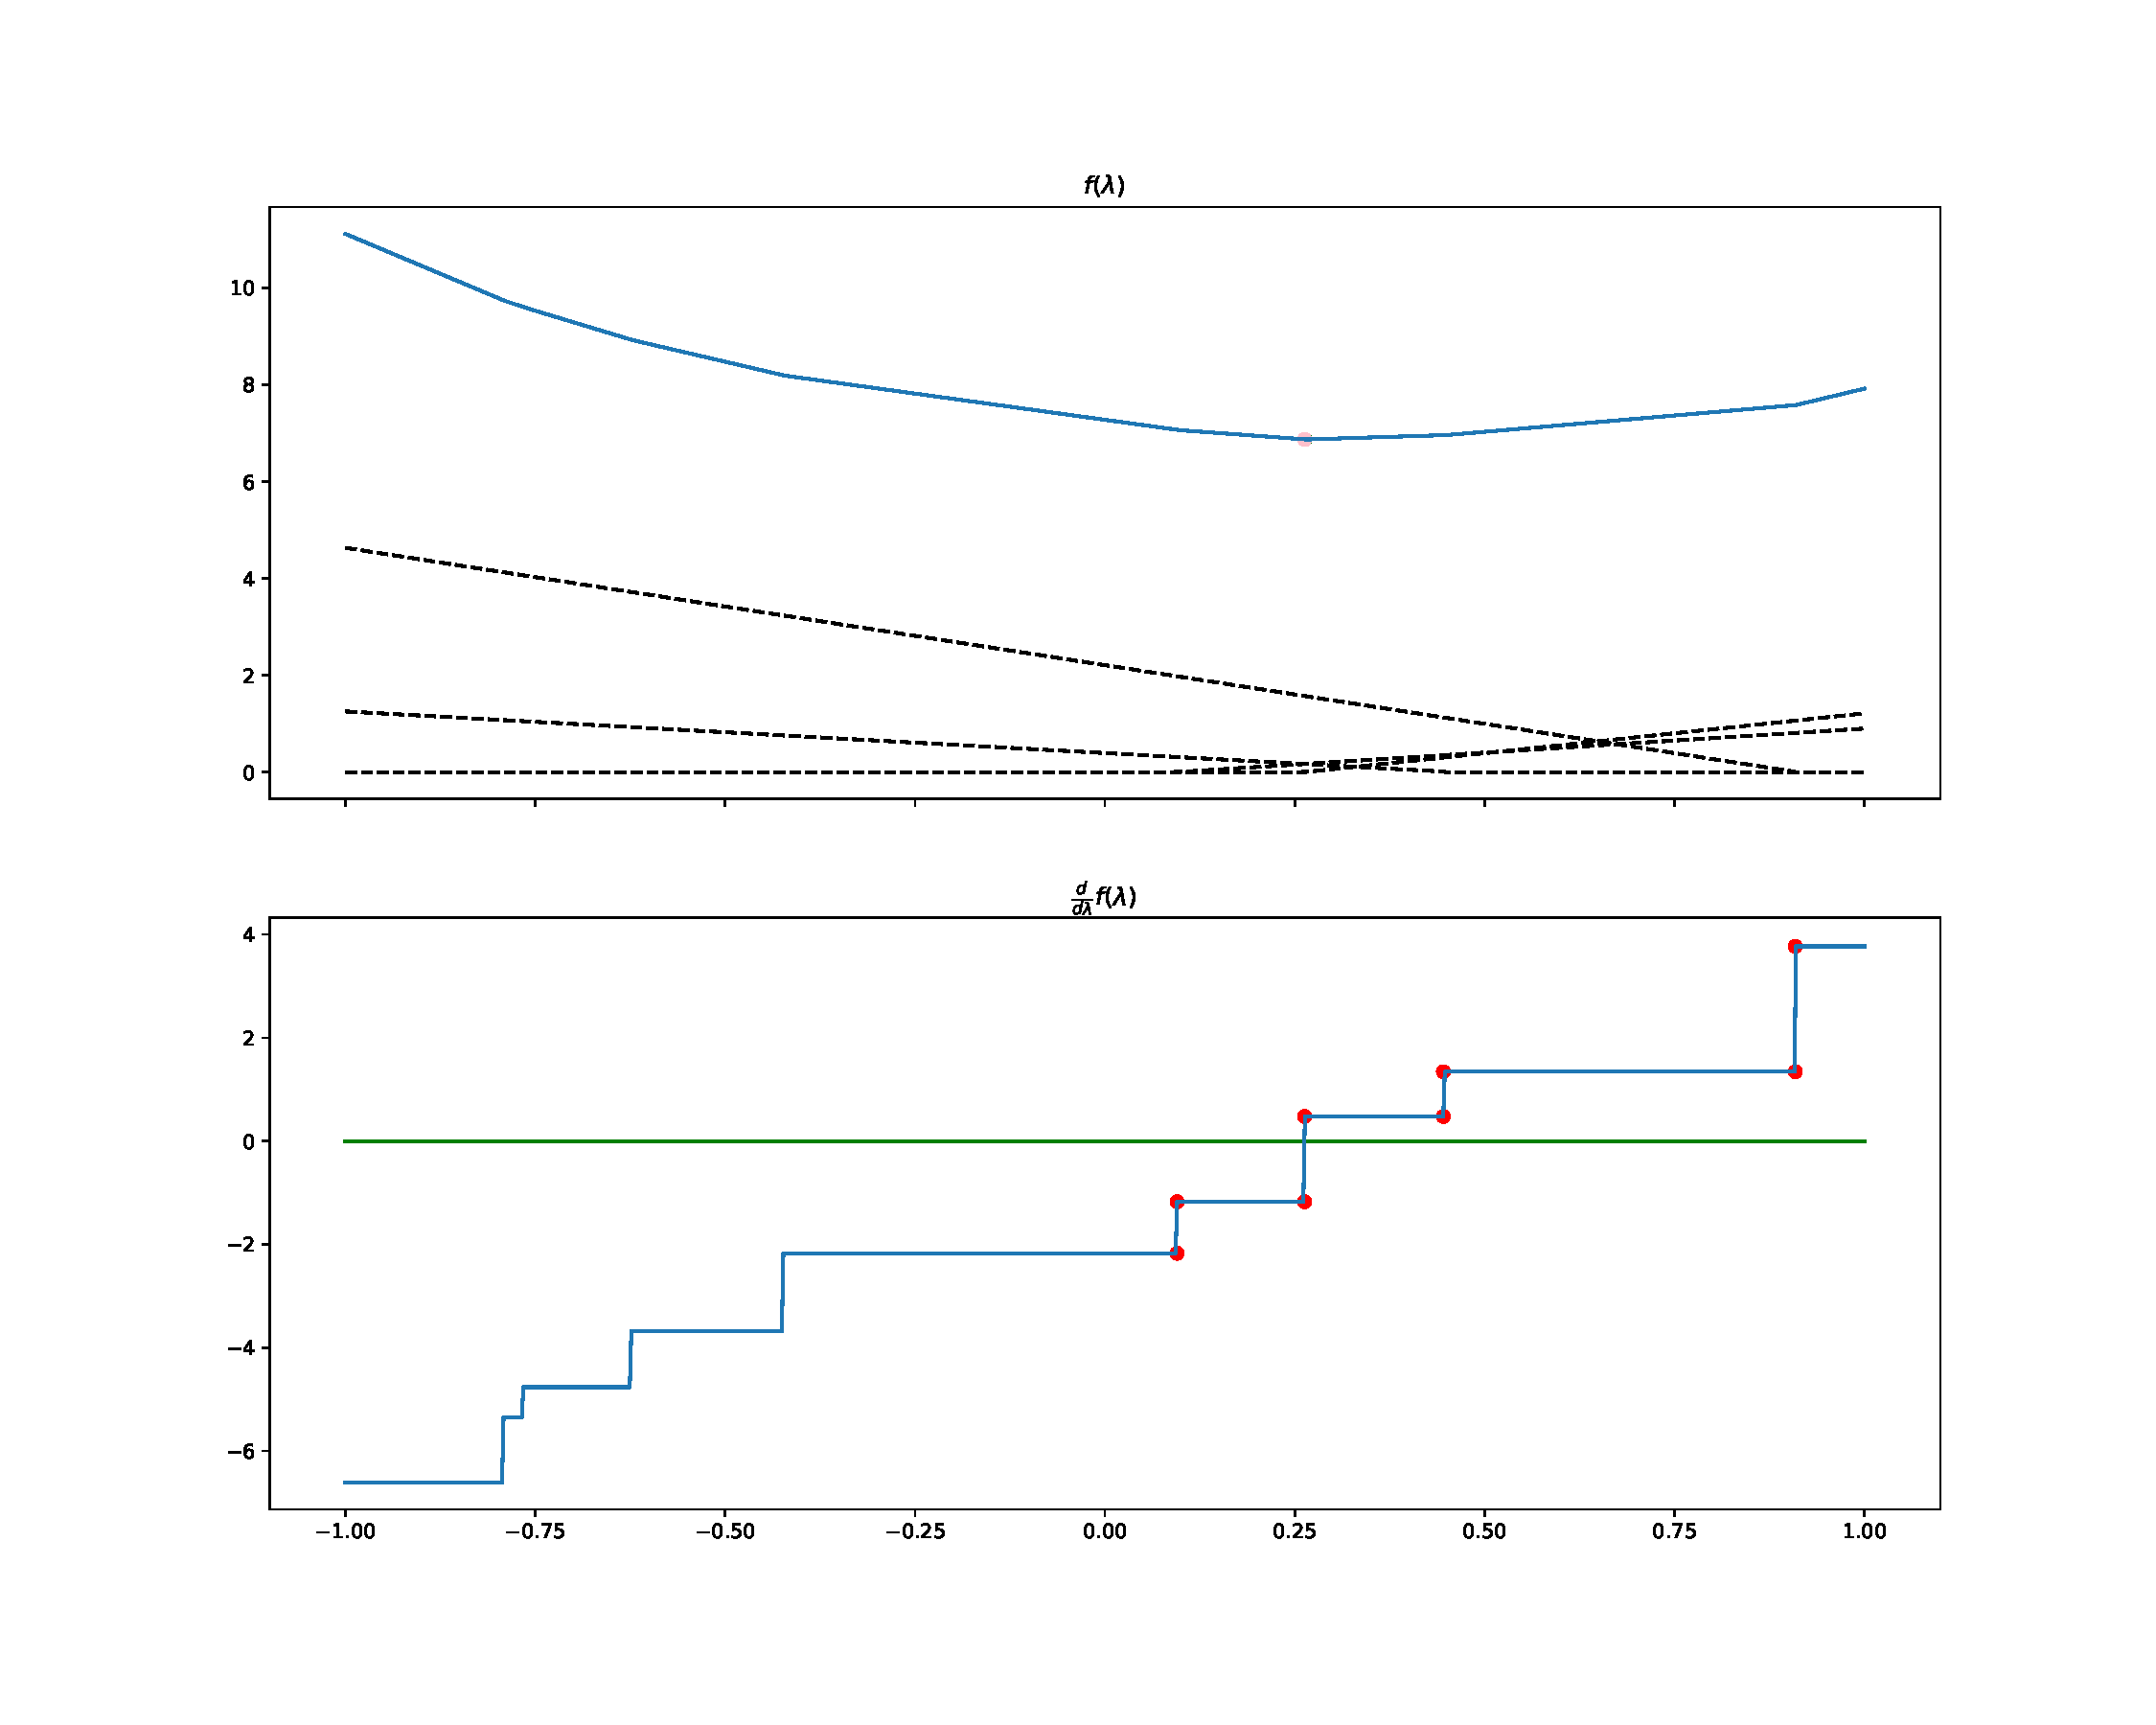
\includegraphics[width=\textwidth]{Chapter4/NeuroCom2021/ejemplo2_hinge.pdf}
    \caption{Error using hinge loss function (top) and its corresponding subgradient (bottom). The green line represents the $0$ constant function. Red dots mark the extremes of the subdifferential intervals of non-differentiable points. The yellow dot is the point minimizing the error, and whose corresponding subgradient contains the value $0$.}
    \label{fig:hinge_error}
\end{figure}

Again, the results of the proposition are illustrated in Figure~\ref{fig:hinge_error}, where $10$ pairs $(c_i, d_i)$ are randomly sampled, and the corresponding error function $\mathcal{J}(\lambda)$ and its subgradient are shown.

\paragraph*{Squared hinge loss.\\}
The squared positive part function is
\begin{equation}
    \nonumber
    f(x) = 
    \begin{cases}
    0 & x \leq 0, \\
    x^2 & x > 0    
    \end{cases}
\end{equation}
and its gradient can be expressed at any point as
\begin{equation}
    \nonumber
    f(x) = 
    \begin{cases}
    0 & x \leq 0, \\
    2x & x > 0 
    \end{cases},
\end{equation}
which is illustrated in Figure~\ref{fig:hinge_loss}.
Although the gradient can be defined at any point, the definition by parts makes it difficult to obtain results.
\begin{figure}[t!]
    \centering
    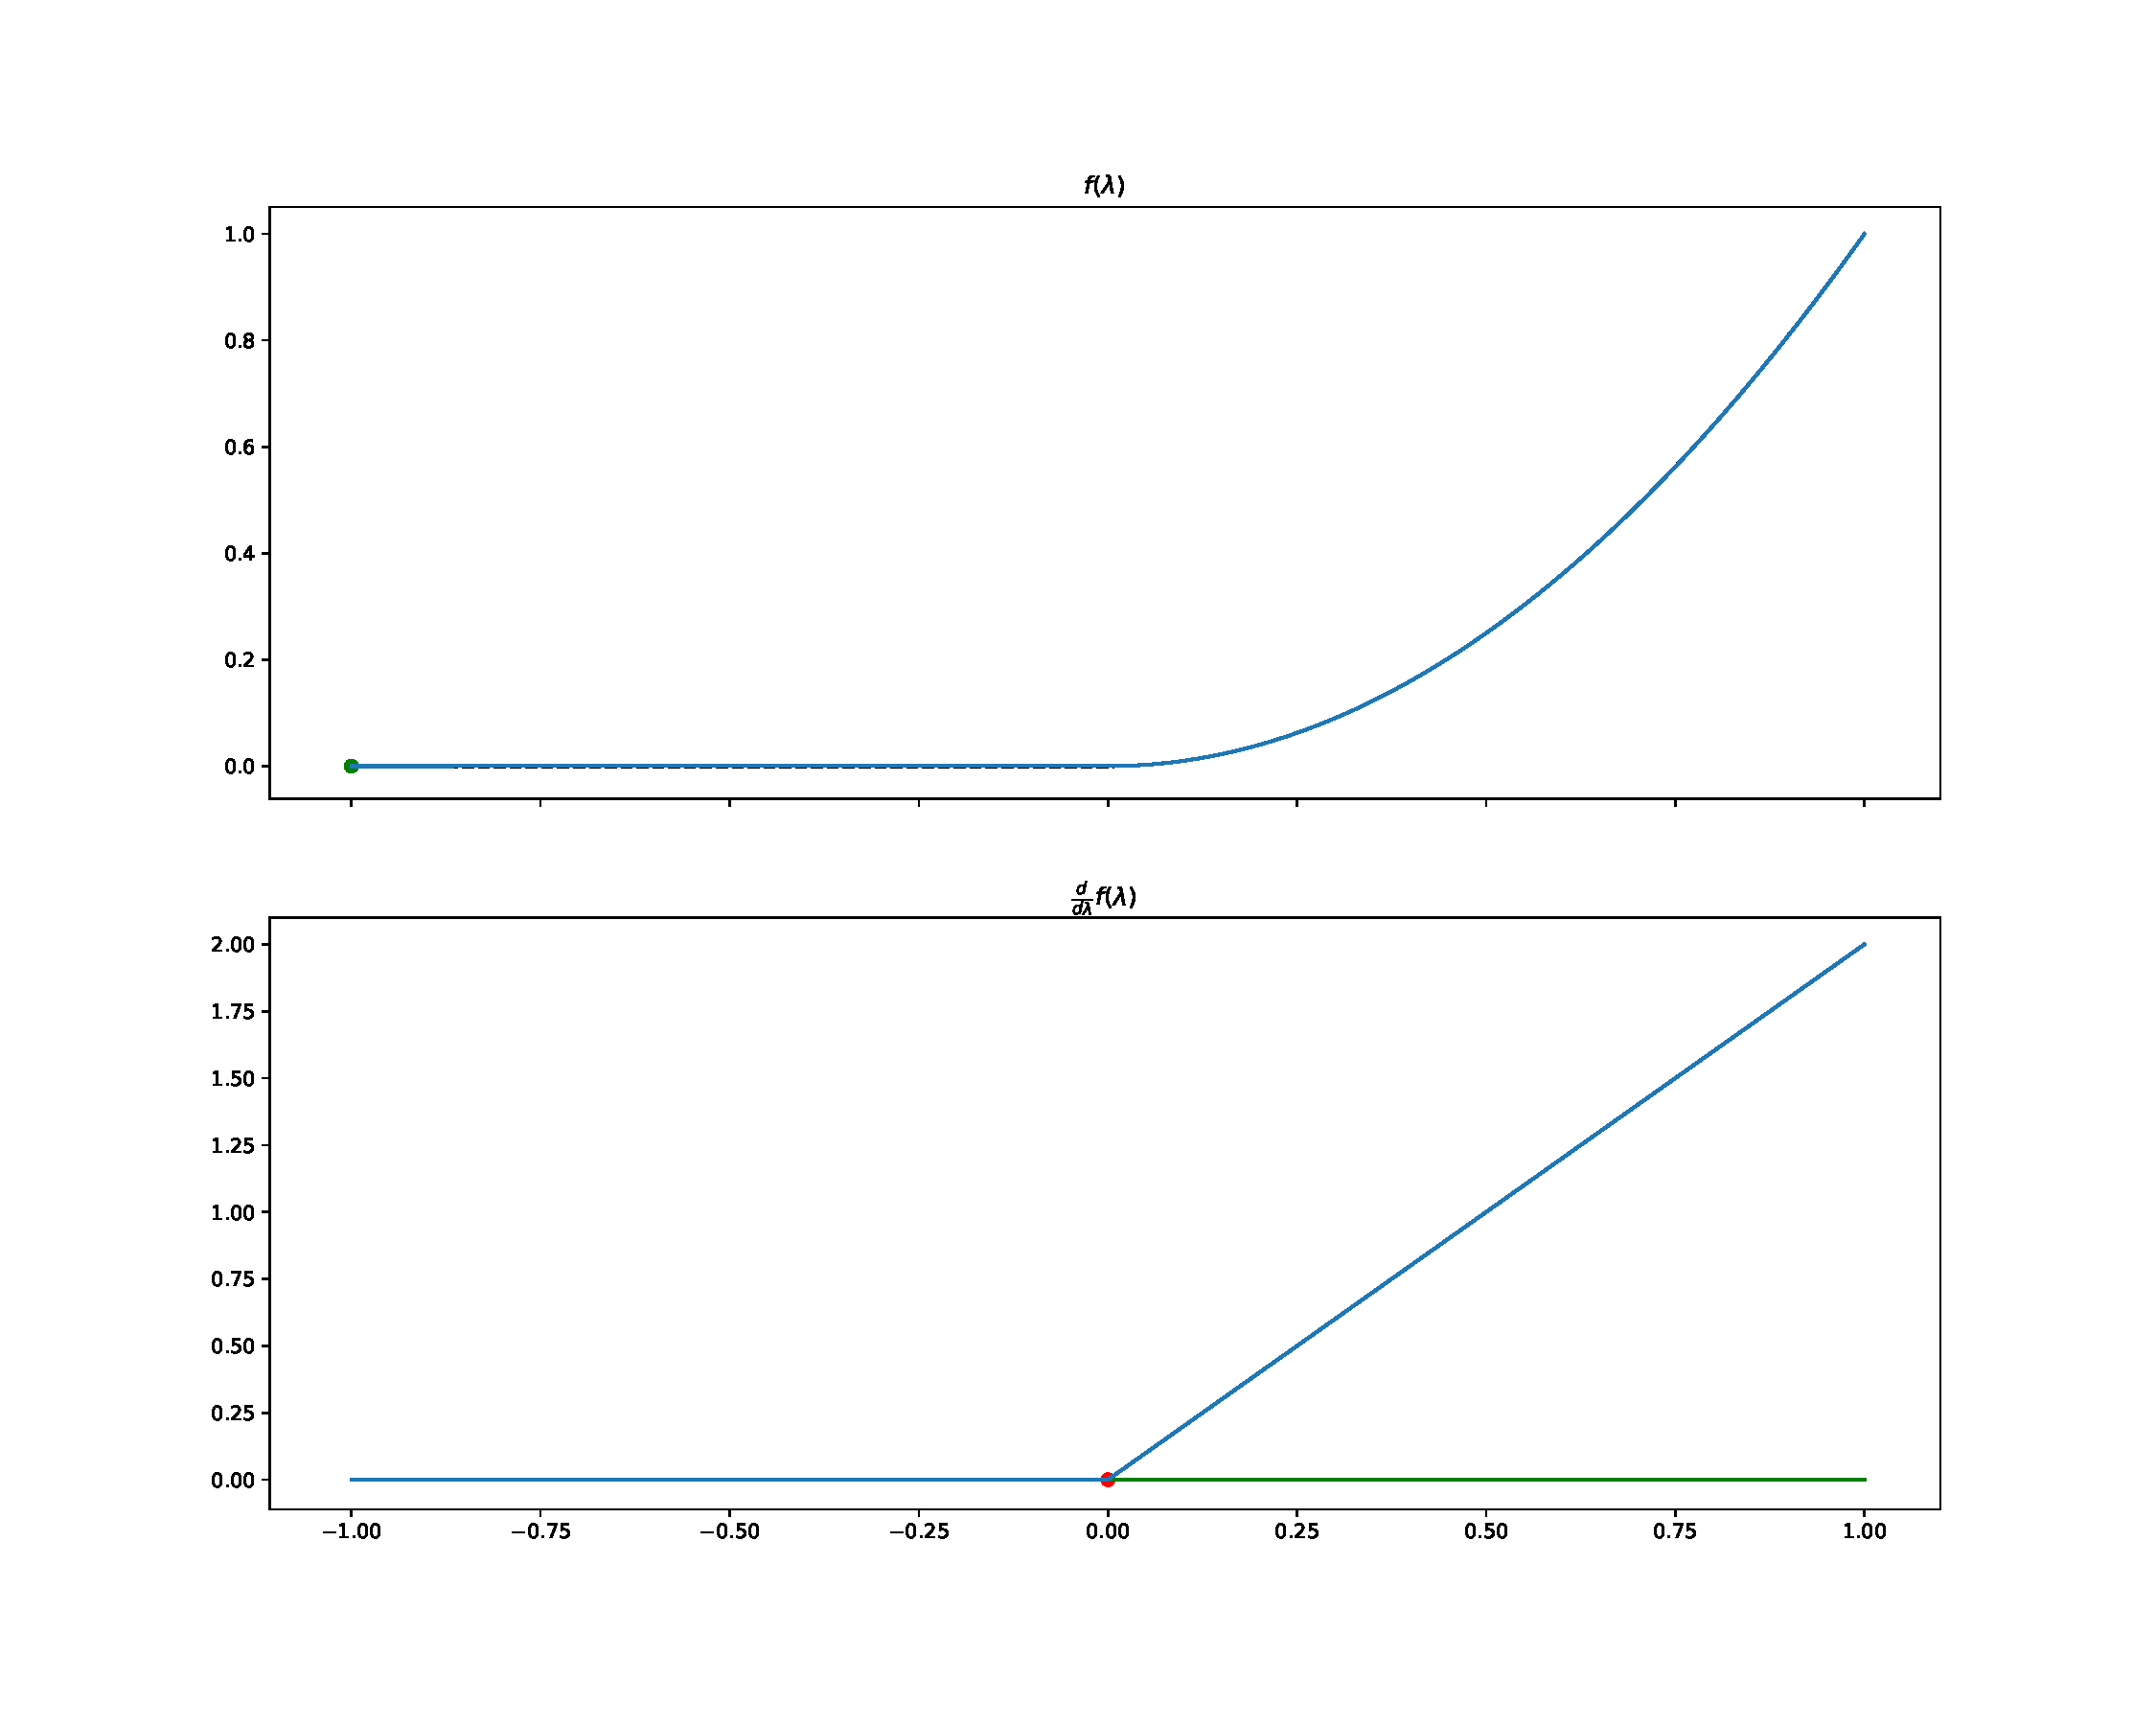
\includegraphics[width=\textwidth]{Chapter4/NeuroCom2021/ejemplo1_sqhinge.pdf}
    \caption{Positive part function (top) and its corresponding subgradient (bottom). The green line represents the $0$ constant function. The yellow dot indicates the point minimizing the function.}
    \label{fig:sqhinge_loss}
\end{figure}
Using the formulation of~\eqref{eq:subproblem_lambda}, the training error corresponding to the hinge loss is
\begin{equation}
    \label{eq:opt_hinge_l2}
    \argmin_{\lambda \in [0, 1]} \mathcal{J}(\lambda) = \sum_{i=1}^{\npertask} \pospart{\lambda c_i + d_i}^2.
\end{equation}
In each term of the sum the subdifferential is 
\begin{align*}
    \partial \left[\lambda c_i + d_i \right]_+^2 = 
    \begin{cases}
        0 &, \lambda c_i + d_i  \leq 0 \\
        2 c_i (\lambda c_i + d_i) &, \lambda c_i + d_i  > 0 \\
    \end{cases} \; .
\end{align*}
The elbows are again related to the values $\frac{-d_i}{c_i}$, that can be clipped and sorted to obtain the elbows ${\lambda}_{(1)} < \ldots < {\lambda}_{(m)}$.
In~\citet[Proposition 2]{RuizAD21} we give a result to get the optimal $\lambda^*$ when using the squared hinge loss.
\begin{prop}[Optimal $\lambda^*$ with squared hinge loss]\label{prop:sqhinge_neurocom2020}
    In~\eqref{eq:opt_hinge_l2},
    $\lambda^*=0$ is optimal iff 
    \begin{equation}\nonumber
         - \frac{\sum_{j: \lambda_{j} < 0} \max(0, c_{j}) d_{j} + \sum_{j: \lambda_{j} > 0} \min(0, c_{j}) d_{j}}{\sum_{j: \lambda_{j} < 0} \max(0, c_{j})^2 + \sum_{j: \lambda_{j} > 0} \min(0, c_{j})^2} < 0.
       \end{equation}
    If this condition does not hold, 
    consider the extended sorted list of feasible elbows $\lambda_{(p-1)} = 0 \leq \lambda_{(p)} \leq \ldots, \lambda_{(q)} \leq \lambda_{(q+1)}=1$, with $1 \leq p, q \leq m$, and
    define for $k=p-1, \ldots,  q$ $\widehat{\lambda}_k$ as %
\begin{equation}\label{sol_hinge_2}
 \widehat{\lambda}_k = - \frac{\sum_{j: \lambda_{(j)} < \lambda_{(k)}} \max(0, c_{j}) d_{j} + \sum_{j: \lambda_{(j)} > \lambda_{(k)}} \min(0, c_{j}) d_{j}}{\sum_{j: \lambda_{(j)} < \lambda_{(k)}} \max(0, c_{j})^2 + \sum_{j: \lambda_{(j)} > \lambda_{(k)}} \min(0, c_{j})^2} .
\end{equation}
%
Then, if $\lambda_k \leq \widehat{\lambda}_k \leq  \lambda_{k+1}$ for some $\widehat{\lambda}_k$, then $\lambda^* = \widehat{\lambda}_k$ is optimal.
Finally, if none of the previous conditions holds, \eqref{eq:opt_hinge_l2} has a minimum at $\lambda^* = 1$.
\end{prop}
\begin{figure}[t!]
    \centering
    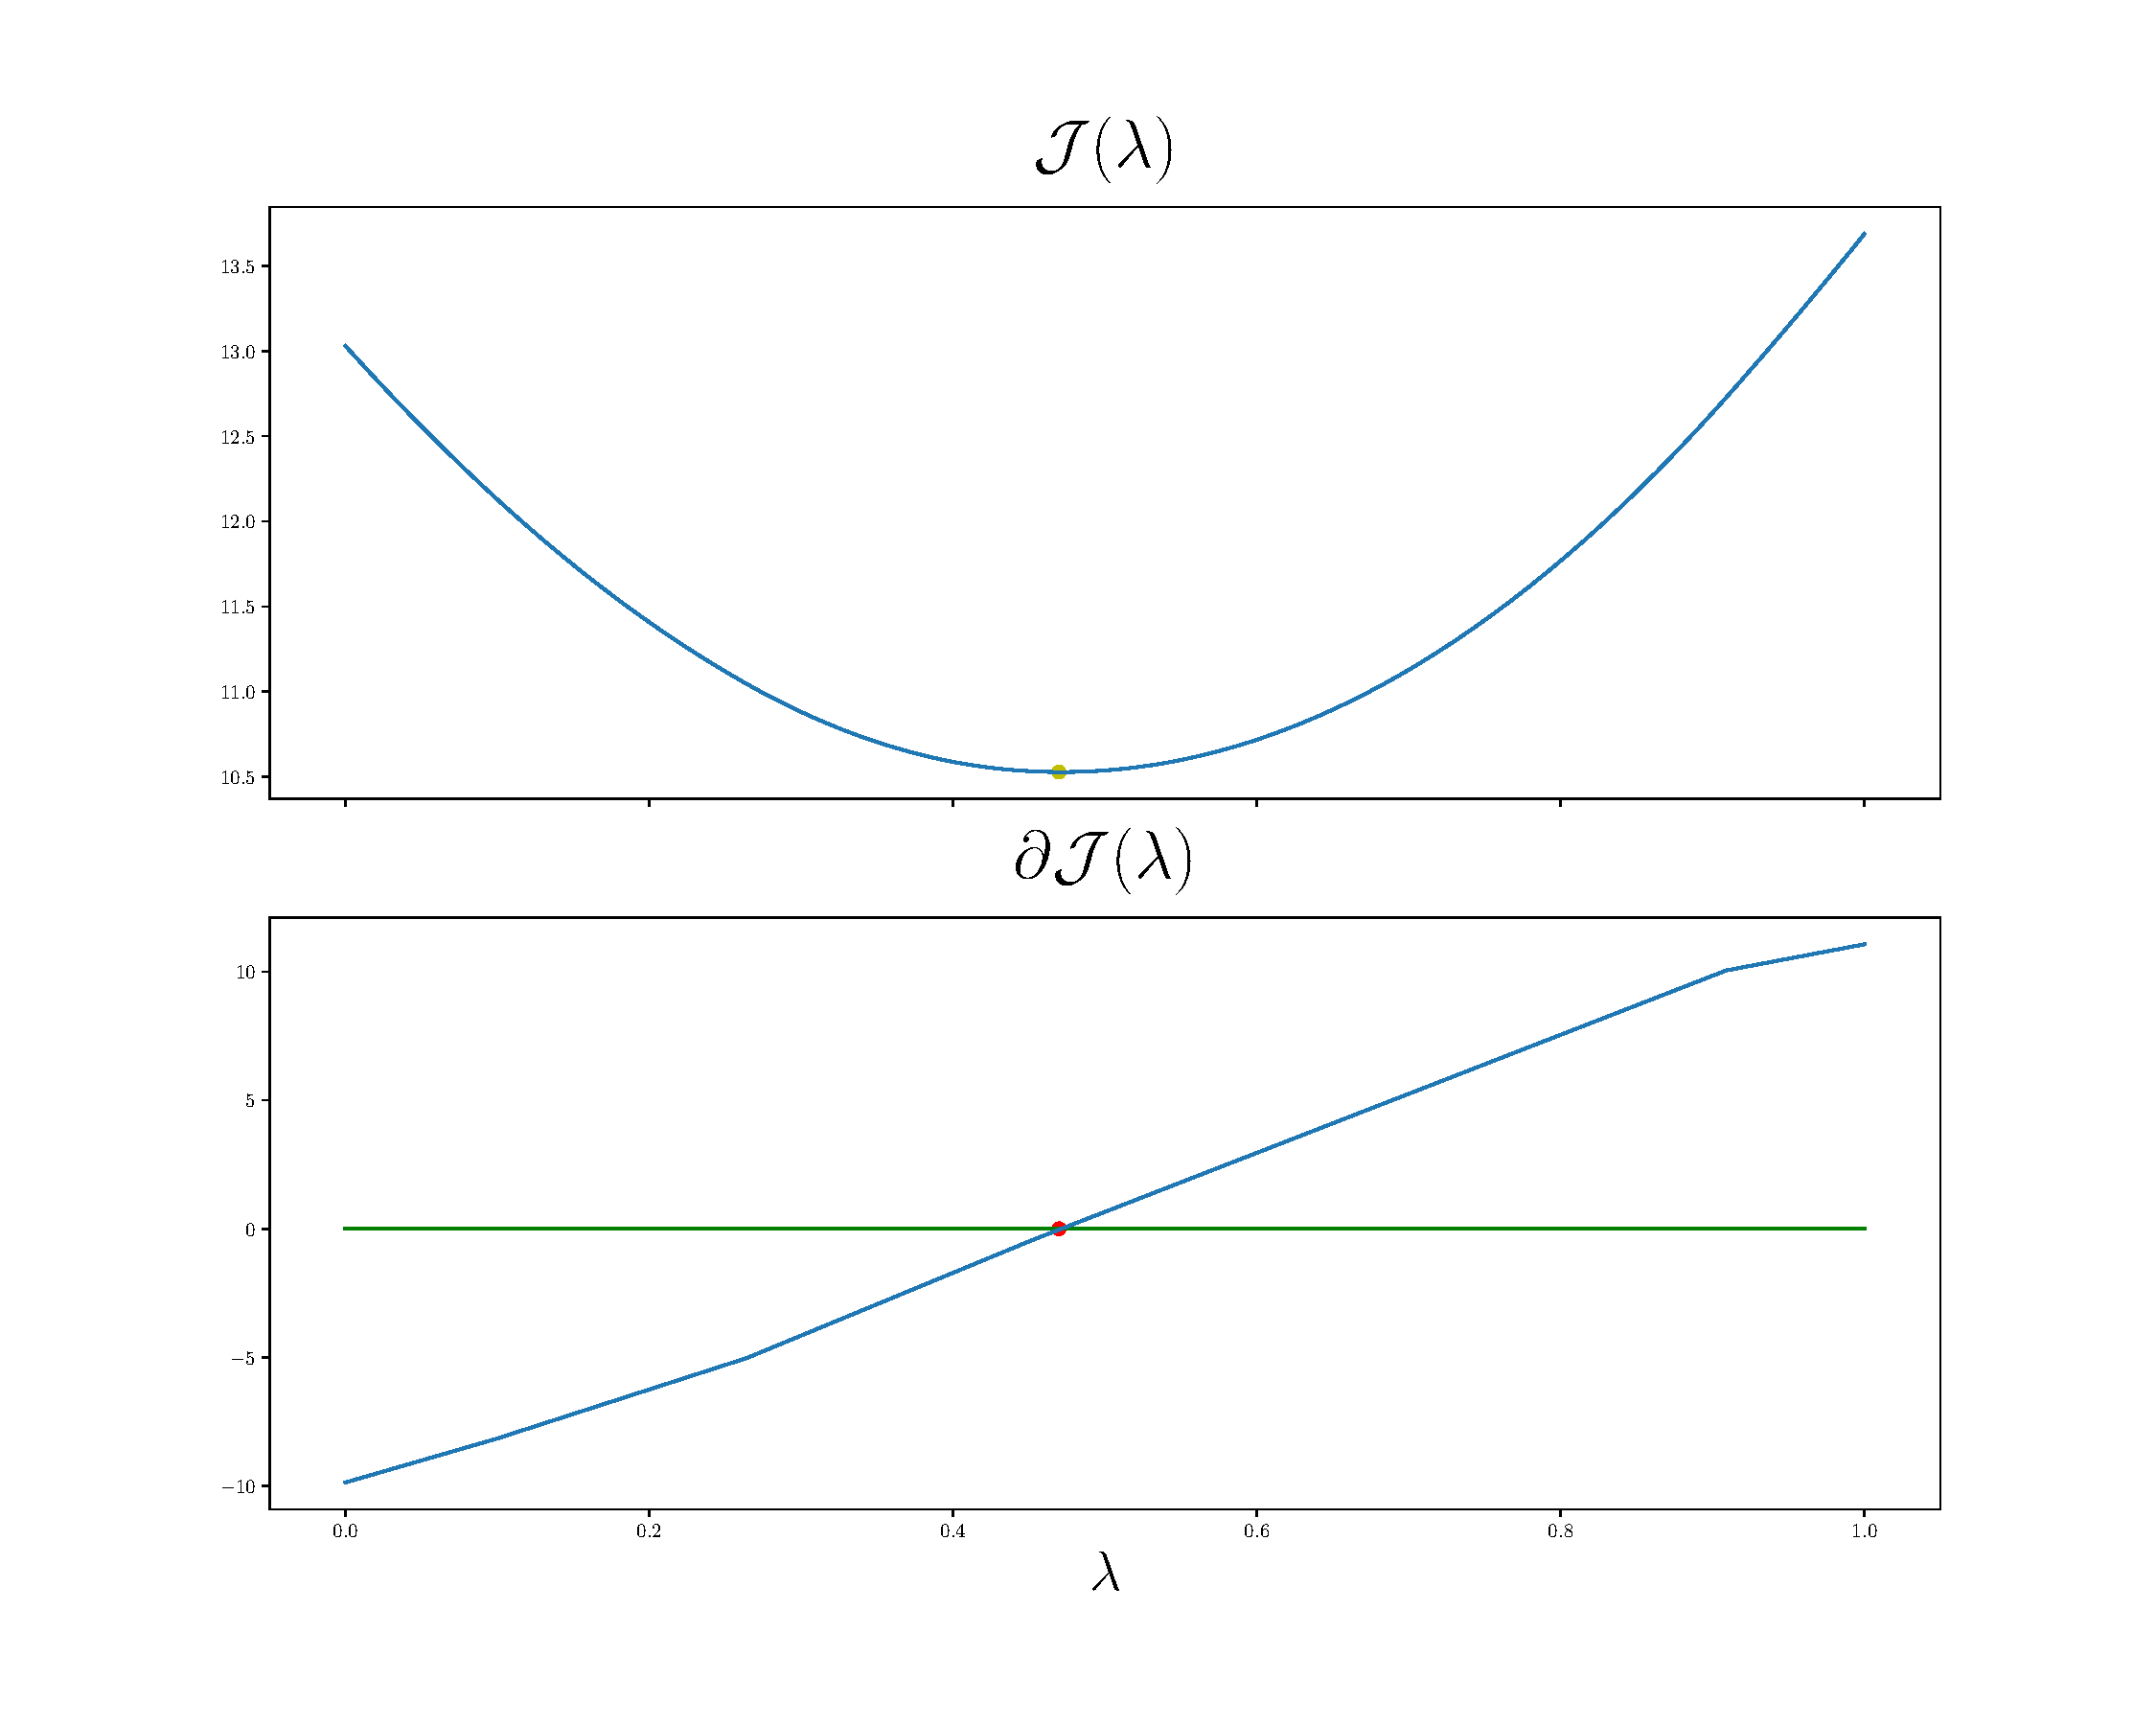
\includegraphics[width=\textwidth]{Chapter4/NeuroCom2021/ejemplo2_sqhinge.pdf}
    \caption{Error using squared hinge loss function (top) and its corresponding subgradient (bottom). The green line represents the $0$ constant function. The yellow dot is the point minimizing the error, and whose corresponding subgradient contains the value $0$.}
    \label{fig:sqhinge_error}
\end{figure}

As with the other losses, the error function and respective gradient for $10$ random pairs $(c_i, d_i)$ are represented in Figure~\ref{fig:sqhinge_error}.





\subsection{Experiments}\label{subsec:convexmtlsvm_exp}
In this subsection we show the experiments used to test the convex MTL formulation with kernel models, which have been presented in~\citep{RuizAD19} and~\citep{RuizAD21}. 
%
First, following the work in~\citep{RuizAD19}, experiments comparing convex and additive MTL formulations in the L1-SVM are described. 
%
Then, the experiments of~\citep{RuizAD21} are exposed, where all convex MTL models using L1, L2 and LS-SVMs as well as optimal convex combination of pre-trained models are compared using multiple real problems.

Before diving into the results, some technical details have to be explained. The convex MTL formulation, as presented in Equation~\eqref{eq:svmmtl_primal_convex}, uses task-specific hyperparameters $\lambda_r$, as well as common and task-specific kernels, with their corresponding hyperparameters; however, the selection of hyperparameters is always a challenge because of the curse of dimensionality. 
%
To select the hyperparameters $p_1, \ldots, p_L$ of a learning algorithm using CV the following problem is solved:
\begin{equation}
    \label{eq:hp-selection_general}
    p_1^*, \ldots, p_L^* = \argmin_{p_i \in \mathcal{S}_{p_i}, i=1, \ldots, L} \sum_{j=1}^{F} \rho(\mathcal{A}(p_1, \ldots, p_L; (X^j_\text{train}, y^j_\text{train})); (X^j_\text{val}, y^j_\text{val})) ,
\end{equation}
where $\rho$ is some measure, $\mathcal{A}$ is our choice of learning algorithm; $p_1, \ldots, p_L$ are the parameters on which $\mathcal{A}$ depends and $\mathcal{S}_{p_i}$ a feasible space for the parameter $p_i$; and $(X^j_\text{train}, y^j_\text{train}), (X^j_\text{val}, y^j_\text{val})$ are the training and validation sets, respectively. We are using $F$ folds, that is, for $j=1, \ldots, F$ we select different training and validation sets and we train our algorithm $\mathcal{A}$ on the training set $(X^j_\text{train}, y^j_\text{train})$, then we use $\rho$ to measure the wellness of our model on $(X^j_\text{val}, y^j_\text{val})$. 
%
Observe that our search space is the product space $\mathcal{S}_{p_1} \times \ldots \times \mathcal{S}_{p_L}$, so the difficulty of selecting an optimal combination of hyperparameters scales exponentially with the number of such parameters.

%
In a standard Gaussian kernel SVM, the definition of the problem depends on two hyperparameters: $C$ and $\gamma$.
In the L1 and L2-SVM for regression problems we also add a third parameter: $\epsilon$. 
That is, to select the hyperparameters of a standard SVM for a single task we have to solve the problem
\begin{equation}
    \nonumber
    C^*, \gamma^* (, \epsilon^*) = \argmin_{\substack{C \in \mathcal{S}_C ; \\ \substack{\gamma \in \mathcal{S}_\gamma} ; \\ \left(\substack{\epsilon \in \mathcal{S}_\epsilon} \right); }}
     \sum_{j=1}^{F} \rho(\mathcal{A}(C, \gamma (, \epsilon); (X^j_\text{train}, y^j_\text{train})); (X^j_\text{val}, y^j_\text{val})) ,
\end{equation}
which is typically feasible by using a grid search method in the space $\mathcal{S}_{C} \times \mathcal{S}_{\gamma} (\times \mathcal{S}_{\epsilon}) .$
%

However, using the convex MTL formulation, 
%as shown in the MTL kernel expression~\eqref{eq:conv_mtl_kernel_fun}, there are a common width $\gamma$ and task-specific widths $\gamma_1, \ldots, \gamma_\ntasks$.
we have the following hyperparameters: the regularization parameter $C$; the common kernel width $\gamma$, and task-specific ones $\gamma_1, \ldots, \gamma_\ntasks$; and the convex combination parameters $\lambda_1, \ldots, \lambda_\ntasks$; and possibly the $\epsilon$ parameter. That is, there are at least $2\ntasks + 2$ hyperparameters that have to be selected. Even with $\ntasks=2$, a search space of dimension $6$ is computationally unfeasible to cover.
% \begin{equation}
%     \nonumber
%     C^*, \gamma^*, \gamma_1^*, \ldots, \gamma_\ntasks^*, \lambda_1^*, \ldots, \lambda_\ntasks^*   (, \epsilon^*) = \argmin_{\substack{C \in \mathcal{S}_C ; \\ \substack{\gamma \in \mathcal{S}_\gamma} ; \\ \left(\substack{\epsilon \in \mathcal{S}_\epsilon} \right); }}
%      \sum_{j=1}^{F} \rho(\mathcal{A}(C, \gamma (, \epsilon); (X^j_\text{train}, y^j_\text{train})); (X^j_\text{val}, y^j_\text{val})) ,
% \end{equation}

To solve this difficulty and select the optimal parameters for the convex MTL formulation we follow the following strategy.
%
For the kernel widths, we proceed as follows: we first hyperparametrize the corresponding CTL and ITL kernel models, which have a common and task-specific kernel widths, respectively. 
Observe that in the CTL approach where a single virtual task is solved and in the ITL approach, where we solve the tasks independently, we have $2$ or $3$ parameters. We solve problems, which are represented in Equation~\eqref{eq:hp-selection_general}, using standard methods, and we obtain optimal common $C^*, \gamma^*$ and task-specific ones $C_r^*, \gamma^*_r$ for $r=1, \ldots, \ntasks$.
Then, we reutilize the optimal widths for these models, and fix them in the MTL one.
%
Moreover, for the convex combination parameters we use a single $\lambda$ for all tasks, that is, $\lambda_1 = \ldots = \lambda_\ntasks = \lambda$.
%
With these considerations, the problem to select the remaining hyperparameters is 
\begin{equation}
    \nonumber
    C^*, \lambda^* (, \epsilon^*) = \argmin_{\substack{C \in \mathcal{S}_C ; \\ \substack{\lambda \in \mathcal{S}_\lambda} ; \\ \left(\substack{\epsilon \in \mathcal{S}_\epsilon} \right); }}
     \sum_{j=1}^{F} \rho(\mathcal{A}(C, \lambda, \gamma^*, \gamma_1^*, \ldots, \gamma_\ntasks^* (, \epsilon); (X^j_\text{train}, y^j_\text{train})); (X^j_\text{val}, y^j_\text{val})) ,
\end{equation}
where we have a maximum of $3$ hyperparameters.

%
These are the two adjustments that we make to carry out the experiments shown in this subsection.
The first adjustment concerning kernel widths does not change the model definition, but it assumes that kernel widths that are good for CTL or ITL models are good for the MTL one. This assumption is a sensible one, since kernel widths are not that descriptive of the model but of the data used. The combined data from all tasks, which is used in CTL approach, is well ``characterized'' by a width $\sigma^*$ so we expect that this width is also useful for the common part of the MTL model. The same reasoning applies to task-specific data and ITL approach.
%
The second adjustment does change the models definition, using a single $\lambda$ that determines the specifity of all models. However, we expect that the possible difference in specifity among tasks can be corrected in the training process by selecting larger task-specific weights $v_r$ if necessary.

\paragraph*{Comparison of Convex and Additive Formulations.\\}
% Figure Synthetic Problem HAIS2019
\begin{figure}
    \centering
    \begin{subfigure}[b]{0.45\textwidth}
        \centering
        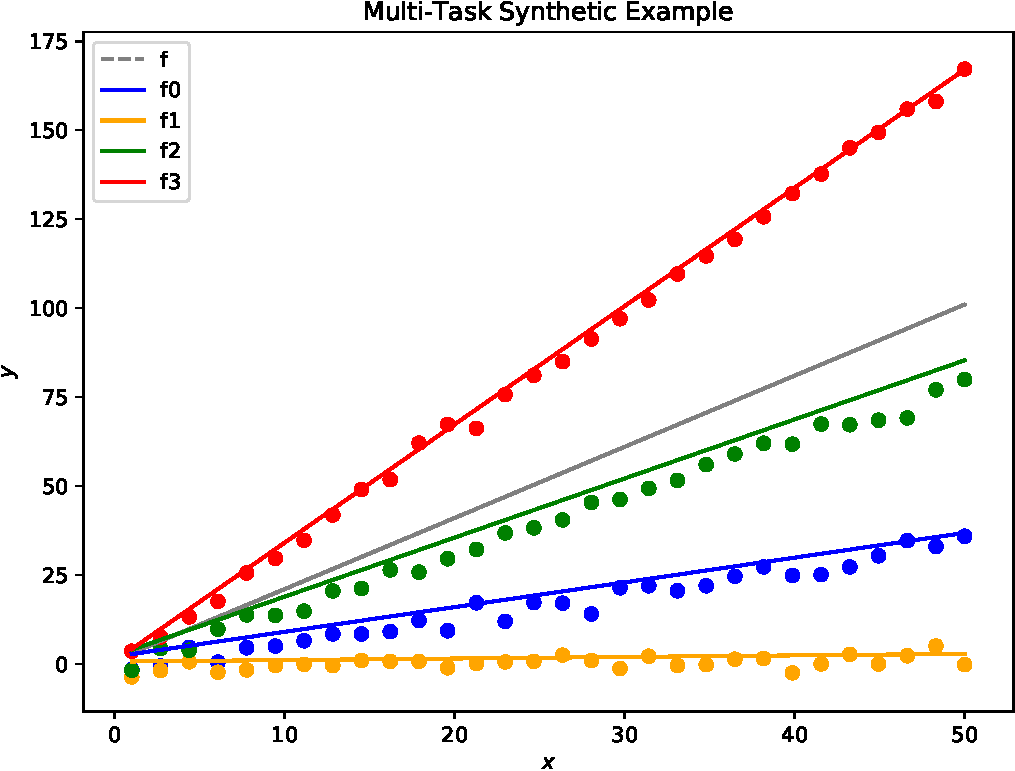
\includegraphics[width=\textwidth]{Chapter4/HAIS2019/synthetic_example-crop.pdf}
    \end{subfigure}
    \hfill
    \begin{subfigure}[b]{0.45\textwidth}
        \centering
        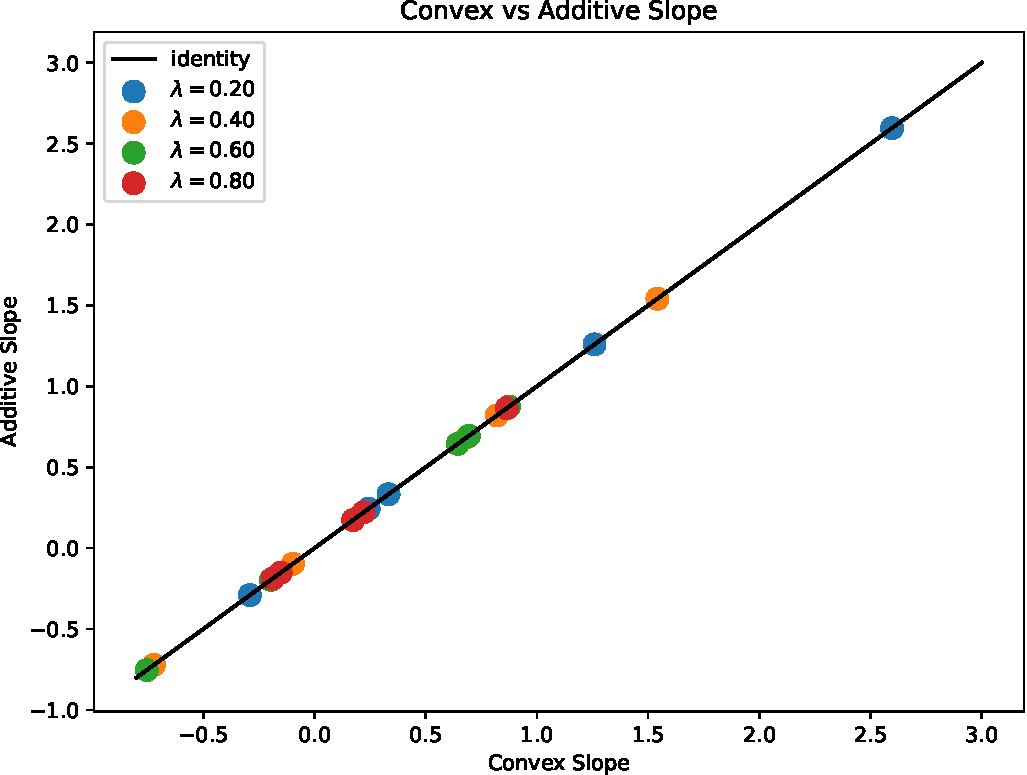
\includegraphics[width=\textwidth]{Chapter4/HAIS2019/synthetic_comparison-crop.pdf}
    \end{subfigure}
    \caption{Left: Synthetic example dataset, where the data of each task (corresponding to a different function $f_i$) are represented with a different color.
        Right: Comparison of the weights obtained by the {convex} and {additive} approaches.}
    \label{fig:lines_slopes}
\end{figure}

% Figure Convex vs Additive HAIS2019
\begin{figure}
    \centering
    \begin{subfigure}[b]{0.45\textwidth}
        \centering
        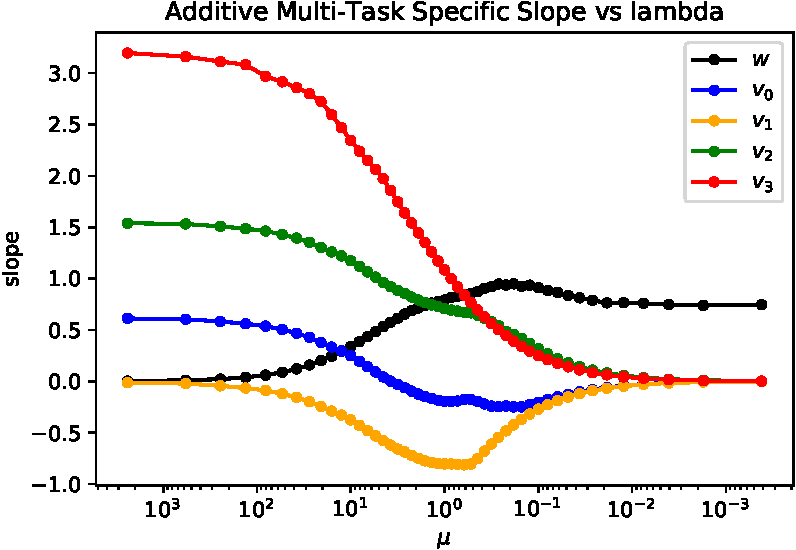
\includegraphics[width=\textwidth]{Chapter4/HAIS2019/synthetic_specWeights_add-crop.pdf}
    \end{subfigure}
    \hfill
    \begin{subfigure}[b]{0.45\textwidth}
        \centering
        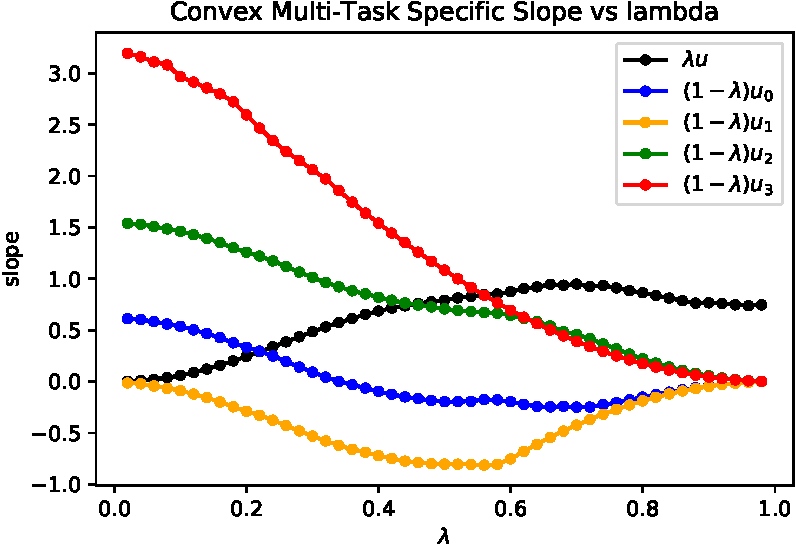
\includegraphics[width=\textwidth]{Chapter4/HAIS2019/synthetic_specWeights_conv-crop.pdf}
    \end{subfigure}
    \caption{{Convex} (right) and {additive} (left) MTLSVR slope estimates weights as a function of $\lambda$. We represent the common part of the models, $w$ for the {additive} and $\lambda u$ for the {convex}, as well as each task specific deviation $v_t$ and $(1 - \lambda) u_t$.}
    \label{fig:synthetic_specWeights}
\end{figure}

%The work shown in~\cite{RuizAD19} focuses on 

In~\citep{RuizAD19}, we illustrate the results of equivalence between the additive and convex formulations in an empirical way. To do this we generate a synthetic problem, shown in Figure~\ref{fig:lines_slopes}, left, as a four linear regression tasks problem. 
%
We use four different functions $f_0, f_1, f_2, f_3$ by considering a base function $f(x) = 2x - 1$ with slope $m=2$ and bias $n=1$, then we sample $z_m^r, z_n^r \sim \normal{0, 1}$ for each task $r=0, \ldots, 3$ and create the $r$-th slope and bias by adding these Gaussian samples, i.e., $m_r = m + z_m^r$ and $n_r = n + z_n^r$. Also, we sample the noise $\sigma_r$ for each task uniformly in $(0, 5)$. 
%
Then, the $r$-th task consists on estimating $m_r$ and $n_r$ from data. To do this, for each task we uniformly sample $30$ points $x_i^r \in [1, 50)$, and the target values are defined as $y_i^r = f_r(x_i^r) + \epsilon^i_r$ where $\epsilon^i_r \sim \normal{0, \sigma_r}$.
%
Combining all tasks, there are $120$ data points, $30$ for each task, that we split randomly in a stratified way: two thirds, i.e. $80$ points are used for training, and the rest are used for testing purposes; in this division, the task size proportions are kept constant, that is $1/4$ for each task, in both the train and test sets. 
%
With this synthetic problem, we train four convex MTL models corresponding to values of $\lambda \in \set{0.2, 0.4, 0.6, 0.8}$; and we also train the corresponding equivalent additive MTL models, in which we set $\mu = (1 - \lambda)/\lambda^2$ and $C_\text{add} = (1 - \lambda)^2 C_\text{conv}$, as shown in Proposition~\ref{prop:add_conv_equiv}.
%
Our goal is to compare the influence of $\mu$ with that of $\lambda$ in the final models that are obtained. To do that, we need $C$ to be small enough so the regularization and, therefore, $\mu$ are relevant; the value $C_{\text{conv}} = 10^{-2}$ is found to be useful. We also consider linear kernels, so we can obtain the primal coefficients, that is, the slopes, and compare those obtained using the additive and convex formulations. In Figure~\ref{fig:lines_slopes}, right, we show the estimated slopes for each of the $\lambda$ values considered with a different color. In the $x$ axis we represent the convex slopes and in the $y$ axis the additive ones. There are four dots of each color, corresponding to each of the tasks considered in our synthetic problem. We can observe that all dots lie in the diagonal line corresponding to the identity function, as we expected from the equivalence result from Proposition~\ref{prop:add_conv_equiv}.

%
To further compare the two formulations, to visualize how the change on the hyperparameters imposes a change on the final models. Using the already described synthetic problem of Figure~\ref{fig:lines_slopes}, left, we select values of $\lambda$ ranging from $0$ to $1$, and their corresponding values $\mu = (1-\lambda)^2 / \lambda^2$, and fit convex and additive MTL linear SVMs using these values. In Figure~\ref{fig:synthetic_specWeights} we show the coefficients obtained for the common and task-specific parts with the additive formulation (left) and convex one (right).
%
We can observe how both graphics show a similar behaviour, with the common model starting in $0$ when $\mu$ is large or $\lambda=0$, and, as $\mu$ decreases and $\lambda$ grow, the task-specific parts go to zero and the common model reaches the optimal value for CTL.
%
However, two facts are noticeable, the first one is the range of hyperparameters needed for each formulation; while the convex formulation always uses $[0, 1]$, with the additive formulation it seems that $(10^{-3}, 10^3)$ is useful in this problem, but we cannot extrapolate to other problems; the second one is the smoother transition of the convex formulation, where the changes are steadily made, while with the additive one the changes look more abrupt.



\paragraph*{Performance of Convex MTL and Optimal Convex Combination.\\}

To test the performance of the convex MTL formulation, in~\citep{RuizAD19} we also conduct experiments with real problems, which are extended in~\citep{RuizAD21}. 
% Models
\paragraph*{Models.}
Considering that {LX} can stand for {L1}, {LS} or {LS}, we use the following approaches:
\begin{itemize}
    \item {Common Task Learning LX-SVM (\fmod{CTL-LX})}: A single LX-SVM which is fitted using data from all the tasks and does not use of the task information.
    \item {Independent Task Learning LX-SVM (\fmod{ITL-LX})}: Multiple task-specific LX-SVMs, each of which is fitted with the data from its own task.
    \item {Direct Convex Combination of LX-SVMs (\fmod{cvxCMB-LX})}: A combination of the best \fmod{CTL-LX} and \fmod{ITL-LX} as described in Subsection~\ref{subsec:optimal_comb}.
    \item {Convex Multi-Task Learning LX-SVM (\fmod{cvxMTL-LX})}: The Convex MTL formulations shown in Subsection~\ref{subsec:cvx_l1-svm} for the L1-SVM and in Subsection~\ref{subsec:cvx_l2ls-svm} for the L2- and LS-SVM.
\end{itemize}

% Problems
\paragraph*{Problems.}
To compare these approaches we will use several regression and classification problems. We use a total of six regression problems:
\begin{itemize}
    \item \fdata{majorca}: The goal is to predict the photovoltaic energy production of a park installed in Mallorca. The tasks are defined as the energy prediction at each hour with sunlight (we remove the night hours).
    \item \fdata{tenerife}: The goal is to predict the photovoltaic energy production of a park installed in Tenerife. The tasks are defined as the energy prediction at each hour with sunlight (we remove the night hours).
    \item \fdata{boston}: This is the housing problem in Boston, where the goal is to predict house prices, and the tasks are defined as the predictions in different areas of the city. In Boston we have the houses that are next to the river and those that are not.
    \item \fdata{california}: This is the housing problem in California, where the goal is also to predict house prices. Here the tasks correspond to 4 different areas of the city, related to their distance to the sea.
    \item \fdata{abalone}: The goal is to predict the number of rings of a specie of marine molluscs. The tasks are male, female or infant.
    \item \fdata{crime}: The goal is to predict the number of crimes per $100.000$ habitants in the U.S., the tasks are the prediction of the crime rate in different states.
\end{itemize}
For the classification setting, we consider eight problems, six of which are generated by applying different task definitions to two different problems.
\begin{itemize}
    \item \fdata{landmine}: This is a binary classification problem in which the goal is to detect landmines. Detection of different types of landmines determines a different task each. 
    \item \fdata{binding}: This is a binary classification problem where the goal is to determine if a given molecule will bind peptides. Different molecules define different tasks.
    \item \fdata{adult}: The goal is to predict whether the salary of a particular person is greater than 50K based on sociocultural data. We can define different tasks dividing the population by either gender or race, so we have the problems:
    \begin{itemize}
        \item \fdata{ad\_\{G\}}: dividing by gender
        \item \fdata{ad\_\{R\}}: dividing by race
        \item \fdata{ad\_\{G, R\}}: dividing by both gender and race
    \end{itemize}
    \item \fdata{compas}: The goal is to predict whether the COMPAS algorithm will assign "low" or "high" scores of recidivism to a particular subject. We can also divide the sample by either race or gender, so we obtain:
    \begin{itemize}
        \item \fdata{comp\_\{G\}}: dividing by gender
        \item \fdata{comp\_\{R\}}: dividing by race
        \item \fdata{comp\_\{G, R\}}: dividing by both gender and race
    \end{itemize}
\end{itemize}
The characteristics of some of the problems considered are present in Table~\ref{tab:mtl_problems} but, considering the different task definitions for \fdata{compas} and \fdata{adult} we give a more complete table in Table~\ref{tab:problems_hais19}.

% Table Problems HAIS19
\begin{table*}[t!]
    \caption{Sample sizes, dimensions and number of tasks of the datasets used.}
    \label{tab:problems_hais19}
    \centering
    \scalebox{.65}{
    \begin{tabular}{l*{7}{S[table-format=5]}}
    \toprule
    \fhead{Dataset} & \fhead{Size} & \fhead{No. feat.} & \fhead{No. tasks} & \fhead{Avg. task size} & \fhead{Min. t. s.} & \fhead{Max. t. s.}\\
    \midrule
    \fdata{majorca} & 15330 & 765 & 14 & 1095 & 1095 & 1095 \\ 
    \fdata{tenerife} & 15330 & 765 & 14 & 1095 & 1095 & 1095 \\
    \fdata{california} & 19269 & 9 & 5 & 3853 & 5 & 8468\\
    \fdata{boston} & 506 & 12 & 2 & 253 & 35 & 471 \\
    \fdata{abalone} & 4177 & 8 & 3 & 1392 & 1307 & 1527 \\
    \fdata{crime} & 1195 & 127 & 9 & 132 & 60  & 278 \\
    \fdata{binding} & 32302 & 184 & 47 & 687 & 59 & 3089 \\ 
    \fdata{landmine} & 14820 & 10 & 28 & 511 & 445 & 690 \\
    \fdata{adult\_(G)} & 48842 & 106 & 2 & 24421 & 16192 & 32650 \\
    \fdata{adult\_(R)} & 48842 & 103 & 5 & 9768 & 406 & 41762 \\
    \fdata{adult\_(G, R)} & 48842 & 101 & 10 & 4884 & 155 & 28735 \\
    \fdata{compas\_(G)} & 3987 & 11 & 2 & 1993 & 840 & 3147 \\
    \fdata{compas\_(R)} & 3987 & 9 & 4 & 997 & 255 & 1918 \\
    \fdata{compas\_(G, R)} & 3987 & 7 & 8 & 498 & 50 & 1525 \\
    \bottomrule
   \end{tabular}}
\end{table*}

% Experimental Procedure

% Table Hyperparameters HAIS19
\begin{table}[t]
    \caption{Hyperparameters, grids used to select them (when appropriate) and hyperparameter selection method for each model.}
    \label{tab:hyperpars_grid}
    \centering
    \scalebox{.65}{
     \begin{tabular}{*{9}{c}}
     \toprule
     \fhead{} & \fhead{Grid} & \fhead{\fmod{CTL-L1,2}} & \fhead{\fmod{ITL-L1,2}} & \fhead{\fmod{cvxMTL-L1,2}}  & \fhead{\fmod{CTL-LS}} & \fhead{\fmod{ITL-L,S}} & \fhead{\fmod{cvxMTL-LS}}   \\
     \midrule
      $C$ &  \scalebox{.9}{$\set{4^k: -2 \leq k \leq 6}$} & CV & CV & CV & CV & CV & CV  \\ 
      $\epsilon$ & \scalebox{.9}{$\set{\frac{\sigma}{4^k}: 1 \leq k \leq 6}$} & CV & CV & CV & - & - & - \\
      $\gamma_c$ & \scalebox{.9}{$\set{\frac{4^k}{d}: -2 \leq k \leq 3}$} & CV & - & \fmod{CTL-L1,2} & CV & - & \fmod{CTL-LS} \\
      $\gamma_s^r$ & \scalebox{.9}{$\set{\frac{4^k}{d}: -2 \leq k \leq 3}$} & - & CV & \fmod{ITL-L1,2} & - & CV & \fmod{ITL-LS}\\
      $\lambda$ & \scalebox{.9}{$\set{0.1 k : 0 \leq k \leq 10}$} & - & - & CV & - & - & CV \\
      \bottomrule
     \end{tabular}
     }
  \end{table}

\paragraph*{Experimental Procedure.}
To obtain the experimental results, we have to select the optimal hyperparameters for each model in a training-validation set and measure its performance on a test set. To do this, we follow the adjustments and experimental procedure described at the beginning of this subsection: reusing the kernel widths from CTL and ITL approaches and limiting the convex MTL formulation to a single parameter $\lambda$.
%
In all models considered we use Gaussian kernels, so all features have been scaled to the $[0, 1]$ interval.
As previously explained, the hyperparameters for the CTL and ITL approaches in the classification setting are $\set{C, \gamma}$ for all variants L1, L2 and LS-SVM.
In the regression setting we have $\set{C, \gamma, \epsilon}$ for the L1 and L2 variants, and $\set{C, \gamma}$ for the LS-SVM.
%
After selecting the optimal kernel widths in the CTL approach $\sigma^*$, and the task-specific widths $\sigma_r^*$ in the ITL approach, we use these values to fix them in the convex MTL formulation.
Then, the hyperparameters that we are considering for CV search in the convex MTL approaches in the classification settings are $\set{C, \lambda}$ for all variants, while in the regression problems they are $\set{C, \lambda, \epsilon}$ for the L1 and L2 variants and $\set{C, \lambda}$ for the LS-SVM.
%
The optimal combination approaches do not have proper hyperparameters, since $\lambda$ can be considered a training parameter.
%
In all problems, the hyperparameters considered are selected with a grid search using a task-stratified $3$-fold CV. That is, given a training-validation set, we divide it in three different folds where the task proportions are kept constant, and we use two of these folds for training the model and evaluate its performance in the remaining one.
%
In the regression problems, we will measure the validation performance using the MAE, see Table~\ref{tab:error_models_reg_mae_mae}, and MSE, see Table~\ref{tab:error_models_reg_mse_mae}.  Observe that the objective function of L1-SVM based models is more aligned with minimizing the MAE, while those of L2 and LS-SVM based models are more related to minimizing the MSE.
In the classification problems, see Table~\ref{tab:error_models_class_f1}, we will consider the F1 score to deal with the class-imbalance ratio that we find, for example, in the \fdata{landmine} dataset where we have 200 negative examples for every 13 positive ones.
%
In Table~\ref{tab:hyperpars_grid} we show for each hyperparameter of the considered approaches if they are selected using a CV procedure or recycling them from other approach, as well as the grids used for the CV search.

We have explained how we select the hyperparameters given a training-validation set, but it is necessary also to describe how we get the final results that we show on tables.
In every problem, except for \fdata{majorca} and \fdata{tenerife}, we will consider three external folds, each with the internal three folds for cross-validation. That is, the whole dataset of each problem is first divided in three task-stratified external folds: $F_1, F_
2, F_3$; then, two folds will form the training-validation set and the third one will be used as the test set. All folds have the same task proportions. There are three different combinations to do this division: $\set{F_1, F_2; F_3}, \set{F_1, F_3; F_2}$ and $\set{F_2, F_3; F_1}$, where the first two folds form the train-validation set and the other one is the test set.
%
In each train-validation set we follow the procedure described above to select the optimal hyperparameters, and the performance model with the optimal hyperparameters will be tested in the remaining fold, i.e., the test set.
%

The problems of \fdata{majorca} and \fdata{tenerife} have a temporal dependency, so it is not possible to use training data from a time that is ahead of that of the test or validation data. Therefore, we use data from years 2013, 2014 and 2015, each corresponding to train, validation and test sets, respectively.
%
We consider different metrics to measure the test performance. Therefore, in every problem, except \fdata{majorca} and \fdata{tenerife}, for each metric we obtain three different scores, each corresponding to a different test set, so we will show the mean and standard deviation of such scores. In \fdata{majorca} and \fdata{tenerife} we obtain a single test score corresponding to data from the year 2015.
% 
For the regression problems, in Tables~\ref{tab:error_models_reg_mae_mae} and~\ref{tab:error_models_reg_mse_mae}, we show both the MAE and R2 score, closely related to MSE, obtained in the test set, and for classification, in Table~\ref{tab:error_models_class_f1}, we show the F1 and the accuracy scores.
%




% Results


  \begin{table*}[t]
    \captionsetup{font=scriptsize}
    \caption{Test MAE (top) and R2 score (bottom) and Wilcoxon-based ranking for the models selected using the MAE for hyperparametrization. The best models are shown in bold.}
    \label{tab:error_models_reg_mae_mae}
    \centering
    \scalebox{.65}{
    \begin{tabular}{l*{2}{c@{ }l}*{4}{r@{$\pm$}l@{ }l } }
    \toprule
    & \fheadmulti{2}{\fdata{maj.}} & \fheadmulti{2}{\fdata{ten.}} & \fheadmulti{3}{\fdata{boston}} & \fheadmulti{3}{\fdata{california}} &  \fheadmulti{3}{\fdata{abalone}} & \fheadmulti{3}{\fdata{crime}}\\
    \midrule
    & \fheadmulti{16}{MAE} \\
    \midrule
    \fmod{ITL-L1}            &  {5.087} &   (6) &  {5.743} &   (3) &  {2.341} & {0.229} &   \fmaxn{(1)} &  {36883.582} & {418.435} &   (2) &  {1.481} & {0.051} &   (3) &  {0.078} & {0.001} &   (2) \\
    \fmod{CTL-L1}            &  {5.175} &   (7) &  {5.891} &   (5) &  \fmaxn{2.192} & \fmaxn{0.244} &   \fmaxn{(1)} &  {41754.337} & {270.908} &   (6) &  {1.482} & {0.050} &   (3) &  {0.078} & {0.001} &   (2) \\
    \fmod{cvxCMB-L1} &  \fmaxn{5.047} &   (5) &  \fmaxn{5.340} &  \fmaxn{(1)} &  {2.239} & {0.255} &   \fmaxn{(1)} &  {36880.238} & {420.417} &   \fmaxn{(1)} &  {1.470} & {0.052} &   (2) &  {0.077} & {0.002} &   (2) \\
    \fmod{cvxMTL-L1}     &  {5.050} &   (5) &  {5.535} &   (2) &  {2.206} & {0.292} &   \fmaxn{(1)} &  \fmaxn{36711.383} & \fmaxn{343.333} &  \fmaxn{(1)} &  \fmaxn{1.454} & \fmaxn{0.048} &  \fmaxn{(1)} &  \fmaxn{0.074} & \fmaxn{0.002} &  \fmaxn{(1)} \\
    \midrule
    \fmod{ITL-L2}            &  {4.952} &   (3) &  \fmaxn{5.629} &   (3) &  {2.356} & {0.300} &   \fmaxn{(1)} &  {37374.618} & {433.511} &   (5) &  {1.498} & {0.054} &   (4) &  {0.079} & {0.002} &   (2) \\
    \fmod{CTL-L2}            &  {5.193} &   (7) &  {6.107} &   (8) &  \fmaxn{2.083} & \fmaxn{0.136} &   \fmaxn{(1)} &  {42335.612} & {163.773} &   (8) &  {1.503} & {0.047} &   (5) &  {0.080} & {0.002} &   (2) \\
    \fmod{cvxCMB-L2} &  {4.869} &   (3) &  {5.963} &   (6) &  {2.089} & {0.128} &   \fmaxn{(1)} &  {37374.618} & {433.511} &   (4) &  {1.494} & {0.050} &   (4) &  {0.077} & {0.003} &   (2) \\
    \fmod{cvxMTL-L2}     &  \fmaxn{4.854} &   (2) &  {5.784} &   (4) &  {2.089} & {0.134} &   \fmaxn{(1)} &  \fmaxn{37202.603} & \fmaxn{419.166} &   (3) &  \fmaxn{1.482} & \fmaxn{0.049} &   (3) &  \fmaxn{0.077} & \fmaxn{0.002} &   (2) \\
    \midrule
    \fmod{ITL-LS}            &  {4.937} &   (3) &  {5.649} &   (3) &  {2.204} & {0.116} &   \fmaxn{(1)} &  {37348.347} & {441.240} &   (4) &  {1.496} & {0.051} &   (4) &  {0.079} & {0.002} &   (2) \\
    \fmod{CTL-LS}            &  {5.193} &   (7) &  {6.005} &   (7) &  \fmaxn{2.072} & \fmaxn{0.143} &  \fmaxn{(1)} &  {42259.492} & {146.825} &   (7) &  {1.502} & {0.052} &   (5) &  {0.079} & {0.002} &   (2) \\
    \fmod{cvxCMB-LS} &  {4.977} &   (4) &  \fmaxn{5.593} &   (3) &  {2.081} & {0.146} &   \fmaxn{(1)} &  {37339.179} & {430.288} &   (4) &  {1.486} & {0.049} &   (4) &  {0.079} & {0.002} &   (2) \\
    \fmod{cvxMTL-LS}     &  \fmaxn{4.824} &  \fmaxn{(1)} &  {5.754} &   (4) &  {2.077} & {0.152} &   \fmaxn{(1)} &  \fmaxn{37231.043} & \fmaxn{420.992} &   (4) &  \fmaxn{1.478} & \fmaxn{0.050} &   (3) &  \fmaxn{0.076} & \fmaxn{0.002} &   (2) \\
    \midrule
    & \fheadmulti{16}{R2} \\
    \midrule
    \fmod{ITL-L1}            &  {0.845} &   (6) &  {0.901} &   (7) &  {0.821} & {0.041} &   (2) &  {0.699} & {0.009} &   (7) &  {0.543} & {0.022} &   (8) &  {0.732} & {0.021} &   (3) \\
    \fmod{CTL-L1}            &  {0.837} &   (9) &  {0.901} &   (6) &  {0.854} & {0.036} &   \fmaxn{(1)} &  {0.639} & {0.006} &  (10) &  {0.559} & {0.014} &   (6) &  {0.740} & {0.027} &   (3) \\
    \fmod{cvxCMB-L1} &  {0.844} &   (6) &  {0.905} &   (4) &  {0.845} & {0.053} &   \fmaxn{(1)} &  {0.699} & {0.009} &   (6) &  {0.555} & {0.018} &   (7) &  {0.741} & {0.029} &   (3) \\
    \fmod{cvxMTL-L1}     &  \fmaxn{0.846} &   (4) &  \fmaxn{0.908} &   (2) &  \fmaxn{0.858} & \fmaxn{0.057} &   \fmaxn{(1)} &  \fmaxn{0.703} & \fmaxn{0.007} &   (6) &  \fmaxn{0.568} & \fmaxn{0.012} &   (5) &  \fmaxn{0.760} & \fmaxn{0.024} &   (2) \\
    \midrule
    \fmod{ITL-L2}            &  {0.846} &   (5) &  {0.906} &   (3) &  {0.836} & {0.045} &   (2) &  {0.707} & {0.009} &   (5) &  {0.565} & {0.025} &   (6) &  {0.743} & {0.017} &   (3) \\
    \fmod{CTL-L2}            &  {0.840} &   (8) &  {0.901} &   (8) &  \fmaxn{0.889} & \fmaxn{0.017} &   \fmaxn{(1)} &  {0.645} & {0.005} &   (9) &  {0.574} & {0.013} &   (4) &  {0.744} & {0.028} &   (3) \\
    \fmod{cvxCMB-L2} &  {0.850} &   (3) &  {0.900} &   (9) &  {0.885} & {0.013} &   \fmaxn{(1)} &  {0.707} & {0.009} &   (4) &  {0.571} & {0.018} &   (4) &  {0.755} & {0.024} &   (3) \\
    \fmod{cvxMTL-L2}     &  \fmaxn{0.863} &   (2) &  \fmaxn{0.908} &   \fmaxn{(1)} &  {0.888} & {0.015} &   \fmaxn{(1)} &  \fmaxn{0.709} & \fmaxn{0.008} &  \fmaxn{(1)} &  \fmaxn{0.580} & \fmaxn{0.014} &   (3) &  \fmaxn{0.762} & \fmaxn{0.028} &   \fmaxn{(1)} \\
    \midrule
    \fmod{ITL-LS}            &  {0.849} &   (3) &  {0.907} &   (3) &  {0.856} & {0.008} &   \fmaxn{(1)} &  {0.707} & {0.009} &   (3) &  {0.573} & {0.015} &   (4) &  {0.743} & {0.022} &   (3) \\
    \fmod{CTL-LS}            &  {0.838} &   (9) &  {0.904} &   (5) &  \fmaxn{0.894} & \fmaxn{0.015} &  \fmaxn{(1)} &  {0.646} & {0.005} &   (8) &  {0.576} & {0.016} &   (4) &  {0.746} & {0.032} &   (3) \\
    \fmod{cvxCMB-LS} &  {0.843} &   (7) &  {0.907} &   (2) &  {0.886} & {0.024} &   \fmaxn{(1)} &  {0.707} & {0.009} &   (2) &  {0.581} & {0.012} &   (2) &  {0.746} & {0.021} &   (3) \\
    \fmod{cvxMTL-LS}     &  \fmaxn{0.863} &  \fmaxn{(1)} &  \fmaxn{0.910} &  \fmaxn{(1)} &  {0.890} & {0.016} &   \fmaxn{(1)} &  \fmaxn{0.709} & \fmaxn{0.008} &   (2) &  \fmaxn{0.581} & \fmaxn{0.015} &  \fmaxn{(1)} &  \fmaxn{0.763} & \fmaxn{0.028} &  \fmaxn{(1)} \\
    \bottomrule
    \end{tabular}}
  \end{table*}





  \begin{table*}[t]
    \captionsetup{font=scriptsize}
    \caption{Test MAE (top) and R2 score (bottom) and Wilcoxon-based ranking for the models selected using the MSE for hyperparametrization. The best models are shown in bold.}
      \label{tab:error_models_reg_mse_mae}
      \centering
      \scalebox{.65
      }{
          \begin{tabular}{l*{2}{c@{ }l}*{4}{r@{$\pm$}l@{ }l } }
              \toprule
              & \fheadmulti{2}{\fdata{maj.}} & \fheadmulti{2}{\fdata{ten.}} & \fheadmulti{3}{\fdata{boston}} & \fheadmulti{3}{\fdata{california}} &  \fheadmulti{3}{\fdata{abalone}} & \fheadmulti{3}{\fdata{crime}}\\
      \midrule
      & \fheadmulti{16}{MAE} \\
      \midrule
      \fmod{ITL-L1}            &  {5.087} &   (7) &  {5.743} &   (3) &  {2.437} & {0.281} &   (3) &  {36941.516} & {450.767} &   (1) &  {1.480} & {0.058} &   (3) &  {0.079} & {0.002} &   (3) \\
      \fmod{CTL-L1}            &  {5.175} &   (8) &  {5.891} &   (7) &  {2.315} & {0.192} &   (2) &  {41857.602} & {235.021} &   (6) &  {1.479} & {0.047} &   (3) &  {0.078} & {0.000} &   (2) \\
      \fmod{cvxCMB-L1} &  \fmaxn{4.920} &   (4) &  {5.743} &   (4) &  {2.315} & {0.192} &   (3) &  \fmaxn{36941.476} & \fmaxn{450.711} &  \fmaxn{(1)} &  {1.471} & {0.057} &   (2) &  {0.079} & {0.002} &   (2) \\
      \fmod{cvxMTL-L1}     &  {5.050} &   (6) &  \fmaxn{5.535} &  \fmaxn{(1)} &  \fmaxn{2.244} & \fmaxn{0.150} &   (1) &  {36999.003} & {360.445} &   (2) &  \fmaxn{1.455} & \fmaxn{0.046} &  \fmaxn{(1)} &  \fmaxn{0.074} & \fmaxn{0.001} &  \fmaxn{(1)} \\
      \midrule
      \fmod{ITL-L2}            &  {4.924} &   (5) &  {5.752} &   (5) &  {2.437} & {0.324} &   (3) &  {37407.929} & {461.878} &   (5) &  {1.497} & {0.050} &   (5) &  {0.079} & {0.002} &   (2) \\
      \fmod{CTL-L2}            &  {5.193} &   (8) &  {6.107} &   (9) &  {2.096} & {0.112} &   (1) &  {42335.612} & {163.773} &   (7) &  {1.504} & {0.048} &   (6) &  {0.079} & {0.002} &   (2) \\
      \fmod{cvxCMB-L2} &  \fmaxn{4.813} &  \fmaxn{(1)} &  \fmaxn{5.623} &   (3) &  {2.116} & {0.131} &   (1) &  {37398.940} & {449.498} &   (5) &  {1.495} & {0.051} &   (5) &  {0.078} & {0.003} &   (2) \\
      \fmod{cvxMTL-L2}     &  {4.854} &   (4) &  {5.784} &   (6) &  \fmaxn{2.082} & \fmaxn{0.130} &   (1) &  \fmaxn{37356.599} & \fmaxn{390.629} &   (4) &  \fmaxn{1.481} & \fmaxn{0.041} &   (4) &  \fmaxn{0.076} & \fmaxn{0.000} &   (2) \\
      \midrule
      \fmod{ITL-LS}            &  {4.937} &   (5) &  {5.649} &   (3) &  {2.326} & {0.231} &   (3) &  {37385.244} & {403.331} &   (4) &  {1.495} & {0.045} &   (5) &  {0.079} & {0.002} &   (2) \\
      \fmod{CTL-LS}            &  {5.193} &   (8) &  {6.005} &   (8) &  \fmaxn{2.072} & \fmaxn{0.143} &  \fmaxn{(1)} &  {42339.063} & {156.624} &   (7) &  {1.504} & {0.043} &   (6) &  {0.078} & {0.002} &   (2) \\
      \fmod{cvxCMB-LS} &  \fmaxn{4.820} &   (2) &  {5.578} &   (2) &  {2.136} & {0.106} &   (1) &  {37377.005} & {391.694} &   (4) &  {1.491} & {0.048} &   (5) &  {0.078} & {0.002} &   (2) \\
      \fmod{cvxMTL-LS}     &  {4.824} &   (3) &  \fmaxn{5.754} &   (6) &  {2.090} & {0.090} &   (1) &  \fmaxn{37232.918} & \fmaxn{397.866} &   (3) &  \fmaxn{1.478} & \fmaxn{0.042} &   (3) &  \fmaxn{0.076} & \fmaxn{0.000} &   (2) \\
      \midrule
      & \fheadmulti{16}{R2} \\
      \midrule
      \fmod{ITL-L1}            &  {0.845} &   (6) &  {0.901} &   (9) &  {0.800} & {0.050} &   (3) &  {0.703} & {0.009} &   (8) &  {0.534} & {0.053} &  (10) &  {0.732} & {0.017} &   (4) \\
      \fmod{CTL-L1}            &  {0.837} &   (7) &  {0.901} &   (8) &  {0.860} & {0.026} &   (2) &  {0.642} & {0.006} &  (10) &  {0.564} & {0.011} &   (8) &  {0.748} & {0.017} &   (3) \\
      \fmod{cvxCMB-L1} &  \fmaxn{0.852} &   (4) &  {0.901} &  (10) &  {0.860} & {0.026} &   (3) &  {0.703} & {0.009} &   (7) &  {0.550} & {0.036} &   (9) &  {0.733} & {0.018} &   (3) \\
      \fmod{cvxMTL-L1}     &  {0.846} &   (5) &  \fmaxn{0.908} &   (5) &  \fmaxn{0.871} & \fmaxn{0.019} &   (1) &  \fmaxn{0.705} & \fmaxn{0.008} &   (6) &  \fmaxn{0.573} & \fmaxn{0.011} &   (7) &  \fmaxn{0.764} & \fmaxn{0.019} &   (1) \\
      \midrule
      \fmod{ITL-L2}            &  {0.850} &   (4) &  {0.906} &   (6) &  {0.819} & {0.053} &   (3) &  {0.707} & {0.009} &   (4) &  {0.573} & {0.020} &   (6) &  {0.744} & {0.018} &   (3) \\
      \fmod{CTL-L2}            &  {0.840} &   (6) &  {0.901} &  (11) &  {0.886} & {0.014} &   (1) &  {0.645} & {0.005} &   (9) &  {0.574} & {0.013} &   (6) &  {0.747} & {0.025} &   (3) \\
      \fmod{cvxCMB-L2} &  {0.857} &   (3) &  \fmaxn{0.910} &  \fmaxn{(1)} &  {0.883} & {0.016} &   (1) &  {0.707} & {0.009} &   (2) &  {0.574} & {0.021} &   (5) &  {0.751} & {0.029} &   (3) \\
      \fmod{cvxMTL-L2}     &  \fmaxn{0.863} &   (2) &  {0.908} &   (4) &  \fmaxn{0.887} & \fmaxn{0.015} &   (1) &  \fmaxn{0.708} & \fmaxn{0.007} &   (2) &  \fmaxn{0.581} & \fmaxn{0.011} &   (2) &  \fmaxn{0.768} & \fmaxn{0.020} &  \fmaxn{(1)} \\
      \midrule
      \fmod{ITL-LS}            &  {0.849} &   (4) &  {0.907} &   (5) &  {0.841} & {0.028} &   (3) &  {0.707} & {0.009} &   (5) &  {0.577} & {0.012} &   (4) &  {0.743} & {0.021} &   (3) \\
      \fmod{CTL-LS}            &  {0.838} &   (7) &  {0.904} &   (7) &  \fmaxn{0.894} & \fmaxn{0.015} &  \fmaxn{(1)} &  {0.645} & {0.005} &   (9) &  {0.575} & {0.012} &   (4) &  {0.754} & {0.022} &   (3) \\
      \fmod{cvxCMB-LS} &  {0.856} &   (3) &  {0.909} &   (3) &  {0.877} & {0.009} &   (1) &  {0.707} & {0.009} &   (3) &  {0.580} & {0.013} &   (3) &  {0.750} & {0.024} &   (3) \\
      \fmod{cvxMTL-LS}     &  \fmaxn{0.863} &  \fmaxn{(1)} &  \fmaxn{0.910} &   (2) &  {0.890} & {0.014} &   (1) &  \fmaxn{0.710} & \fmaxn{0.008} &  \fmaxn{(1)} &  \fmaxn{0.582} & \fmaxn{0.011} &  \fmaxn{(1)} &  \fmaxn{0.763} & \fmaxn{0.019} &   (2) \\
      \bottomrule
      \end{tabular}}
    \end{table*}
  



\begin{table*}[t]
    \captionsetup{font=scriptsize}
    \caption{Test F1 (top) and accuracy (bottom) scores, global and block-wise Wilcoxon-based rankings for classification problems. The best models in each block are shown in bold.}
    \label{tab:error_models_class_f1}
    \centering
    \scalebox{.65}{
      \begin{tabular}{ l*{8}{c} c c c}
        \toprule
        & \fhead{\fdata{comp\_(G)}} & \fhead{\fdata{comp\_(R)}} & \fhead{\fdata{comp\_(G,R)}} & \fhead{\fdata{ad\_(G)}} & \fhead{\fdata{ad\_(R)}} & \fhead{\fdata{ad\_(G,R)}} & \fhead{\fdata{landmine}} & \fhead{\fdata{binding}} & \fhead{mean} & \fhead{rank} & \fhead{Wil.}\\
        \midrule
        & \fheadmulti{8}{F1}  \\
        \midrule
        \fmod{ITL-L1}    &          0.625 &           \fmaxn{0.639} &                  0.630 &         \fmaxn{0.659} &          0.653 &                 0.657 &    0.231 &   0.867 & 0.620 &     10 & 1 \\
        \fmod{CTL-L1}    &          0.623 &           0.638 &                  0.638 &         0.657 &          0.650 &                 0.653 &    0.255 &   0.901 & 0.627 &      7 & 1 \\
        \fmod{cvxCMB-L1} &          0.616 &           0.638 &                  0.638 &         0.658 &          0.650 &                 0.653 &    \fmaxn{0.270} &   0.901 & \fmaxn{0.628} &      6 & 1 \\
        \fmod{cvxMTL-L1}    &          \fmaxn{0.627} &           0.636 &                  \fmaxn{0.640} &         \fmaxn{0.659} &          \fmaxn{0.655} &                 \fmaxn{0.659} &    0.242 &   \fmaxn{0.907} & \fmaxn{0.628} &      5 & 1 \\
        \midrule
        \fmod{ITL-L2}    &          0.636 &           0.623 &                  0.607 &         \fmaxn{0.668} &          \fmaxn{0.666} &                 \fmaxn{0.668} &    0.256 &   0.867 & 0.624 &      8 & 3 \\
        \fmod{CTL-L2}    &          \fmaxn{0.640} &           0.647 &                  \fmaxn{0.651} &         0.665 &          0.661 &                 0.659 &    \fmaxn{0.270} &   0.903 & 0.637 &      2 & 2 \\
        \fmod{cvxCMB-L2} &          0.629 &           0.640 &                  0.645 &         0.666 &          0.662 &                 0.661 &    \fmaxn{0.270} &   0.903 & 0.634 &      3 & 2 \\
        \fmod{cvxMTL-L2}    &          0.634 &           \fmaxn{0.651} &                  0.650 &         \fmaxn{0.668} &          \fmaxn{0.666} &                 \fmaxn{0.668} &    0.263 &   \fmaxn{0.909} & \fmaxn{0.639} &      1 & 1 \\
        \midrule
        \fmod{ITL-LS}    &          \fmaxn{0.631} &           0.622 &                  0.608 &         \fmaxn{0.659} &          \fmaxn{0.659} &                 \fmaxn{0.660} &    0.243 &   0.867 & 0.619 &     12 & 2 \\
        \fmod{CTL-LS}    &          0.628 &           \fmaxn{0.644} &                  \fmaxn{0.649} &         0.650 &          0.653 &                 0.647 &    0.230 &   0.853 & 0.619 &     11 & 2 \\
        \fmod{cvxCMB-LS} &          0.630 &           0.635 &                  0.642 &         0.657 &          0.658 &                 0.654 &    0.238 &   0.873 & 0.623 &      9 & 2 \\
        \fmod{cvxMTL-LS}    &          0.630 &           0.641 &                  0.648 &         \fmaxn{0.659} &          \fmaxn{0.659} &                 0.659 &    \fmaxn{0.257} &   \fmaxn{0.906} & \fmaxn{0.632} &      4 & 1 \\
        \midrule
        & \fheadmulti{8}{Accuracy}  \\
        \midrule
        \fmod{ITL-L1}    &          0.750 &           0.749 &                  0.746 &         0.852 &          0.851 &                 \fmaxn{0.853} &    \fmaxn{0.941} &   0.790 & 0.817 &     11 & 3 \\
        \fmod{CTL-L1}    &          \fmaxn{0.757} &           0.759 &                  \fmaxn{0.763} &         0.852 &          0.847 &                 0.849 &    0.938 &   0.850 & 0.827 &      6 & 2 \\
        \fmod{cvxCMB-L1} &          0.754 &           0.759 &                  \fmaxn{0.763} &         0.852 &          0.847 &                 0.849 &    0.935 &   0.850 & 0.826 &      7 & 2 \\
        \fmod{cvxMTL-L1}    &          0.753 &           \fmaxn{0.760} &                  \fmaxn{0.763} &         \fmaxn{0.853} &          \fmaxn{0.852} &                 \fmaxn{0.853} &    0.933 &   \fmaxn{0.861} & \fmaxn{0.829} &      5 & 1 \\
        \midrule
        \fmod{ITL-L2}    &          0.754 &           0.762 &                  0.751 &         \fmaxn{0.856} &          \fmaxn{0.855} &                 \fmaxn{0.856} &    \fmaxn{0.942} &   0.791 & 0.821 &      8 & 2 \\
        \fmod{CTL-L2}    &          \fmaxn{0.762} &           0.765 &                  \fmaxn{0.767} &         0.854 &          0.853 &                 0.851 &    0.933 &   0.853 & 0.830 &      3 & 1 \\
        \fmod{cvxCMB-L2} &          0.757 &           0.764 &                  0.766 &         0.854 &          0.853 &                 0.853 &    0.934 &   0.853 & 0.829 &      4 & 1 \\
        \fmod{cvxMTL-L2}    &          0.753 &           \fmaxn{0.766} &                  0.766 &         \fmaxn{0.856} &          \fmaxn{0.855} &                 \fmaxn{0.856} &    0.933 &   \fmaxn{0.864} & \fmaxn{0.831} &      1 & 1 \\
        \midrule
        \fmod{ITL-LS}    &          0.754 &           0.761 &                  0.750 &         \fmaxn{0.851} &          \fmaxn{0.850} &                 \fmaxn{0.851} &    0.943 &   0.791 & 0.819 &      9 & 2 \\
        \fmod{CTL-LS}    &          \fmaxn{0.757} &           \fmaxn{0.764} &                  0.766 &         0.845 &          0.847 &                 0.842 &    0.914 &   0.750 & 0.811 &     12 & 3 \\
        \fmod{cvxCMB-LS} &          0.754 &           \fmaxn{0.764} &                  0.765 &         0.849 &          \fmaxn{0.850} &                 0.848 &    0.925 &   0.793 & 0.818 &     10 & 3 \\
        \fmod{cvxMTL-LS}    &          \fmaxn{0.757} &           \fmaxn{0.764} &                  \fmaxn{0.767} &         \fmaxn{0.851} &          \fmaxn{0.850} &                 \fmaxn{0.851} &    \fmaxn{0.944} &   \fmaxn{0.858} & \fmaxn{0.830} &      2 & 1 \\
        \bottomrule
      \end{tabular}}
  \end{table*}


\paragraph*{Results.}
The tables with the numerical results have three blocks, one for each variant L1, L2 or LS-SVMs, and, in each block, for each problem we show in bold the model with best test results.
%
We also provide a statistical significant ranking based on the Wilcoxon test. The Wilcoxon test is a pairwise test that checks whether the difference of two samples has its median in 0, i.e., the distribution is symmetric around 0. Instead of showing every Wilcoxon test result between all pairs of models, which would result in a $12 \times 12$ matrix difficult to interpret, we take the following approach. We first sort the models, according to some criterion, and test the significance between one model and next in the sorting order. Then we create a new significant ranking, the ranking increases only if this difference is significant. For example, if there are no significant differences between the first and second model, according the sorting order, they both obtain the ranking of $1$.

%Regression
In the regression tables, apart from the test scores, we provide a Wilcoxon-based ranking for each problem. 
%
To apply the Wilcoxon test, in each problem we sort the models (using all blocks) according to their mean score. Then, we test if the difference between each model and the next one in the ranking is significant. To do this, we take the list of errors committed by each model in the test set, that is, $e_1 = y - \hat{y_1}$ and $e_2 = y - \hat{y_2}$ are the list of errors of each model. Then, we use the Wilcoxon test to check if $e_1 - e_2$ is centered around 0.
If the null hypothesis is rejected at a $5\%$ level, then we say that the difference is significant.
%
% For instance, according to MAE, in Table~\ref{tab:error_models_reg_mae_mae}, for the \fdata{majorca} dataset, the best model is the convex \fmod{cvxMTL-LS} proposal and the second best is the \fmod{cvxMTL-L2} model, while the \fmod{cvxMTL-L1} ties for fifth place with \fmod{cvxCMB-L1}.
%
The results for regression problems are shown in Table~\ref{tab:error_models_reg_mae_mae}, where the best parameters are selected according to the MAE validation score, and in Table~\ref{tab:error_models_reg_mse_mae}, where the MSE is used as the validation metric.
%
Although we cannot pick a single overall winner, we can still draw some conclusions from the tables. Note that the convex MTL approaches usually perform better, obtaining the best result in 11 out of 18 MAE blocks and 16 out of 18 R2 blocks of Table~\ref{tab:error_models_reg_mae_mae}; in Table~\ref{tab:error_models_reg_mse_mae} it obtains 12 out of 18 MAE blocks and 15 out of 18 R2 blocks.
Also, a convex MTL approach obtains the single best overall model in four problems, while ties for the first place in \fdata{boston} and, only in \fdata{tenerife} ends up as second, after the \fmod{cvxCMB-L1} model.

%Classification
The classification results, in Table~\ref{tab:error_models_class_f1} show a similar behavior. In this table, the ranking is not computed for each problem, but in general, computing the mean of scores across all problems. This mean score is used to rank the models, which is the second left-most column, and, using the Wilcoxon-based procedure we produce a statistical significant ranking shown in the last column. Now, the Wilcoxon tests are done with samples of size $8$, the number of classification problems, so it is more difficult to find significant differences.
The convex MTL approaches get 18 out of 24 F1 blocks and 22 out 26 accuracy blocks. The best overall model is the \fmod{cvxMTL-L2}, while the other convex MTL models are tied with it in the significant ranking.
In any case, the Wilcoxon test here uses a very small sample size and is given only for illustration purposes.
%%%%%%%%%%%%%%%%%

\section{Convex Multi-Task Learning with Neural Networks}\label{sec:convexmlt_network}
The convex MTL formulation is easily applicable and interpretable, so it has good properties for kernel models, but also for a broader class of learning models.
Neural networks, in particular deep ones, have had a massive success in multiple applications. Moreover, they are very flexible models whose architecture can be adapted to fulfill different goals. In this section we show how to use our convex formulation for MTL with neural networks.

%
In Chapter~\ref{Chapter3} we have reviewed the taxonomy for MTL methods, and the approaches can be broadly grouped in three categories: feature-based, parameter-based and combination-based. 
We also show in Subsection~\ref{subsec:deep_mtl} some of the most famous approaches to MTL with neural networks. Most of these approaches can fit in the feature-based category, where the shared layers are fully or partially shared to obtain a latent representation that is useful for all tasks, as shown in Figure~\ref{fig:hardsharing_nn}; see for example~\cite{Caruana97, MisraSGH16,RuderBAS17}. Some approaches rely also on a parameter-based view, where the parameters of each task-specific network are regularized together so that they are close in some sense, see~\cite{Long015a, YangH17a}.
However, to the best of my knowledge, the first purely combination-based approach to MTL with neural networks is presented in~\cite{RuizAD22_hais}, where we use a convex combination of neural networks.

\begin{figure}[t!]
    \centering
    \begin{tikzpicture}
 
        % Input Layer
        \foreach \i in {1,...,\inputnum}
        {
            \node[circle, 
                minimum size = 6mm,
                fill=orange!30] (Input-\i) at (0,-\i) {};
        }
         
        
        % Hidden Layer 1
        \foreach \i in {1,...,\hiddennumhs}
        {
            \node[circle, 
                minimum size = 6mm,
                fill=teal!50,
                yshift=(\hiddennumhs-\inputnum)*5 mm
            ] (Hidden1-\i) at (2.5,-\i) {};
        }
        
        % Hidden Layer 2
        \foreach \i in {1,...,\hiddennumhs}
        {
            \node[circle, 
                minimum size = 6mm,
                fill=teal!50,
                yshift=(\hiddennumhs-\inputnum)*5 mm
            ] (Hidden2-\i) at (5,-\i) {};
        }
         
        % Output Layer
        \foreach \i in {1,...,\outputnum}
        {
            \node[circle, 
                minimum size = 6mm,
                fill=purple!50,
                yshift=(\outputnum-\inputnum)*5 mm
            ] (Output-\i) at (7.5,-\i) {};
        }
         
        % Connect neurons In-Hidden
        \foreach \i in {1,...,\inputnum}
        {
            \foreach \j in {1,...,\hiddennumhs}
            {
                \draw[->, shorten >=1pt, red!80!black, densely dashdotted] (Input-\i) -- (Hidden1-\j);   
            }
        }

        % Connect neurons Hidden-Hidden
        \foreach \i in {1,...,\hiddennumhs}
        {
            \foreach \j in {1,...,\hiddennumhs}
            {
                \draw[->, shorten >=1pt, red!80!black, densely dashdotted] (Hidden1-\i) -- (Hidden2-\j);   
            }
        }
         
        % Connect neurons Hidden-Out
        \foreach \i in {1,...,\hiddennumhs}
        {
            \foreach \j in {1}
            {
                \draw[->, shorten >=1pt, blue!80!black, dashed] (Hidden2-\i) -- (Output-\j);
            }
        }

        \foreach \i in {1,...,\hiddennumhs}
        {
            \foreach \j in {2,...,\outputnum}
            {
                \draw[->, shorten >=1pt] (Hidden2-\i) -- (Output-\j);
            }
        }
         
        % Inputs
        \foreach \i in {1,...,\inputnum}
        {            
            \draw[<-, shorten <=1pt] (Input-\i) -- ++(-1,0)
                node[left]{};
        }
         
        % Outputs
        \foreach \i in {1,...,\outputnum}
        {            
            \draw[->, shorten <=1pt] (Output-\i) -- ++(1,0)
                node[right]{$h_{\i}(\fv{x})$};
        }
         
    \end{tikzpicture}
    \caption{\emph{Hard Sharing} Neural Network for two tasks and a two-dimensional input. Assuming a sample belonging to task $1$ is used, the updated shared weights are represented in red, and in blue the updated specific weights. 
    The input neurons are shown in yellow, the hidden ones in cyan and the output ones in magenta.
    }
    \label{fig:hardsharing_nn}
\end{figure}

\subsection{Model Definition}
Using the formulation of~\eqref{eq:convexmtl_general}, we use neural networks to the model the common part 
$$ g(x_i^r; w, \Theta) = w^\intercal f(x_i^r; \Theta) + b,$$
and task-specific parts
$$ g_r(x_i^r; w_r, \Theta_r) =  w_r^\intercal f_r(x_i^r; \Theta_r) + b_r.$$
Here $\Theta$ and $\Theta_r$ are the sets of hidden weights, $w$, $w_r$ are the output weights of the common and specific networks, respectively, and $b$ and $b_r$ the output biases.
Observe that the feature transformations $ f(x_i^r; \Theta)$ and $f_r(x_i^r; \Theta_r)$ are not fixed like $\phi(x_i^r)$ and $\phi_r(x_i^r)$ in the kernel methods, instead, here, they are automatically learned in the training process.
The full MTL models are then
\begin{equation}
    \label{eq:convexmtl_nn}
    \begin{aligned}
        h_r(x_i^r)
       = \lambda \lbrace w^\intercal f(x_i^r; \Theta) + b \rbrace + (1 - \lambda) \lbrace w_r^\intercal f_r(x_i^r; \Theta_r) + b_r \rbrace.
    \end{aligned}    
\end{equation}

This formulation offers multiple combinations since we can model each common or independent function using different architectures for $f(\cdot; \Theta)$ or $f_r(\cdot; \Theta_r)$.
%
For example, we can use a network with a larger number of parameters for the common part, since it will be fed with more data, and simpler networks for the task-specific parts.
%
Even different types of neural networks, such as fully connected and convolutional, can be combined depending on the characteristics of each task.
% Connection with LUPI
This combination of neural networks can also be interpreted as an implementation of the LUPI paradigm~\citep{VapnikI15a} shown in Subsection~\ref{subsec:ch3_lupi}, i.e., the common network captures the privileged information for each of the tasks, since it can learn from more sources.
%

%
\subsection{Training Procedure}
The regularized risk corresponding to the convex MTL neural networks is
\begin{equation}
    \label{eq:regrisk_convex_nn}
    \begin{aligned}
        \risk_{\bsample} = \sum_{r=1}^\ntasks \sum_{i=1}^{m} \lossf(h_r(x_i^r), y_i^r) + \frac{\mu}{2} \left( \norm{w}^2 + \sum_{r=1}^\ntasks \norm{w_r}^2 + \Omega(\Theta) + \Omega(\Theta_r)\right) .
    \end{aligned}
\end{equation}
Here, $h_r$ is defined as in equation~\eqref{eq:convexmtl_nn}, and $\Omega(\Theta)$ and $\Omega(\Theta_r)$ represents the $L_2$ regularization of the set of hidden weights of the common and specific networks, respectively.
Given a loss function $\lossf(\hat{y}, y)$ and a pair $(x_i^t, y_i^t)$ from task $t$, we use the chain rule to compute the gradient of the loss function with respect to some parameters $\mathcal{P}$:
\begin{equation}\label{eq:gradient_p}
    \nabla_\mathcal{P} \lossf(h_t(x_i^t), y_i^t) = 
    \frac{\partial}{\partial \hat{y}_i^t} \lossf(\hat{y}_i^t, y_i^t) \vert_{\hat{y}_i^t = h_t(x_i^t)} \nabla_\mathcal{P} h_t(x_i^t) .
\end{equation}
Recall that we are using the formulation 
$$h_t(x_i^t)
= \lambda \lbrace w^\intercal f(x_i^t; \Theta) + b \rbrace + (1 - \lambda) \lbrace w_t^\intercal f_t(x_i^t; \Theta_t) + b_t \rbrace, $$
where we make a distinction between output weights $w, w_t$ and hidden parameters $\Theta, \Theta_t$.
Then, the corresponding gradients of $h_t$ needed to compute the loss gradients are
\begin{equation}\label{eq:gradients_losses} 
    \begin{aligned}       
        &\nabla_{w} h_t(x_i^t)  
        = \lambda \lbrace f(x_i^t, \Theta) \rbrace ,
        &&\nabla_{\Theta} h_t(x_i^t)  
        = \lambda \lbrace w^\intercal \nabla_\Theta f(x_i^t, \Theta)\rbrace ; \\
        &\nabla_{w_t} h_t(x_i^t)  
        = (1 - \lambda) \lbrace f_t(x_i^t, \Theta) \rbrace ,
        &&\nabla_{\Theta_t} h_t(x_i^t)  
        = (1 - \lambda) \lbrace  w^\intercal \nabla_{\Theta_t} f_t(x_i^t, \Theta_t)\rbrace ; \\
        &\nabla_{w_r} h_t(x_i^t)  
        =  0 , 
        &&\nabla_{\Theta_r} h_t(x_i^t)  
        =  0 , \text{ for } r \neq t .\\
    \end{aligned}    
\end{equation}
Putting all together, the gradient of the loss with respect to $w$, for example, is 
$$  \nabla_w \lossf(h_t(x_i^t), y_i^t)  =\lossf(\hat{y}_i^t, y_i^t) \vert_{\hat{y}_i^t = h_t(x_i^t)} \lambda \lbrace f(x_i^t, \Theta), \rbrace $$
and the same for the rest of parameters.
%
Observe that the convex combination information is transferred in the back-propagation, the loss gradients with respect to common parameters are scaled by $\lambda$, while those of the task-specific parameters are scaled by $(1 - \lambda)$.
%
Moreover, the regularization of each set of parameters, i.e., $\set{w}, \Theta$ and $\set{w_r}, \Theta_r$, is done independently, so their gradients can be computed in the standard way.
%
During the back propagation procedure, we only update the parameters that have been used in the forward pass, with possibly different learning rates for each network. 
That is, given an example $(x_i^t, y_i^t)$, when using vanilla \acrshort{sgd} the update rules for the common network parameters would be
\begin{equation}\label{eq:convexmtl_nn_commonupdate}
    \begin{aligned}
        w^{\tau + 1} &\gets w^\tau + \eta \left[  \frac{\partial}{\partial \hat{y}_i^t}  \lossf(\hat{y}_i^t, y_i^t) \vert_{\hat{y}_i^t = h_t(x_i^t)} \lambda \lbrace f(x_i^t, \Theta) \rbrace + \mu w^\tau \right], \\
        \Theta^{\tau + 1} &\gets \Theta^\tau + \eta \left[ \frac{\partial}{\partial \hat{y}_i^t}  \lossf(\hat{y}_i^t, y_i^t) \vert_{\hat{y}_i^t = h_t(x_i^t)}  \lambda \lbrace w^\intercal \nabla_\Theta f(x_i^t, \Theta)\rbrace + \mu \lbrace \nabla_\Theta \Omega( \Theta)  \rbrace \right];
    \end{aligned}
\end{equation}
while the update rules for $t$-th task network parameters would be
\begin{equation}\label{eq:convexmtl_nn_specificupdate}
    \begin{aligned}
        w_t^{\tau + 1} &\gets w_t^\tau + \eta_t \left[  \frac{\partial}{\partial \hat{y}_i^t}  \lossf(\hat{y}_i^t, y_i^t) \vert_{\hat{y}_i^t = h_t(x_i^t)} (1 - \lambda) \lbrace f(x_i^t, \Theta) \rbrace + \mu w_t^\tau \right], \\
        \Theta_t^{\tau + 1} &\gets \Theta_t^\tau + \eta_t \left[ \frac{\partial}{\partial \hat{y}_i^t}  \lossf(\hat{y}_i^t, y_i^t) \vert_{\hat{y}_i^t = h_t(x_i^t)}  (1 - \lambda) \lbrace w^\intercal \nabla_{\Theta_t} f(x_i^t, \Theta_t)\rbrace + \mu \lbrace \nabla_{\Theta_t} \Omega( \Theta_t) \rbrace \right];
    \end{aligned}
\end{equation}
and the parameters from the rest of task-specific network are not updated.
%
That is, no specific algorithm has to be developed for training the convex MTL NN. In~\eqref{eq:convexmtl_nn_commonupdate} and~\eqref{eq:convexmtl_nn_specificupdate} we have shown the update rules for vanilla SGD, but any other algorithm, e.g., Adam, can be used scaling properly the loss gradients.

\begin{figure}[t!]
    \centering
    \begin{tikzpicture}

        % Input Layer
        \foreach \i in {1,...,\inputnum}
        {
            \node[circle, 
                minimum size = \minnodesize,
                fill=orange!30] (Input_common-\i) at (0,-\i- \hiddennum) {};
        }

        \node[circle, 
            minimum size = \minnodesize,
            fill=purple!30] (Pred1) at (8,-1.2 * \hiddennum) {};

        \node[circle, 
        minimum size = \minnodesize,
        fill=purple!30] (Pred2) at (8,-2.2 * \hiddennum) {};

        \draw[->, shorten <=1pt] (Pred1) -- ++(1,0)
            node[right]{$h_1(\fv{x})$};

        \draw[->, shorten <=1pt] (Pred2) -- ++(1,0)
        node[right]{$h_2(\fv{x})$};

        %%%%%%%%%%%%%%%%%%%% Specific NN 1 %%%%%%%%%%%%%%%%%%%%%%%%%%
    %     % Input Layer
    % \foreach \i in {1,...,\inputnum}
    % {
    %     \node[circle, 
    %         minimum size = \minnodesize,
    %         fill=orange!30] (Input_sp1-\i) at (0,-\i) {};
    % }
     
    
    % Hidden Layer 1
    \foreach \i in {1,...,\hiddennum}
    {
        \node[circle, 
            minimum size = \minnodesize,
            fill=teal!50,
            yshift=(\hiddennum-\inputnum)*5 mm
        ] (Hidden1_sp1-\i) at (2,-\i) {};
    }
    
    % Hidden Layer 2
    \foreach \i in {1,...,\hiddennum}
    {
        \node[circle, 
            minimum size = \minnodesize,
            fill=teal!50,
            yshift=(\hiddennum-\inputnum)*5 mm
        ] (Hidden2_sp1-\i) at (4,-\i) {};
    }
     
    % Output Layer
    \foreach \i in {1,...,1}
    {
        \node[circle, 
            minimum size = \minnodesize,
            fill=black!50,
            yshift=(1-\inputnum)*5 mm
        ] (Output_sp1-\i) at (6,-\i) {$g_1(\fv{x})$};
    }
     
    % Connect neurons In-Hidden
    \foreach \i in {1,...,\inputnum}
    {
        \foreach \j in {1,...,\hiddennum}
        {
            \draw[->, shorten >=1pt,blue!80!black, dashed] (Input_common-\i) -- (Hidden1_sp1-\j);   
        }
    }


    % Connect neurons Hidden-Hidden
    \foreach \i in {1,...,\hiddennum}
    {
        \foreach \j in {1,...,\hiddennum}
        {
            \draw[->, shorten >=1pt,blue!80!black, dashed] (Hidden1_sp1-\i) -- (Hidden2_sp1-\j);   
        }
    }
     
    % Connect neurons Hidden-Out
    \foreach \i in {1,...,\hiddennum}
    {
        \foreach \j in {1,...,1}
        {
            \draw[->, shorten >=1pt,blue!80!black, dashed] (Hidden2_sp1-\i) -- (Output_sp1-\j);
        }
    }
     
    % % Inputs
    % \foreach \i in {1,...,\inputnum}
    % {            
    %     \draw[<-, shorten <=1pt] (Input_sp1-\i) -- ++(-1,0)
    %         node[left]{$x_{\i}$};
    % }
     
    % Outputs
    % \foreach \i in {1,...,1}
    % {            
    %     \draw[->, shorten <=1pt] (Output_sp1-\i) -- ++(2,0)
    %         node[right]{$g_1(x)$};
    % }

    \draw[->, ultra thick] (Output_sp1-1) -- (Pred1) node [midway, fill=white] {$1 - \lambda$};

    
    
    \draw[thick]     ($(Hidden1_sp1-1.north west)+(-0.5,0.15)$) rectangle ($(Output_sp1-1.south east)+(0.3,-0.45)$);
    
    
    %%%%%%%%%%%%%%%%%% Common NN %%%%%%%%%%%%%%%%%%%%%%%%%%%%%%%%%%%

    
     
    
    % Hidden Layer 1
    \foreach \i in {1,...,\hiddennum}
    {
        \node[circle, 
            minimum size = \minnodesize,
            fill=teal!50,
            yshift=(\hiddennum-\inputnum)*5 mm
        ] (Hidden1_common-\i) at (2,-\i- \hiddennum) {};
    }
    
    % Hidden Layer 2
    \foreach \i in {1,...,\hiddennum}
    {
        \node[circle, 
            minimum size = \minnodesize,
            fill=teal!50,
            yshift=(\hiddennum-\inputnum)*5 mm
        ] (Hidden2_common-\i) at (4,-\i- \hiddennum) {};
    }
     
    % Output Layer
    \foreach \i in {1,...,1}
    {
        \node[circle, 
            minimum size = \minnodesize,
            fill=black!50,
            yshift=(1-\inputnum)*5 mm
        ] (Output_common-\i) at (6,-\i- \hiddennum) {$g(\fv{x})$};
    }
     
    % Connect neurons In-Hidden
    \foreach \i in {1,...,\inputnum}
    {
        \foreach \j in {1,...,\hiddennum}
        {
            \draw[->, shorten >=1pt,red!80!black, densely dashdotted] (Input_common-\i) -- (Hidden1_common-\j);   
        }
    }

    % Connect neurons In-Hidden
    \foreach \i in {1,...,\hiddennum}
    {
        \foreach \j in {1,...,\hiddennum}
        {
            \draw[->, shorten >=1pt,red!80!black, densely dashdotted] (Hidden1_common-\i) -- (Hidden2_common-\j);   
        }
    }
     
    % Connect neurons Hidden-Out
    \foreach \i in {1,...,\hiddennum}
    {
        \foreach \j in {1,...,1}
        {
            \draw[->, shorten >=1pt,red!80!black, densely dashdotted] (Hidden2_common-\i) -- (Output_common-\j);
        }
    }
     
    % Inputs
    \foreach \i in {1,...,\inputnum}
    {            
        \draw[<-, shorten <=1pt] (Input_common-\i) -- ++(-1,0)
            node[left]{};
    }
     
    % % Outputs
    % \foreach \i in {1,...,1}
    % {            
    %     \draw[->, shorten <=1pt] (Output_common-\i) -- ++(2,0)
    %         node[right]{$g(x)$};
    % }

    \draw[->, ultra thick] (Output_common-1) -- (Pred1) node [midway, fill=white] {$\lambda$};
    \draw[->, ultra thick] (Output_common-1) -- (Pred2) node [midway, fill=white] {$\lambda$};


    \draw[thick,blue,dotted]     ($(Hidden1_common-1.north west)+(-0.5,0.15)$) rectangle ($(Output_common-1.south east)+(0.3,-0.45)$);

    %%%%%%%%%%%%%%%%%%%% Specific NN 2 %%%%%%%%%%%%%%%%%%%%%%%%%%
        % % Input Layer
        % \foreach \i in {1,...,\inputnum}
        % {
        %     \node[circle, 
        %         minimum size = \minnodesize,
        %         fill=orange!30] (Input_sp2-\i) at (0,-\i- 2*\hiddennum) {};
        % }
         
        
        % Hidden Layer 1
        \foreach \i in {1,...,\hiddennum}
        {
            \node[circle, 
                minimum size = \minnodesize,
                fill=teal!50,
                yshift=(\hiddennum-\inputnum)*5 mm
            ] (Hidden1_sp2-\i) at (2,-\i- 2*\hiddennum) {};
        }
        
        % Hidden Layer 2
        \foreach \i in {1,...,\hiddennum}
        {
            \node[circle, 
                minimum size = \minnodesize,
                fill=teal!50,
                yshift=(\hiddennum-\inputnum)*5 mm
            ] (Hidden2_sp2-\i) at (4,-\i- 2*\hiddennum) {};
        }
         
        % Output Layer
        \foreach \i in {1,...,1}
        {
            \node[circle, 
                minimum size = \minnodesize,
                fill=black!50,
                yshift=(1-\inputnum)*5 mm
            ] (Output_sp2-\i) at (6,-\i- 2*\hiddennum) {$g_2(\fv{x})$};
        }
         
        % Connect neurons In-Hidden
        \foreach \i in {1,...,\inputnum}
        {
            \foreach \j in {1,...,\hiddennum}
            {
                \draw[->, shorten >=1pt] (Input_common-\i) -- (Hidden1_sp2-\j);   
            }
        }
    
        % Connect neurons In-Hidden
        \foreach \i in {1,...,\hiddennum}
        {
            \foreach \j in {1,...,\hiddennum}
            {
                \draw[->, shorten >=1pt] (Hidden1_sp2-\i) -- (Hidden2_sp2-\j);   
            }
        }
         
        % Connect neurons Hidden-Out
        \foreach \i in {1,...,\hiddennum}
        {
            \foreach \j in {1,...,1}
            {
                \draw[->, shorten >=1pt] (Hidden2_sp2-\i) -- (Output_sp2-\j);
            }
        }
         
        % % Inputs
        % \foreach \i in {1,...,\inputnum}
        % {            
        %     \draw[<-, shorten <=1pt] (Input_sp2-\i) -- ++(-1,0)
        %         node[left]{$x_{\i}$};
        % }
         
        % Outputs
        % \foreach \i in {1,...,1}
        % {            
        %     \draw[->, shorten <=1pt] (Output_sp2-\i) -- ++(2,0)
        %         node[right]{$g_2(x)$};
        % }

        \draw  [->, ultra thick] (Output_sp2-1) -- (Pred2) node [midway, fill=white] {$1 - \lambda$};
         
        \draw[thick]     ($(Hidden1_sp2-1.north west)+(-0.5,0.15)$) rectangle ($(Output_sp2-1.south east)+(0.3,-0.45)$);

    \end{tikzpicture}
    \caption[Convex \acrshort{mtl} neural network for two tasks and a two-dimensional input.]{Convex \acrshort{mtl} neural network for two tasks and a two-dimensional input.
    Assuming a sample belonging to task $1$ is used, the updated shared weights are represented in red, and in blue the updated specific weights. 
    Specific networks are framed in black boxes and the common one in a blue box.
    The input neurons are shown in yellow, the hidden ones in cyan (except those in grey), and the output ones in magenta. 
    We use the grey color for hidden neurons containing the intermediate functions that will be combined for the final output: $g_1(\fv{x})$, $g_2(\fv{x})$ and $g(\fv{x})$.
    The thick lines are the hyperparameters $\lambda$ and $1-\lambda$ of the convex combination. 
	}
    \label{fig:convexmtl_nn}
\end{figure}



% In Figure~\ref{fig:convexmtl_nn}, a Convex MTL NN is shown. % in the gradient update step.
%     In particular, the updated shared weights are represented in red, and in blue the updated specific weights. 
%     Specific networks are framed in black boxes and the common one in a blue box.
%     The input neurons are shown in yellow, the hidden ones in cyan (except those in grey), and the output ones in magenta. 
%     We use the grey color for hidden neurons containing the intermediate functions that will be combined for the final output: $g_1(\fv{x})$, $g_2(\fv{x})$ and $g(\fv{x})$.
%     The thick lines are the hyperparameters $\lambda$ and $1-\lambda$ of the convex combination.

\subsection{Implementation Details}
\begin{algorithm}[!t]
    \DontPrintSemicolon
      
      \KwInput{$X_\text{mb}, t_\text{mb}$ \tcp*{Minibatch data and task labels}}
      \KwOutput{$f$ \tcp*{Forward pass for the minibatch}}
      \KwData{$\lambda$ \tcp*{Parameter of convex combination}}
      \KwData{$g; g_1, \ldots, g_\ntasks$ \tcp*{Modules of the common and specific networks}}      
      \For{$x_i, t_i \in(X_\text{mb}, t_\text{mb}) $}    
            { 
                $f_i \gets \lambda g(x_i) + (1 - \lambda) g_{t_i}(x_i)$   \tcp*{Convex combination}

            }
    \caption{Forward pass for Convex MTL neural network.}
    \label{alg:forward}
\end{algorithm}
% Task-batches of minibatches
% Automatic differentiation

Our implementation of the convex MTL neural network is based on \texttt{PyTorch}~\citep{PyTorch}.
Although we include the gradients expressions in equation~\eqref{eq:gradients_losses}, the \texttt{PyTorch} package implements automatic differentiation, so the gradients are not explicitly implemented.
Instead, we implement each network, common or specific, using (possibly different) \texttt{PyTorch} modules.
In the forward pass of the network, the output for an example $x_i^r$ from task $r$ is computed using a pass of the common module and the corresponding specific module, combining both passes with the convex formulation to obtain the final output $h_r(x_i^r)$.
In the training phase, in which minibatches are used, the full minibatch is passed through the common model, but the minibatch is task-partitioned, where each partition is passed through its corresponding specific module.
By doing this, when using examples from the $r$-th task only the parameters corresponding to common module and its corresponding specific one are updated.
Moreover, as mentioned above, with the adequate forward pass, the \texttt{PyTorch} package automatically computes the scaled gradients in the training phase.

{In Algorithm~\ref{alg:forward} we show the pseudo-code of the forward pass of the convex MTL neural network. Here, $g$ and $g_1, \ldots, g_\ntasks$ are the common and task-specific modules, whose outputs are combined. We do not show the backward pass because we rely on PyTorch automatic differentiation.}




\subsection{Experiments}

\begin{figure}[t!]
    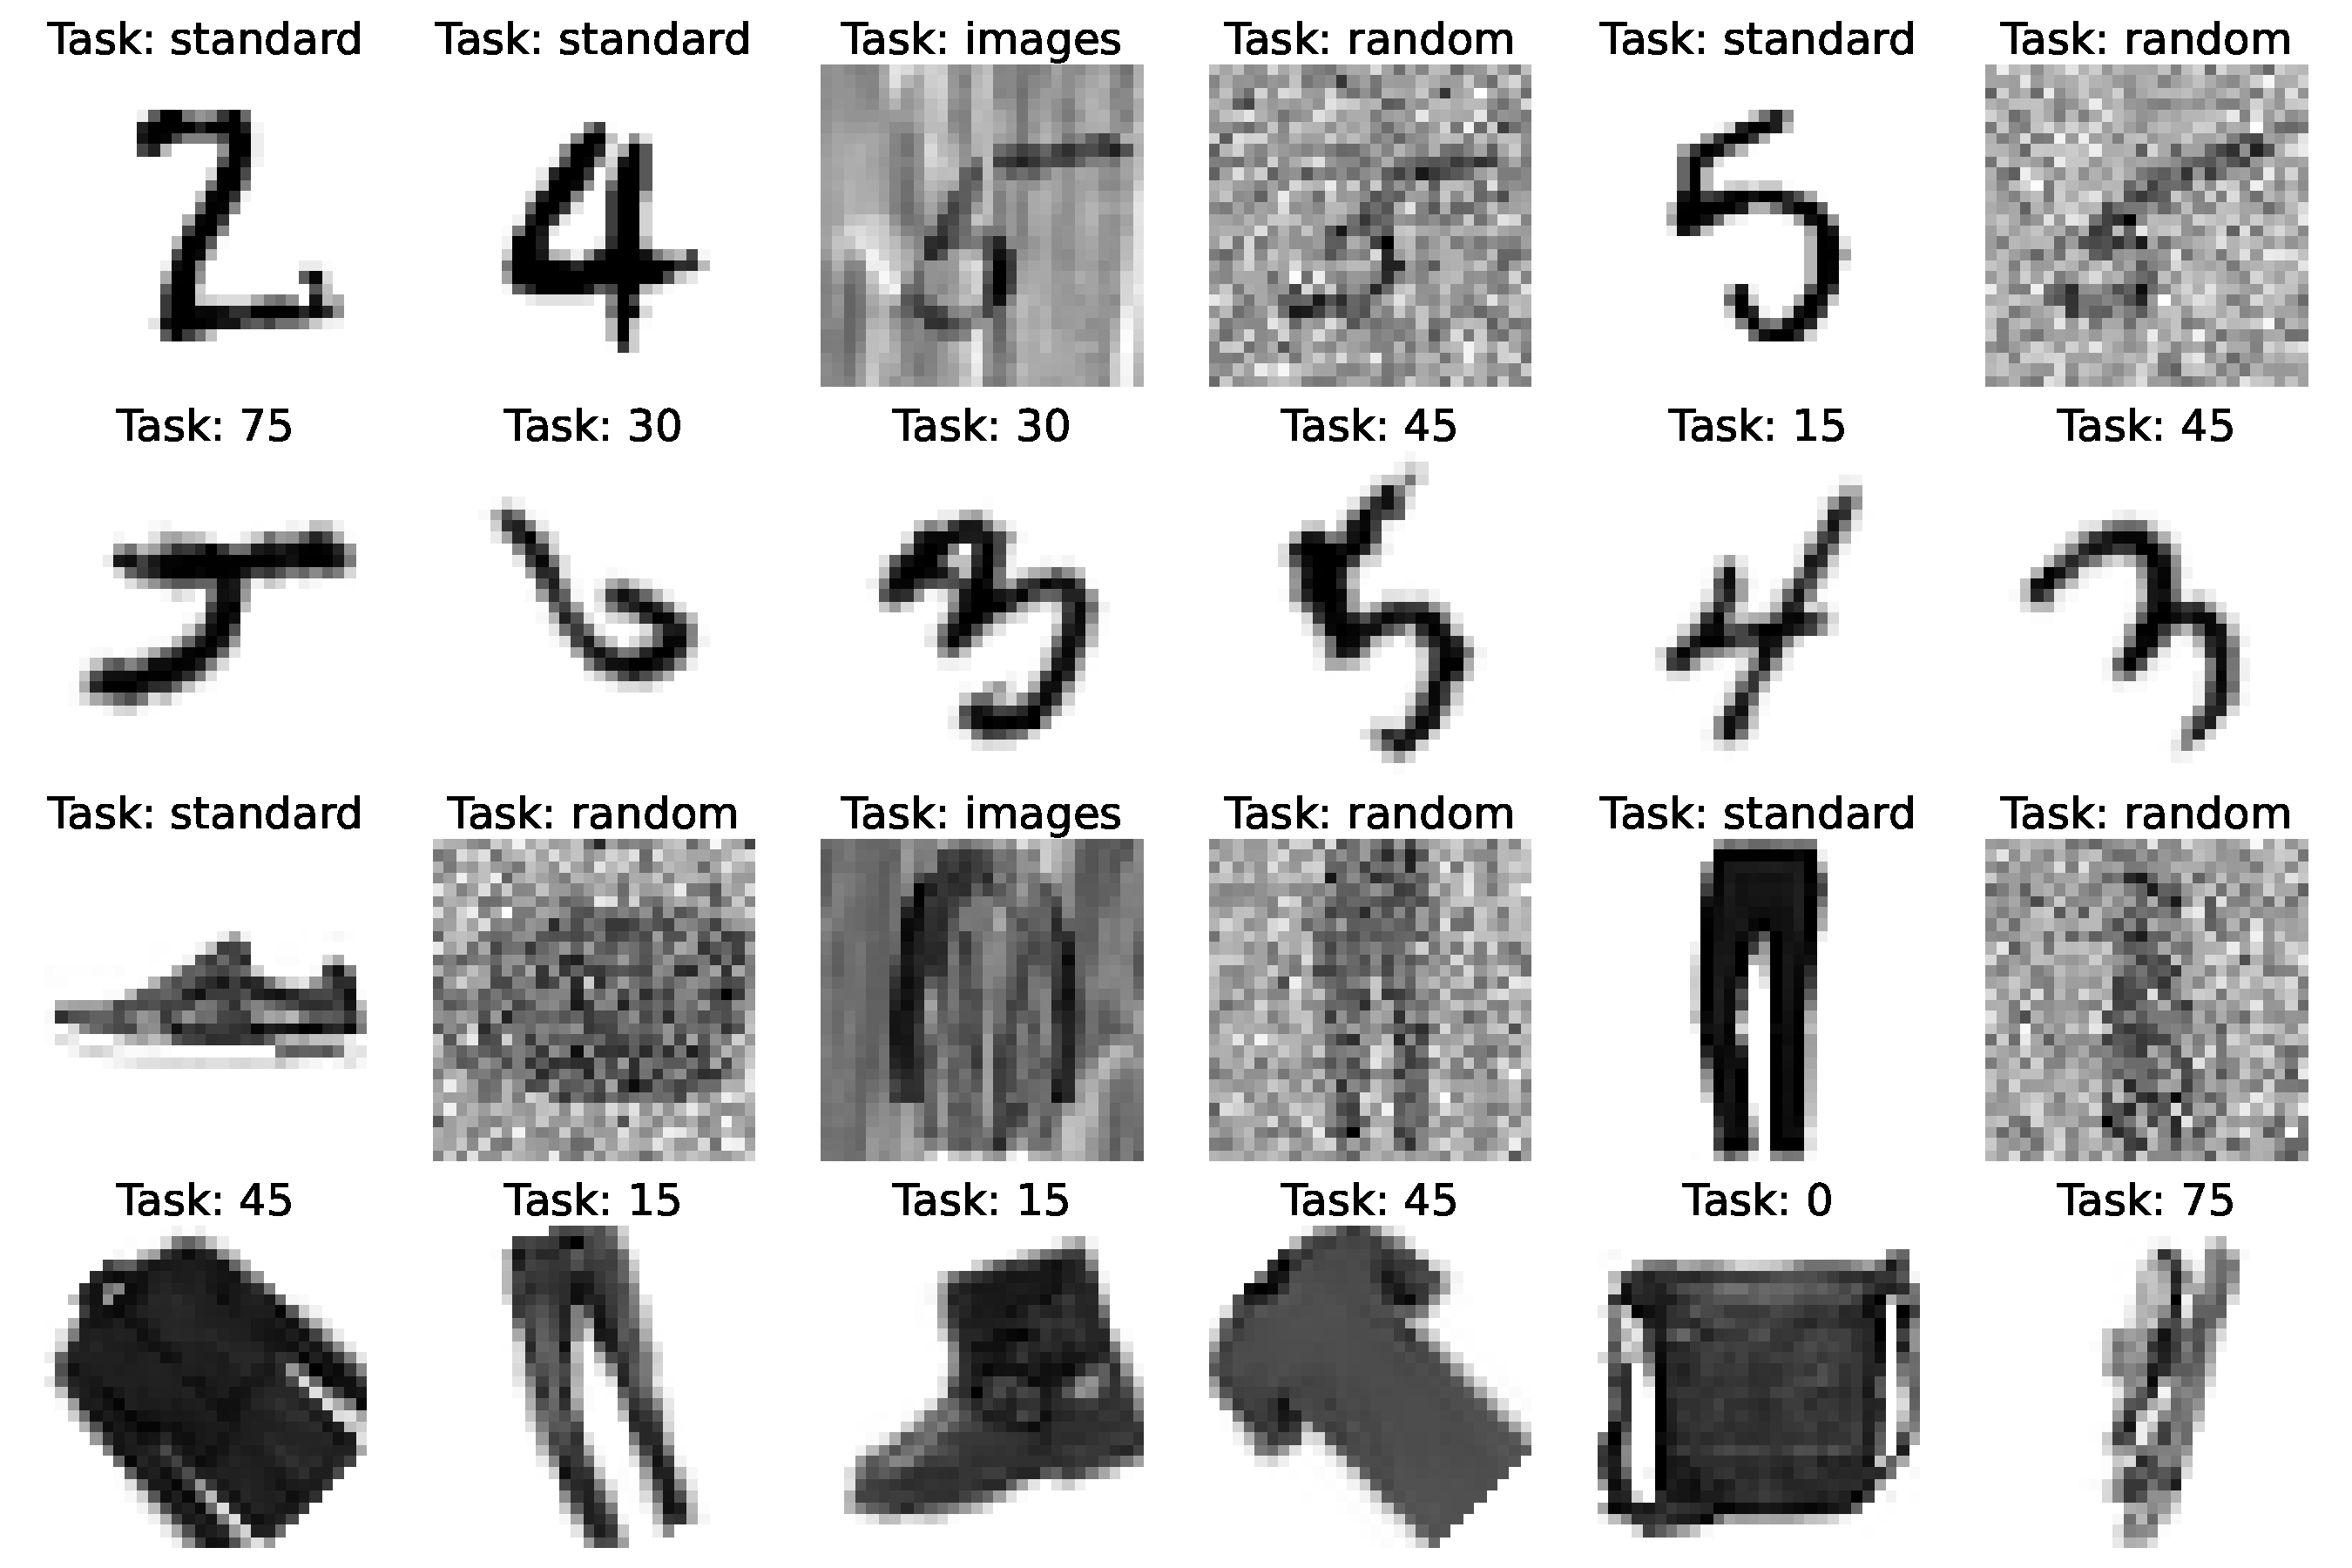
\includegraphics[width=\linewidth]{Chapter4/HAIS2022/hais22_datasets.pdf}
    \caption{Images of the four classification problems used. Each image has a title indicating the corresponding task. The rows correspond to \fdata{var-MNIST}, \fdata{rot-MNIST}, \fdata{var-FMNIST} and \fdata{rot-FMNIST} (from top to bottom).}
    \label{fig:problems_hais2022}
\end{figure}

\paragraph*{Problems Description.\\}
To test the Convex MTL neural networks we use four Multi-Task image datasets:
\fdata{var-MNIST}, \fdata{rot-MNIST}, based on MNIST~\citep{LeCunBBH98}, and \fdata{var-FMNIST}, \fdata{rot-FMNIST}, based on fashion-MNIST~\citep{xiao2017}.
%
The MNIST and fashion-MNIST datasets are both composed of \num{70000} examples of $28\times 28$ grey-scale images. The MNIST dataset contains images of handwritten numbers, while the fashion-MNIST has images of clothes and fashion-related objects.
Both are used as classification problems, where the images have to be classified in one of $10$ possible classes. These classes are balanced in both datasets.
%
To generate the Multi-Task image datasets that we use, we take the images from MNIST or fashion-MNIST and use either the \emph{variations} procedure or the \emph{rotation} one.

%
For the \fdata{var-MNIST} and \fdata{var-FMNIST} we use the \emph{variations} procedure. Inspired by the work of~\cite{BergstraB12}, we consider three transformations:
\begin{itemize}
    \item \textit{random}: adding random noise to the original image.
    \item \textit{image}: adding a random patch of another image to the original image.
    \item \textit{standard}: no transformations are applied to the original image.
\end{itemize}
Then, we use a random split to divide the original datasets in three groups. Each group is applied one of the transformations defined, so we get three tasks: two with \num{23333} examples and the third one with \num{23334}.

%
For the \fdata{rot-MNIST} and \fdata{rot-FMNIST} we use the \emph{rotations} procedure. Using the definitions of~\cite{GhifaryKZB15}, we consider six transformations:
\begin{itemize}
    \item \textit{0}: rotating $0^{\circ}$ the original image.
    \item \textit{15}: rotating $15^{\circ}$ the original image.
    \item \textit{30}: rotating $30^{\circ}$ the original image.
    \item \textit{45}: rotating $45^{\circ}$ the original image.
    \item \textit{60}: rotating $60^{\circ}$ the original image.
    \item \textit{75}: rotating $75^{\circ}$ the original image.
\end{itemize}
Again, we use a random split to divide the original datasets in six groups and each group is applied one of the transformations defined, so we get six tasks: four with \num{11667} examples and two with \num{11666}.
%

In Figure~\ref{fig:problems_hais2022} we show examples of the four MTL image problems that we generate, with the corresponding task annotation for each one.



\paragraph*{Experimental Procedure.\\}
% Models Considered
For testing the performance of our proposal we consider the following models:
\begin{itemize}
    \item \fmod{ctlNN}: a CTL-based neural network, that is, a single network for all tasks.
    \item \fmod{itlNN}: an ITL-based neural network, that is, an independent network for each task.
    \item \fmod{hsNN}: a MTL-based neural network using the hard sharing strategy. That is, a single neural network is used for all tasks, where the first layers are shared among tasks, but a task-specific output layer is used for each task.
    \item \fmod{cvxmtlNN}: a MTL-based neural network using the convex formulation we propose.
\end{itemize}
% convNet
All of these models are based on convolutional network, which we will name \fmod{convNet}, whose architecture is based on the Spatial Transformer Network~\citep{Jaderberg_2015} used in Pytorch\footnote{\href{www.pytorch.org/tutorials/intermediate/spatial\_transformer\_tutorial.html}{www.pytorch.org/tutorials/intermediate/spatial\_transformer\_tutorial.html}}.
The architecture of \fmod{convNet} consists, in this order, on two convolutional layers of kernel size $5$, with $10$ and $20$ output channels each; then a dropout layer, followed by a max pooling layer, and two hidden layers with $320$ and $50$ neurons. After this, the output layers follow.

%
In the \fmod{ctlNN}, we use a single network with the \fmod{convNet} architecture with $10$ output neurons, one for each class.
%
In the \fmod{itlNN}, an independent network, with the \fmod{convNet} architecture and $10$ output neurons, is used for each task.
%
For the \fmod{hsNN}, a single network with the \fmod{convNet} architecture is used, but we have a group of $10$ output neurons for each task in the problem. For example, if we are using of the \emph{rotation}-based problems, we would have $60$ output neurons, but only the group of $10$ corresponding to each task is used with each example.
%
In the \fmod{cvxmtlNN} we use a network with the \fmod{convNet} architecture and $10$ output neurons to model the common network and each of the task-specific networks. That is, given an example from task $r$, the $10$ common output neurons and the  $r$-th task-specific ones are combined to obtain the final output. 

% Optimizer and Hyperparameters
We use the AdamW algorithm~\citep{LoshchilovH19} to train all the models considered, and the weight decay parameter $\mu$ for each model is selected using a CV-based search over the values $\set{10^{-4}, 10^{-3}, 10^{-2}, 10^{-1}, 10^{0}}$. The rest of the parameters, which are part of the architecture, are fixed and set to the default values: the dropout rate is $0.5$ and we use a $2\times 2$ max pooling layer with a stride of $2$.
%
The \fmod{cvxmtlNN} model also has $\lambda$ as a hyperparameter, and it is selected, alongside $\mu$, using a CV grid search, where the grid for $\lambda$ is $\set{0, 0.2, 0.4, 0.6, 0.8, 1}$.

%
The train and test sets are generates using a task-stratified split of $70\%$ and $30\%$, respectively.
The CV grid searches are carried out using the training set, where we use a $5$-fold CV scheme. These folds are task-stratified, that is, all have the same task proportions. Also, since the problems are class-balanced and the sample size is reasonably large, the folds are expected to be class-balanceda as well.

\paragraph*{Results.\\}

\begin{table}[t!]
    \centering
        \caption{Test Accuracy with Majority Voting.}
        \label{tab:test_accuracy_majority}
    \begin{tabular}{l*{4}{c}}
        \hline
                           &   \fdata{var-MNIST} &   \fdata{rot-MNIST} &   \fdata{var-FMNIST} &   \fdata{rot-FMNIST} \\
        \hline
         \fmod{ctlNN} &              0.964 &           0.973 &                     0.784 &                  0.834 \\
         \fmod{itlNN} &              0.968 &           0.981 &                     0.795 &                  0.873 \\
         \fmod{hsNN}  &              0.971 &           0.980  &                    0.770  &                 0.852 \\
         \multirow{2}*{\fmod{cvxmtlNN}} &              \fmaxn{0.974} &           \fmaxn{0.984} &                     \fmaxn{0.812} &                  \fmaxn{0.880} \\
         & ($\lambda^* = {0.6}$)  & ($\lambda^* = {0.8}$) & ($\lambda^* = {0.6}$)  & ($\lambda^* = {0.6}$) \\
         \hline
        \end{tabular}
        
\end{table}

\begin{table}[t!]
    \centering
        \caption{Test Mean Categorical Cross Entropy.}
        \label{tab:test_crossentropy_mean}
    \begin{tabular}{l*{4}{c}}
        \hline
                           & \fdata{var-MNIST}   & \fdata{rot-MNIST}     & \fdata{var-FMNIST}   & \fdata{rot-FMNIST}   \\
        \hline
         \fmod{ctlNN} & 1.274 $\pm$ 0.143  & 1.145 $\pm$ 0.039 & 2.369 $\pm$ 0.183         & 1.757 $\pm$ 0.075      \\
         \fmod{itlNN} & 1.072 $\pm$ 0.029  & 0.873 $\pm$ 0.058 & 2.356 $\pm$ 0.130         & 1.598 $\pm$ 0.042      \\
         \fmod{hsNN}  & 1.087 $\pm$ 0.253  & 0.898 $\pm$ 0.073 & 3.067 $\pm$ 0.888         & 1.888 $\pm$ 0.075      \\
         \multirow{2}*{\fmod{cvxmtlNN}} & \fmaxn{0.924} $\pm$ \fmaxn{0.024}  & \fmaxn{0.831} $\pm$ \fmaxn{0.029} & \fmaxn{2.147} $\pm$ \fmaxn{0.090}         & \fmaxn{1.482} $\pm$ \fmaxn{0.063}      \\
         & ($\lambda^* = {0.6}$)  & ($\lambda^* = {0.8}$) & ($\lambda^* = {0.6}$)  & ($\lambda^* = {0.6}$)      \\
         \hline
        \end{tabular}
\end{table}

% Refitting models
To get more accurate results, less sensitive to randomness, we train each model $5$ different times. To do this, once the optimal hyperparameters have been selected using the CV in the training set, we refit the model with these hyperparameters using the whole training set. That is, the CV is done only once for each model in each problem, but then we repeat $5$ times the procedure of training the network over the whole training set.

% Accuracy vs Categorical CE
Although maximizing the accuracy is ultimately the goal in classification problems, it is not a differentiable measure, so we use the categorical cross entropy instead as the loss function to train the networks. Both measures are correlated, but they do not represent exactly the same behavior. We will show the results using both for completeness.

% Tables
Since we have $5$ instances of each model, a typical strategy to combine their predictions is majority voting. We perform this majority voting directly using the logits, in the output neurons, of each instance and averaging them, so we have $10$ values, one for each class.
In Table~\ref{tab:test_accuracy_majority} we show the test accuracy, using the logits average already described, for each of the approaches considered.
%
Other approach to visualize these results is to compute the categorical cross entropy directly on the averaged logits, which we show in Table~\ref{tab:test_crossentropy_mean}.
%
In both tables we also show the optimal values for $\lambda$ selected in the CV.

% Analysis
Our proposal, the \fmod{cvxmtlNN} model, obtains the best results in all the problems, either in terms of accuracy or cross entropy.
The ITL approach comes second in all problems, except for the accuracy score in \fdata{var-MNIST}, where the \fdata{hsNN} is second and \fdata{itlNN} goes third.
The \fdata{hsNN} model goes third in the rest of problems, while the \fdata{ctlNN} gets the worst results consistently in all problems, sometimes by a large margin.
%
By looking at the tables, it seems that a CTL approach is not able to capture the different properties of each task at once. On the other hand, the \fmod{ITL} approach obtains good results, because it is specialized in each task.
Considering the optimal values for $\lambda$, there are, however, common information shared among the tasks. These values fall far from the margins, so neither the CTL nor the ITL are optimal approaches. This is reflected in the tables, where the \fmod{cvxMTLNN} outperforms consistently \fmod{ctlNN} and \fmod{itlNN}. We can assume, then, that the information learned by the common network and the task-specific ones is complementary, because their combination lead to better results.
%
The hard sharing approach, although better than a CTL one, seems to be too rigid to effectively capture the differences among different tasks, so it is frequently surpassed by the ITL network.




% Complementing common and task-specific



\section{Application to Renewable Energy Prediction}\label{sec:convexmlt_renewable}

A transition towards renewable energies is taking place, with particular interest for solar and wind generation, which implies a demand for accurate energy production forecasts to be made for the transmission system operators, wind and solar farm managers and market agents. These forecasts can be made at different time horizons: very short (up to one hour), short (up to a few hours), or medium-long (one or more days ahead).
In this application of our convex MTL techniques to renewable energies forecast, we will focus wit the latter, in particular, the hourly, day-ahead prediction, that is, the prediction of tomorrow, at each hour, is predicted today.

Machine Learning (\acrshort{ml}), like in others forecasting problems, have an increasing presence in the energy prediction approaches. 
The usage of ML models require choosing the predictive features that will be used, which depends on the time horizon of interest. 
For short-term forecast, past values of energy production and real time meteorological data can be used; however, for longer horizons, the most common features are numerical weather predictions (\acrshort{nwp}), that can be provided by entities such as the \acrlong{ecmwf}, which is the one used in this work.
For the hourly day-ahead predictions of interest here, we use the NWP forecasts of the ECMWF run at \utc{00} in a given day to predict the hourly energy productions the day before. That is, using the NWP of \utc{00}, the energy generation predictions are given for each hour from {24} to {47}h.

After the selection of predictive features, the ML method better suited for the problem at hand has to be selected. Also, each method has a set of hyperparameters that influence on its behaviour and have to be adjusted in each case.
In the case of interest here, there are two possibilities: using local models for single installations or global models for multiple installations within a geographic area.

% Many ML approaches have been proposed for energy forecasting. 
% In the case of wind energy, prediction see, for example, the reviews of wind energy predictions of~\citep{giebel_soa,pinson2013,colak} or the application of concrete models to specific time-horizons~\citet{heinermann,zhu_genton}.
% For solar energy, we can see the surveys of~\citep{Antonanzas2016,Inman2013,Wan2015}, and a good reference for many aspects of photovoltaic energy can be found in~\cite{SEK}.

Anyway, any ML approach has to deal with the changing behaviour of a wind or solar farm, which can be altered substantially according to different conditions or time.
In the PV energy production this is obvious, since different times of the day, from sunrise to sunset, have very different behaviours; but there are also seasonal effects that affect the energy generation in the solar farms.
For wind energy, it is more difficult to define the variables that determine different scenarios. 
The energy velocity forecast is the most relevant variable for energy generation, but it is important to take into account the power curve of wind turbines, which has three different response zones: one for low speed and near zero production, an intermediate one with power growing with wind velocity and one with~maximum constant power up to the cut-off speed.
The angle in which this wind incide is also important, since the turbines of a farm have a specific direction. 
Finally, the assymetrical wind velocities between the day and night period can also affect the energy production.

One way to deal with this different behaviour scenarios is to apply a MTL model, where the models built are specialized in each scenario but all scenarios are used in the learning process.
In this Section a convex MTL approach will be used for wind and solar energy forecasting. To do this, it is necessary to define the tasks of interest on each case, which are described in the following subsections.
In the first subsection the experimental methodology is described, showing how the models are chosen and the hyperparameters are selected. Then, the next two subsection presents the approach and the detailed task definitions used for solar and wind energy, respectively, as well as the results to judge the resultant performance.

\subsection{Experimental~Methodology.\\}

%
\begin{table}[t!]
    \caption{Hyperparameters, grids used to find them (when appropriate), and hyperparameter selection method for each model. Here, $d$ is the number of {dimensions} % Please chang the font in the Table.
     of the data and $\sigma$ is the standard deviation of the~target.}
    \label{tab:hyperpars_grid_energies}
    \centering
     \begin{tabular}{*{5}{c}}
     \toprule
     \fhead{Par.} & \fhead{Grid} & \fhead{ctlSVR} & \fhead{itlSVR} & \fhead{cvxMTL} \\
     \midrule
      $C$ &  $\set{10^k: -1 \leq k \leq 6}$ & CV & CV & CV  \\
      $\epsilon$ & $\set{\frac{\sigma}{2^k}: 1 \leq k \leq 6}$ & CV & CV & CV  \\
      $\gamma$ & $\set{\frac{4^k}{d}: -2 \leq k \leq 3}$ & CV & - & ctlSVR \\
      $\gamma_r$ & $\set{\frac{4^k}{d}: -2 \leq k \leq 3}$ & - & CV & itlSVR\\
      $\lambda$ & $\set{10^{-1}k: 0 \leq k \leq 10}$ & - & - & CV \\
      \bottomrule
     \end{tabular}
\end{table}

Here we describe the methodology that we have followed to conduct the experiments of renewable energy prediction.
%
For the solar and wind energy we use the same procedure. In each problem, we have a train, validation and test sets, each corresponding to one year of data. In the solar energy problems we have 2013, 2014 and 2015 as train, validation and test sets, respectively; while for wind energy problems we use 2016, 2017 and 2018.
%
For both solar and wind problems we use different definition of tasks. To define these tasks we use only the training data, which partition the data, then, with these tasks' definition, we apply them to get the tasks of the validation and test examples.
%
For example, if we use the wind velocity to define three tasks, we study the velocities of the training examples to set the boundaries that define each task; then, we use this definitions on the validation and test sets.
%
We will represent the task definition applied with the nomenclature: \fmodt{taskDef}{modelName}, where \fmod{taskDef} is a name for the task definition and \fmod{modelName} is the name of the model.

%
We consider three different models based on the standard Gaussian kernel SVR:
\begin{itemize}
    \item \fmod{ctlSVR}: a CTL model, that is, a single SVR for all tasks. Its set of hyperparameters is $\set{C, \gamma, \epsilon}$, where $C$ is the regularization trade-off parameter, $\gamma$ is the kernel width, and $\epsilon$ the width of the error insensitive area.
    \item \fmod{itlSVR}: an ITL model, that is, an independent SVR for each task. For each task, we have standard SVR with its hyperparameters: $\set{C_r, \gamma_r, \epsilon_r}$ for $r=1, \ldots, \ntasks$.
    \item \fmod{mtlSVR}: a convex MTL model, as shown in Subsection~\ref{subsec:cvx_l1-svm}, with its corresponding set of hyperparameters is $\set{C, \epsilon, \gamma, \gamma_1, \ldots, \gamma_\ntasks, \lambda_1, \ldots, \lambda_\ntasks}$, where $\gamma$ is the kernel width of the common part and $\gamma_r$ the one of the $r$-th specific part; also, $\lambda_r$ is the convex combination parameter corresponding to the $r$-th task.
\end{itemize}
%
Although the CTL approach does not use the tasks information, the ITL and MTL models depend on the task definition that we use. For example, prediction at different hours can define different tasks, where the possible values are, for example, (\fmod{hour}=14) or (\fmod{hour}=12). The models using this task definition will be named \fmodt{hour}{itlSVR} and \fmodt{hour}{mtlSVR}. 
%
Since each task definition partition the data, we can also use multiple task definitions, combining them and creating finer partitions. 
We will name \fmod{(taskDef1,...,taskDefM)} the combination of task definitions \fmod{taskDef1}, ..., \fmod{taskDefM}. For example, consider the \fmod{(hour)} definition, which, in our definition consider 14 different hours, hence, 14 tasks; and consider the \fmod{season} definition, which considers the prediction in each season as a different task, hence, four tasks. The combined definition \fmod{(hour, season)} generates $14 \times 4$ possible tasks, whose values can be, for example, \fmod{(hour = 12, season = summer)}.
The models using this combination will be named \fmodt{hour, season}{itlSVR} or \fmodt{hour, season}{mtlSVR}.

%
As explained in Subsection~\ref{subsec:cvx_l1-svm}, the cost of methods to select the optimal hyperparameters scale exponentially with the dimension, so it is not feasible to use a CV grid search, for example, if we have more than $3$ hyperparameters.
%
In the \fmod{ctlSVR} and \fmod{itlSVR} it is not a problem, since we have $3$ hyperparameters, for the common, single SVR, and for the task-independent ones, respectively. We use then a CV grid search, using as train and validation sets described above.
However, to find the hyperparameters of \fmod{mtlSVR} we have to make some adjustements, as shown in Subsection~\ref{subsec:convexmtlsvm_exp}. 
%
First, we use a convex MTL formulation with a single $\lambda$ parameter, common to all tasks.
%
Second, we use the optimal kernel widths selected in validation for the CTL and ITL approaches as the widths in the MTL approach. That is, we get the optimal common $\gamma^*$ and task-specific $\gamma^*_1, \ldots, \gamma^*_\ntasks$, and fix them in the \fmod{mtlSVR} model, not including them in the grid search procedure.
Then, we use a CV grid search to find the optimal values of the remaining hyperparameters, that is, $\set{C, \epsilon, \lambda}$.
%
In Table~\ref{tab:hyperpars_grid_energies} we show the method to obtain each hyperparameter, as well as the grids used in the CV grid search procedures.
We use the \acrshort{mae} as the validation metric, because is the most natural to the $\epsilon$-insensitive loss that is used in the SVRs.

%
The whole procedure to get the final scores is:
\begin{enumerate}
    \item \textbf{Scaling the target and normalizing the features.} We scale the target values to $[0, 1]$ and we normalize each feature, so it has $0$ mean and a standard deviation of $1$. This is done using the training data only. 
    For the target scale, we select the target minimum and maximum values of the training set, that is, $y_\text{min} = 0$, when no energy is produced, and $y_\text{max}$ is the maximum capacity of the park.    
    %Then, the target in train, validation and test sets is normalized as     $y_\text{scaled} = (y - y^\text{tr}_\text{min}) / (y^\text{tr}_\text{max} - y^\text{tr}_\text{min} )$.
    %For example, for feature normalization, we compute the training mean $\mu_d^\text{tr}$ and standard deviation $\sigma_d^\text{tr}$ of feature $d$, then we normalize the corresponding feature in the whole dataset using $\hat{X}_d = (\hat{X}_d - \mu_d^\text{tr}) /  \sigma_d^\text{tr}$.
    \item \textbf{Using a CV grid search to select the optimal hyperparameters.} This is done using the train and validation sets, with the grids and adjustements already explained. We use the MAE as our validation metric.
    \item \textbf{Predict on the test set and rescale to the original scale.} That is, we use the corresponding model $f(\cdot)$ to compute the prediction of the normalized $i$-th test example from task $r$, $\tilde{x}_i^r$, as $f(\tilde{x}_i^r)$. Then, we rescale it back to obtain the final prediction $\hat{y}_i^r = f(x_i^r) \times (y_\text{max} - y_\text{min} ) + y_\text{min}$
    \item \textbf{Compute the test score.} Using the target values $y_i^r$ and their corresponding predictions, $\hat{y}_i^r$, we measure the performance of our model using both MAE and MSE.
\end{enumerate}
The whole process is carried out using a \fcode{Pipeline} object, where we make use of class \fcode{StandardScaler} to normalize the data, and \fcode{TransformedTargetRegressor} class to scale the targets. All these classes are part of the \emph{scikit-learn} library.

%
To put our results in perspective, we also show the errors of simple persistence models and of multilayer perceptrons. For the perceptron we use the \fcode{MLPRegressor} class of \emph{scikit-learn}. The architecture for both problems consists on fully connected networks with two hidden layers, with $100$ and $50$ neurons. We train these networks using the L-BFGS solver with a maximum of $800$ iterations a tolerance of $10^{-10}$. The regularization hyperparameter is selected using a CV grid search, as those described above, where the grid is $\set{4^k: -2 \leq j \leq 3}$.






\subsection{Solar Energy}
The goal is to predict the hourly energy production in two parks, located in the islands of Majorca and Tenerife, and name the corresponding problems as \fdata{majorca} and \fdata{tenerife}, respectively. 
%
In this subsection the experiments with these solar problems are presented, using the experimental procedure already shown. First a description of the problems is given and the data used, then the results are given and analyzed.

\paragraph*{Data and~Tasks.\\}
For both problems, \fdata{majorca} and \fdata{tenerife}, the same variables, extracted from the Numerical Weather Prediction (NWP), are used. These variables, extracted from NWP predictions made by the European Center for Medium Weather Forecasts 
(ECMWF;~\cite{ECMWF}), are:
\begin{itemize}
    \item Surface net solar {radiation} (\ftt{SSR}).
    \item Surface solar radiation {downwards} (\ftt{SSRD}).
    \item {Total Cloud Cover} %Please change it not to be captitalized if unnecessary.
     (\ftt{TCC}).
    \item Temperature at 2 {meters} (\ftt{T2M}).
    \item Module of the speed of wind at {10 meters} (\ftt{v10}).
\end{itemize}
The radiation variables \ftt{SSR}, solar radiation, and \ftt{SSRD}, solar radiation plus the diffuse radiation scattered by the atmosphere, as well as the \ftt{TCC}, have all a direct impact on PV production.
%
The \ftt{T2M} and \ftt{v10} features are also considered because they influence the conversion of photon energy into electrical one, and also the overall performance of PV stations.
%

To collect these features, geographical grids with a $\ang{0.125}$ spatial resolution are considered. For \fdata{majorca}, the grid has its northeast coordinates at $(\ang{2}, \ang{40})$, and its southwest coordinates at $(\ang{4}, \ang{39})$. For \fdata{tenerife}, the coordinates are $(\ang{-17.5}, \ang{28.75})$ for the northeast corner, and $(\ang{-15.5}, \ang{27.75})$ for the southwest one.
%
That is, both grids have a longitude width of 2 degrees and a latitude height of 1 degree. With the spatial resolution considered, this results in a total number of $17 \times 9 = 153$ grid points; since we use five variables at every point, the total dimension of our data is thus $5 \times 153 = 765$. 


%
Observe that we obtain large dimensional patterns, where the features might be highly correlated. That is, a feature, \ftt{SSR} for example, measured in one point of the grid and another close point might be very correlated, since the grids are squares with sides of about $\km{12}$.
This correlation will affect those models based on matrix-vector computations, such as linear models, which are the most obvious, but, also, to some extent, to neural networks.
Although Ridge or Tikhonov regularization can alleviate this issue for these models, the kernel-methods, such as the kernel SVMs, seems better suited for these kind of problems.
When we use kernel methods, such as the Gaussian kernel $\exp{-\gamma \norm{x-y}^2}$, the algorithm learns using the distances among patterns $\norm{x - y}$, instead of its features.
%
These distances scale linearly with the dimension of data, that is, consider the features scaled to $[0, 1]$, then a rough estimate of the distance between two patterns would be $d$. In the extreme case where all features are equal, i.e. $x_j = x_1$ for all $j=1, \ldots, \dimx$; then, $\norm{x - x'} = d(x_1 - {x'}_1)$.
However, this influence of the dimension can be easily controlled by $\gamma$, and, if selected properly, should not affect the performance of a Gaussian SVR.

%
Recall that we use data from years 2013, 2014 and 2015 as train, validation and test sets, respectively.
%
We show the errors in both total \mwhu{} and as percentages, in the range $[0, 100]$ of the total install PV power in each photovoltaic park, {\mw{72.46}} in \fdata{majorca} and \mw{107.68} in \fdata{tenerife}.
%
We remove night data for obvious reasons and make predictions between \utc{06} and \utc{19} {for} \fcode{majorca} and between \utc{07} and \utc{20} for \fcode{tenerife}.
%
The hour of the day has a direct influence on the solar radiation, and, therefore, on energy production. Also, the season of the year has a similar impact on the production. This leads to two obvious task definitions:
\begin{itemize}
    \item	\fcode{hour}: The prediction at each hour is defined as a different task; there are thus 14 tasks in \fcode{majorca} (from 06 to \utc{19}) and \fcode{tenerife} (from 07 to \utc{20}).
    %We observe in Figures~\ref{fig:maj_groupby_hour} and~\ref{fig:ten_groupby_hour} that the distribution of the target, i.e.,~the photovoltaic energy, is very dependent on the hour chosen.
    \item	\fcode{season}: The prediction at each season is defined as different task.  With~a slight abuse of language, the definitions for each season used are: Spring, from~16 February to 15 May; Summer, from~16 May to 15 August; Autumn, from~16~August to 15 November; and~Winter, from~16 November to 15 February.
    %We can observe in Figures~\ref{fig:maj_groupby_season} and~\ref{fig:ten_groupby_season} that different seasons have different means of the target.
\end{itemize}
%
In Subfigures~\ref{fig:maj_groupby_hour} and~\ref{fig:ten_groupby_hour} the hourly averages of the PV energy in \mwhu{} are shown for \fdata{majorca} and \fdata{tenerife}.
Also, in Subfigures~\ref{fig:maj_groupby_season} and~\ref{fig:ten_groupby_season} the monthly averages, colored by season.
\begin{figure}[H]
    \centering%
    \subfloat[][]{%    
    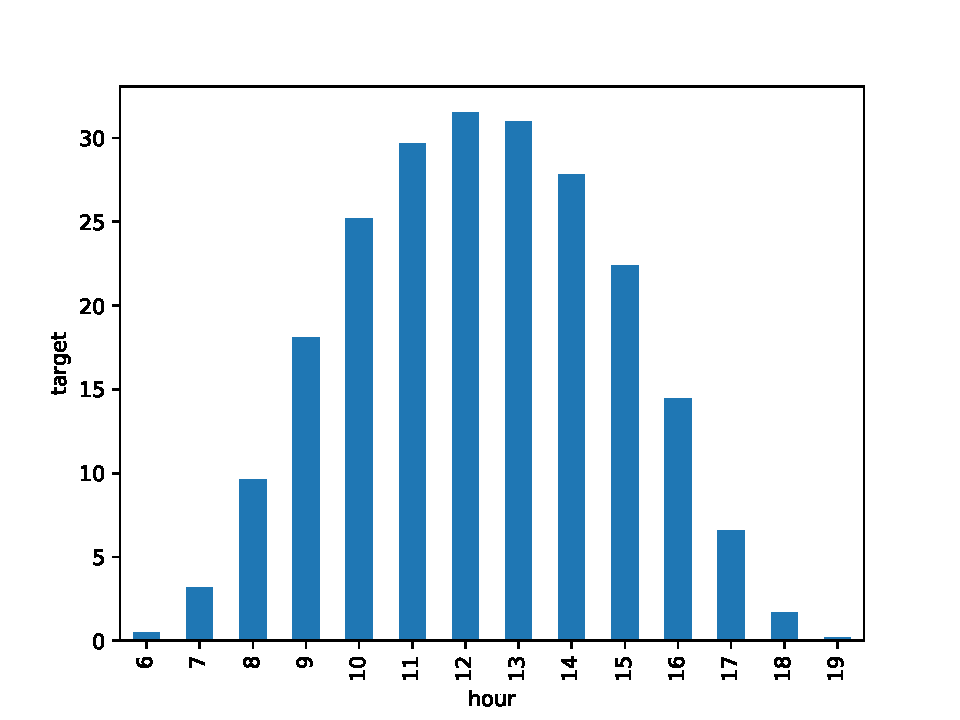
\includegraphics[width=.35 \textwidth]{Chapter4/energies/majorca_groupby_hour_train.pdf}
    \label{fig:maj_groupby_hour}}\quad%
    \subfloat[][]{%
    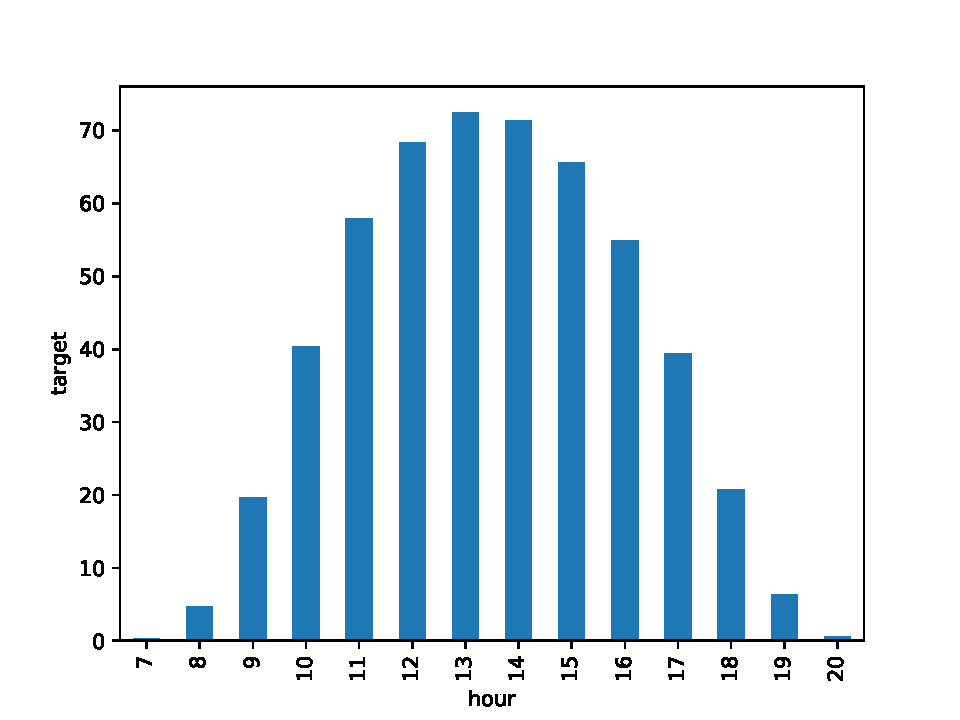
\includegraphics[width=.35 \textwidth]{Chapter4/energies/tenerife_groupby_hour_train.pdf}
    \label{fig:ten_groupby_hour}}\\
    \subfloat[][]{%
    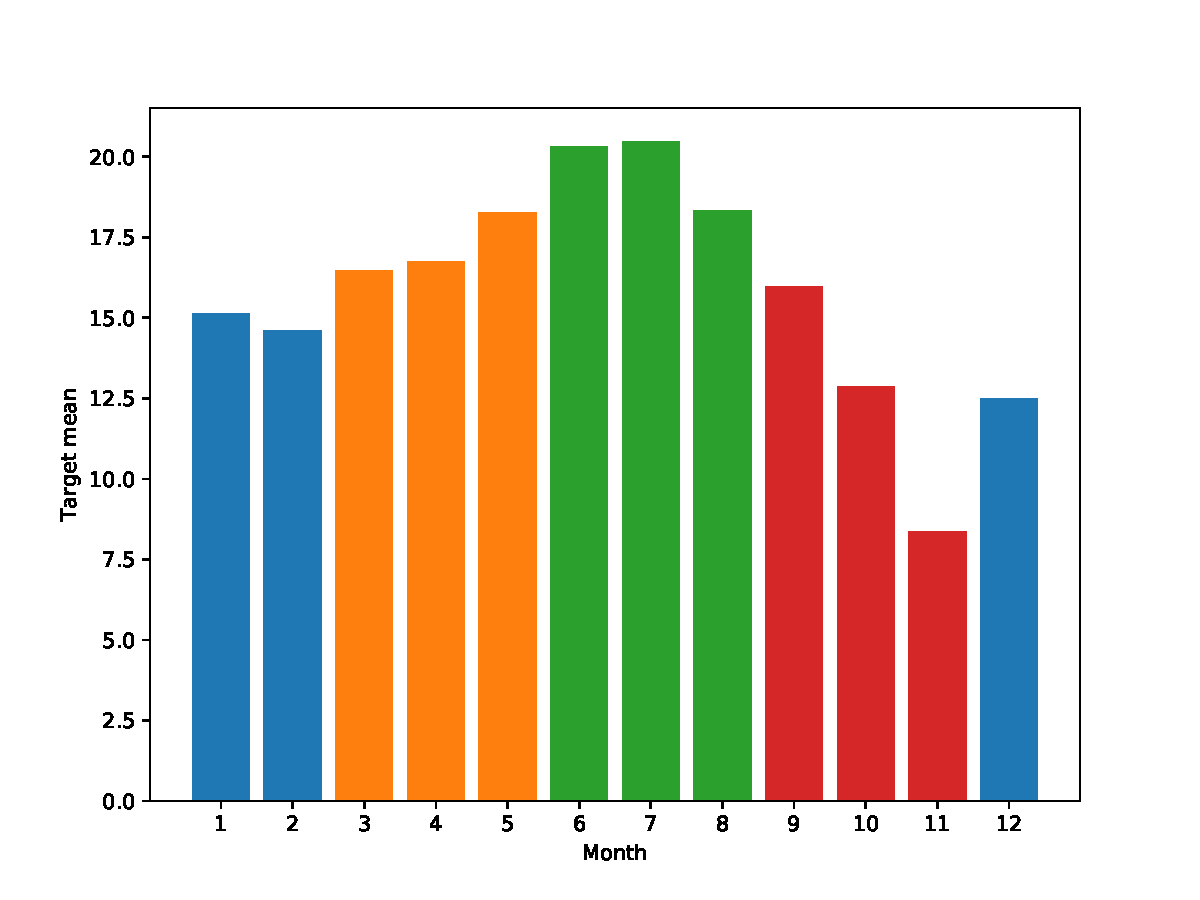
\includegraphics[width=.35 \textwidth]{Chapter4/energies/hist_season_majorca_train_byMonth.pdf}
    \label{fig:maj_groupby_season}}\quad%
    \subfloat[][]{%
    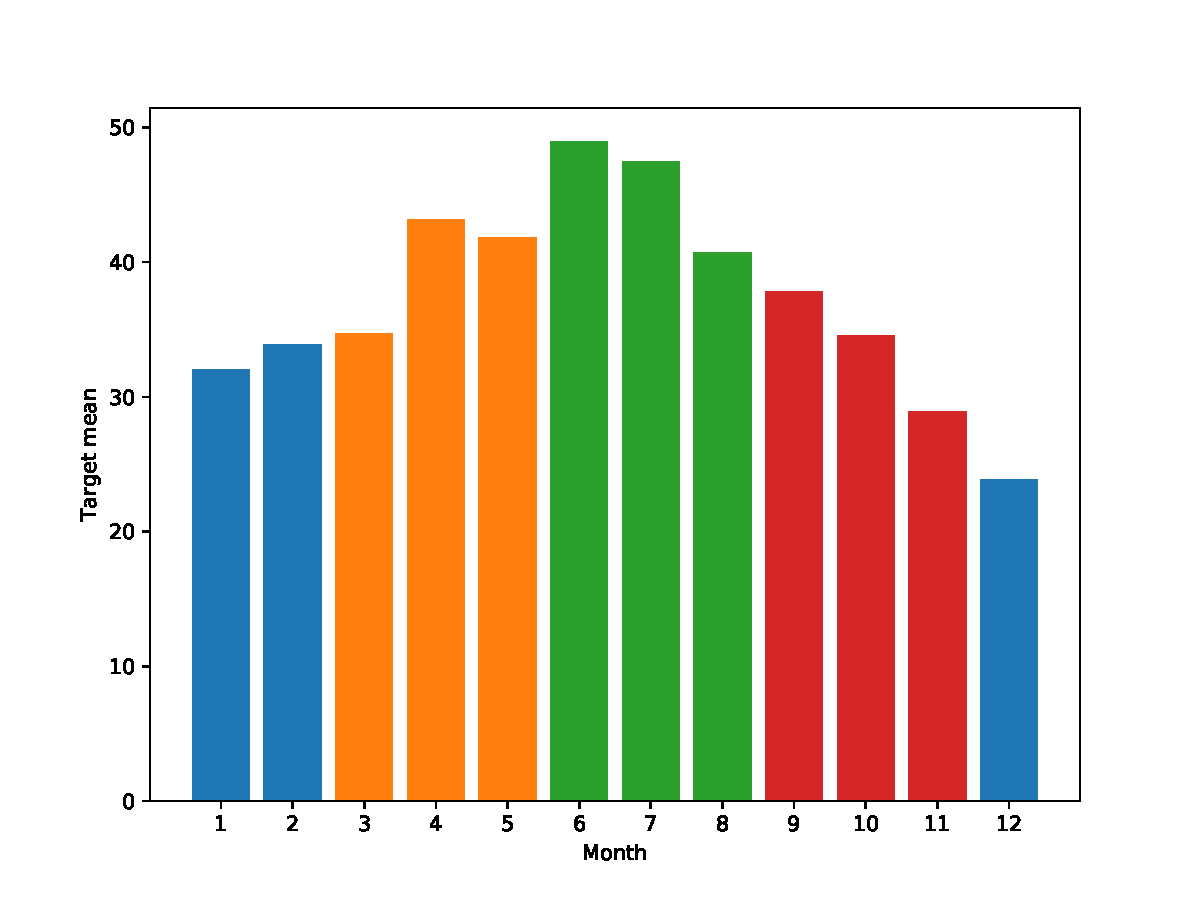
\includegraphics[width=.35 \textwidth]{Chapter4/energies/hist_season_tenerife_train_byMonth.pdf}
    \label{fig:ten_groupby_season}}
 \caption{\label{fig:solar_task_def}Hourly photovoltaic energy mean {in} \fcode{majorca}~\protect\subref{fig:maj_groupby_hour} {and}~\fcode{tenerife}~\protect\subref{fig:ten_groupby_hour} measured in \mwhu{}. Photovoltaic energy monthly averages for \fcode{majorca}~\protect\subref{fig:maj_groupby_season} and \fcode{tenerife}~\protect\subref{fig:ten_groupby_season} , colored using the tasks defined using the season and measured in \mwhu{}. All the histograms have been computed using data from year~2016.}
 \end{figure}
 




\paragraph*{Experimental~Results.\\}

\begin{table}[H]
    \caption{Test MAEs (left), test MSEs (center), and optimal mixing $\lambda^*$ (right) of the solar energy models considered {in} \fcode{majorca}. {Base units} %Is the bold in the Table necessary? If is not necessary, please remove it. Also, please remove the font in the table. Same as below.
     are either \mwhu{} or percentages (\%). The~best model errors are shown in~bold.}
    \centering
    \label{table:solar_scores_m}
 \begin{tabular}{lccccccc}
    \toprule
     & \fheadmulti{3}{MAE} & \fheadmulti{3}{MSE} & \fhead{$\lambda^*$}\\
    & {{\mwhu}}	& {{\%}} & {rank} & {{\mwhu}}	& {{\textpertenthousand}} & {Rank}& \\
    \midrule
    \fmod{ctlSVR}    &  5.265 &  7.265  & (6) &  59.322 &  112.985  & (6) &  - \\
    \fmod{(season)\_itlSVR}   &  5.305 &  7.384  & (7) &  59.591 &  113.498  & (7) &  - \\
    \fmod{(season)\_mtlSVR}   &  \fmaxn{4.884} &  \fmaxn{6.740}  & \fmaxn{(1)} &  53.222 &  101.366  & (2) &  0.4 \\
    \fmod{(hour)\_itlSVR}   &  5.083 &  7.015  & (4) &  54.540 &  103.877  & (3) &  - \\
    \fmod{(hour)\_mtlSVR}   &  4.957 &  6.840  & (2) &  \fmaxn{52.614} &  \fmaxn{100.208}  & \fmaxn{(1)} &  0.3 \\
    \fmod{(hour, season)\_itlSVR}   &  5.250 &  7.251  & (5) &  57.927 &  110.328  & (5) &  - \\
    \fmod{(hour, season)\_mtlSVR}   &  5.038 &  6.952  & (3) &  54.601 &  103.992  & (4) &  0.3 \\
    \bottomrule
    \end{tabular}
 \end{table}
\unskip


 \begin{table}[H]
    \caption{Test MAEs (left), test MSEs (center), and optimal mixing $\lambda^*$ (right) of the solar energy models considered {in} \fcode{tenerife}. Base units are either \mwhu{} or percentages (\%). The~best model errors are shown in~bold. The positions with hyphens correspond to the model ranked first in terms of MAE or MSE, as indicated by its column.}
    \centering
    \label{table:solar_scores_t}
 \begin{tabular}{lccccccc}
    \toprule
     & \fheadmulti{3}{MAE} & \fheadmulti{3}{MSE} & \fhead{$\lambda^*$}\\
    & {{\mwhu}}	& {{\%}} & {Rank} & {{\mwhu}}	& {{\textpertenthousand}} & {Rank}& \\
    \midrule
    \fmod{ctlSVR}    &  5.786 &  5.373  & (5) &   88.323 &  76.174  & (5) &  - \\
    \fmod{(season)\_itlSVR}   &  5.930 &  5.545  & (6) &   97.454 &  84.611  & (6) &  - \\
    \fmod{(season)\_mtlSVR}   &  5.579 &  5.181  & (4) &   86.227 &  74.366  & (3) &  0.8 \\
    \fmod{(hour)\_itlSVR}   &  5.403 &  5.018  & (2) &   86.686 &  74.762  & (4) &  - \\
    \fmod{(hour)\_mtlSVR}   &  \fmaxn{5.376} &  \fmaxn{4.993}  & \fmaxn{(1)} &   \fmaxn{84.207} &  \fmaxn{72.624}  & \fmaxn{(1)} &  0.7 \\
    \fmod{(hour, season)\_itlSVR}   &  6.025 &  5.554  & (7) &  104.536 &  90.297  & (7) &  - \\
    \fmod{(hour, season)\_mtlSVR}   &  5.494 &  5.102  & (3) &   85.440 &  73.687  & (2) &  0.7 \\
    \bottomrule
    \end{tabular}
 \end{table}
\unskip


\begin{table}[H]
   \caption{Wilcoxon $p$-values for absolute (left) and quadratic (right) errors.}
   \centering
   \label{table:solar_wilcoxon}
   %% \tablesize{} %% You can specify the fontsize here, e.g.,~\tablesize{\footnotesize}. If commented out \small will be used. Is the bold necessary. Same as others in the table.
   \begin{tabular}{lcccc}
      \toprule
      & \fheadmulti{2}{MAE} &  \fheadmulti{2}{MSE}\\
      & {\fcode{majorca}}	& {\fcode{tenerife}} & {\fcode{majorca}}	& {\fcode{tenerife}}\\
      \midrule
   \fmod{ctlSVR}                           &    0.014 (4) &    0.000 (5) &    0.081 (4) &    0.000 (5) \\
   \fmod{(season)\_itlSVR}                &    0.008 (5) &    0.636 (5) &    0.215 (4) &    0.354 (5) \\
   \fmod{(season)\_mtlSVR}         &   ------ %MDPI: We changed it into minus, please confirm.
{(1)} &    0.000 (4) &    0.036 (2) &    0.000 (3) \\
   \fmod{(hour)\_itlSVR}                  &    0.693 (2) &    0.006 (2) &    0.000 (3) &    0.000 (4) \\
   \fmod{(hour)\_mtlSVR}           &    0.067 (1) &   ------ {(1)} &   ------ {(1)} &   ------ {(1)} \\
   \fmod{(hour, season)\_itlSVR}        &    0.000 (3) &    0.000 (6) &    0.000 (4) &    0.098 (5) \\
   \fmod{(hour, season)\_mtlSVR} &    0.000 (2) &    0.000 (3) &    0.745 (3) &    0.000 (2) \\
   \bottomrule
\end{tabular}
\end{table}

In Tables~\ref{table:solar_scores_m} and~\ref{table:solar_scores_t} we show the numerical results for \fdata{majorca} and \fdata{tenerife}, respectively. We give the test MAE, which is the most natural metric for SVRs, as well as the MSE. 
In the case of percentages, for MAE, we give the percentage corresponding to the total installed power, and for the MSE, the permyriad, that is per \num{10000}, of the installed power.
%
We also show the rankings in terms of MAE or MSE, and the optimal hyperparameter $\lambda^*$ selected in the CV for the MTL models.
%

To show statistical significance the Wilcoxon test is used, but instead of testing every pair of models, the rankings of Tables~\ref{table:solar_scores_m} and~\ref{table:solar_scores_t} are used. The Wilcoxon test is applied between each model and the next in ranking at the $0.05$ level, to determine if the difference is significant.
The test is applied over the list of errors commited by each model in the patterns of the test set. When the null hypothesis of the Wilcoxon test is refused, it implies that the distribution of the difference between the errors does not have its median at $0$.
In Table~\ref{table:solar_wilcoxon}, we show the $p$-values of the pairwise tests. If the $p$-value is smaller than the level considered level of 0.05, then the different between models is considered significant.
%
With these procedure, a new significant ranking, shown in Table~\ref{table:solar_wilcoxon},  is generated: starting from the best model, we compare each model with the next best one, and we increase the ranking only if the difference is significant.
%
For example, in Table~\ref{table:solar_scores_m}, in terms of MAE, the first model, \fmod{(season)\_mtlSVR}, is tested against the second one, \fmod{(hour)\_mtlSVR}. In Table~\ref{table:solar_wilcoxon}, we show the $p$-value corresponding to that test, which is $0.067$, and since it is larger than the level $0.05$, the ranking is not increased and both models have the same significant ranking. 

%
Looking at the tables, it is easy to see that the MTL approaches obtain the best results in both problems, while \fmod{ctlSVR} has the worst performance in \fcode{tenerife} and second worst in \fcode{majorca}.
ITL models are more difficult to interpret, although they are always behind their corresponding MTL approaches, they can obtain good results, like the \fmodt{hour}{itlSVR} in \fdata{majorca} which is second; but they can also have bad performances, like the \fmodt{season}{itlSVR} in \fdata{tenerife}.

%
The $\lambda^*$ values can help to understand this behaviour. In both problems, the selected values lie far from the extremes $0$ or $1$, which distances the MTL approaches from the CTL or ITL ones. If these values are optimal, then the CTL or ITL equivalent models, with $\lambda=1$ and $\lambda=0$, respectively, obtain a worse result in validation. This is reflected also in the test set, as shown in the tables.
Also, it is noticeable that the optimal values for \fdata{majorca} are all smaller than $0.5$, which can be intepreted as models with a stronger common part, while in \fdata{tenerife}, the optimal values are larger than $0.5$ which reflects stronger independent parts.
%
Although the MTL approaches get the best results with any task definition, the \fmod{(hour)} definition seems to work best than the \fmod{(season)} one. The \fmodt{hour}{mtlSVR} gets a second best result, which is not significantly worse than the best one in \fdata{majorca}, and the single best result in \fdata{tenerife}.

%
For completeness the scores of persistence models and a neural network are given.
The persistence forecasts are obtained by predicting at each hour the target value 24 hours prior. By doing this, the MAE scores for majorca are \mwh{5.776} and \mwh{7.766}, which scaled to $[0, 100]$ correspond to 7.97\% and 7.21\%; which are an 18\% and 44\% error increase of the best MTL models.
The neural network errors are \mwh{5.140} and \mwh{5.763}, that is, 7.09\% and 5.35\% of the total PV installed. While this results are still competitive, this performance is worse than those of the convex MTL models proposed.


\begin{figure}[H]
    \centering%
    \subfloat[]{%
    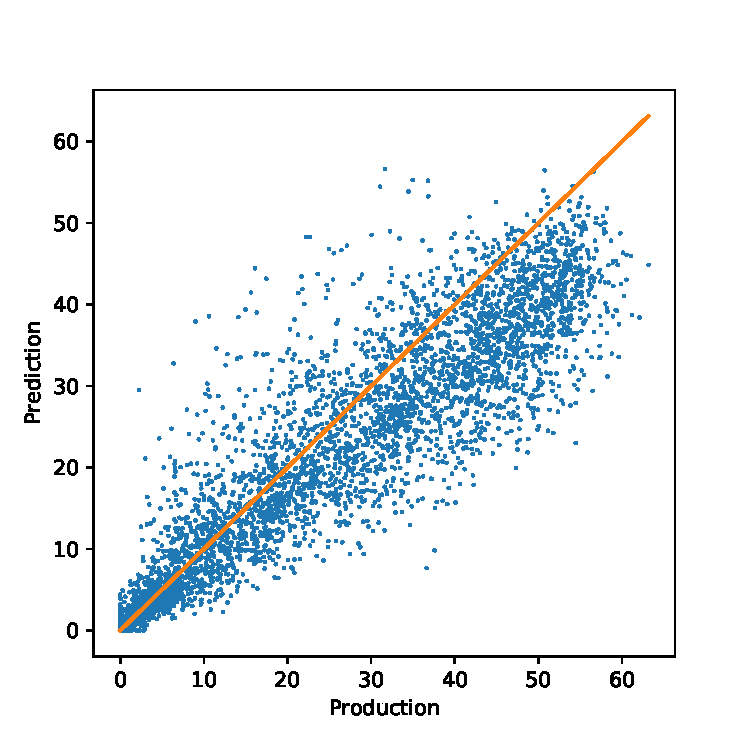
\includegraphics[width=.3 \textwidth, height=.3 \textwidth]{Chapter4/energies/best_ctl_majorca.pdf}
    \label{fig:best_ctl_majorca}}\quad%
    \subfloat[]{%
    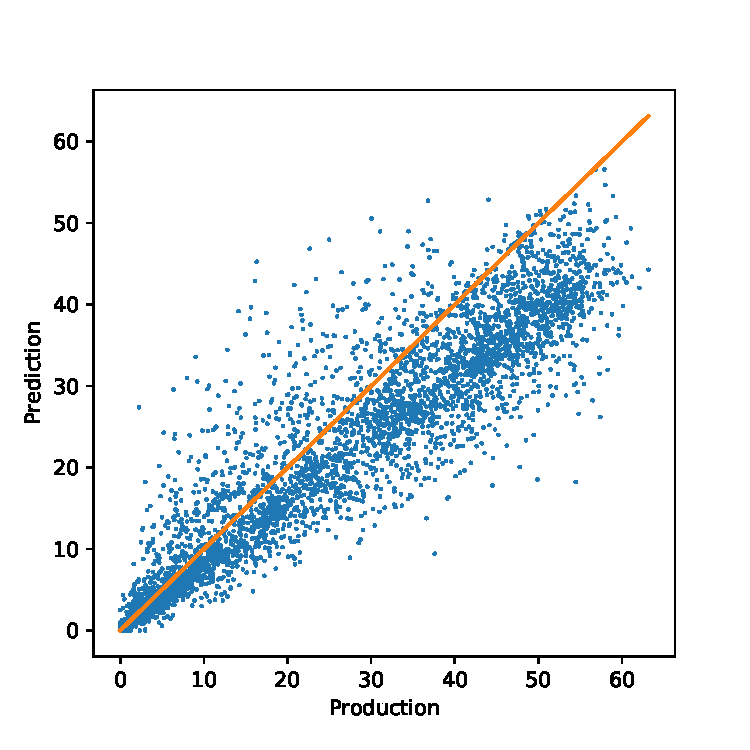
\includegraphics[width=.3 \textwidth, height=.3 \textwidth]{Chapter4/energies/best_itl_majorca.pdf}
    \label{fig:best_itl_majorca}}\quad%
    \subfloat[]{%
    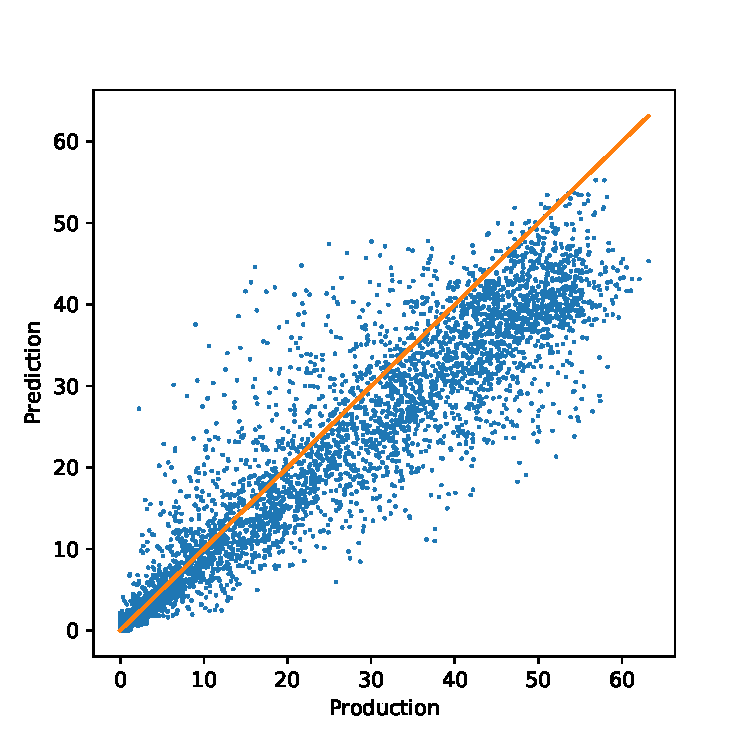
\includegraphics[width=.3 \textwidth, height=.3 \textwidth]{Chapter4/energies/best_mtl_majorca.pdf}
    \label{fig:best_mtl_majorca}}\\
 \caption{\label{fig:majorca_best_plots} Real energy production against prediction made by the best CTL~\protect\subref{fig:best_ctl_majorca}, ITL~\protect\subref{fig:best_itl_majorca}, and MTL~\protect\subref{fig:best_mtl_majorca} models {in} \fcode{majorca} in terms of MAE; the perfect prediction line is shown in orange. The~units of the axis are \mwhu{}.}
\end{figure}

\begin{figure}[H]
    \centering%
    \subfloat[]{%
    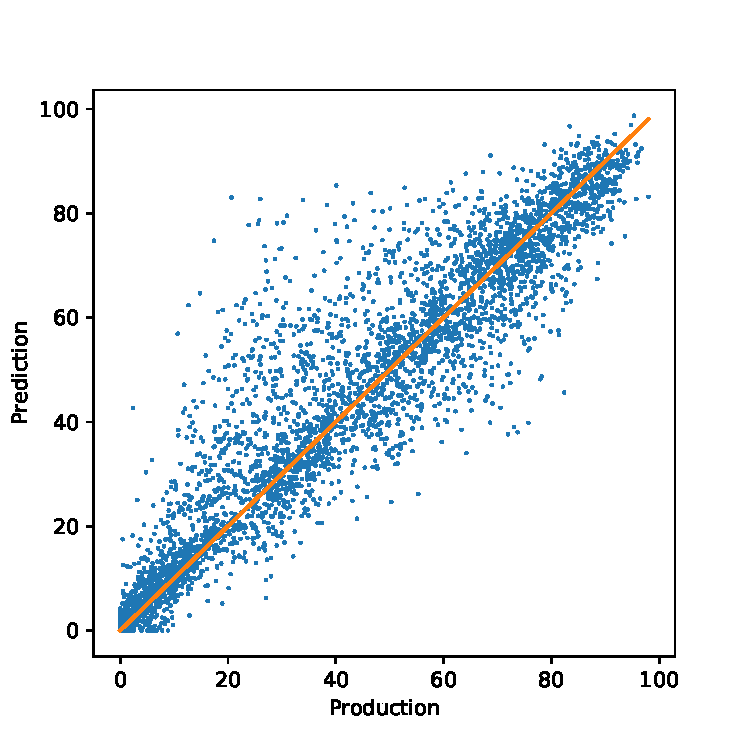
\includegraphics[width=.3 \textwidth, height=.3 \textwidth]{Chapter4/energies/best_ctl_tenerife.pdf}
    \label{fig:best_ctl_tenerife}}\quad%
    \subfloat[]{%
    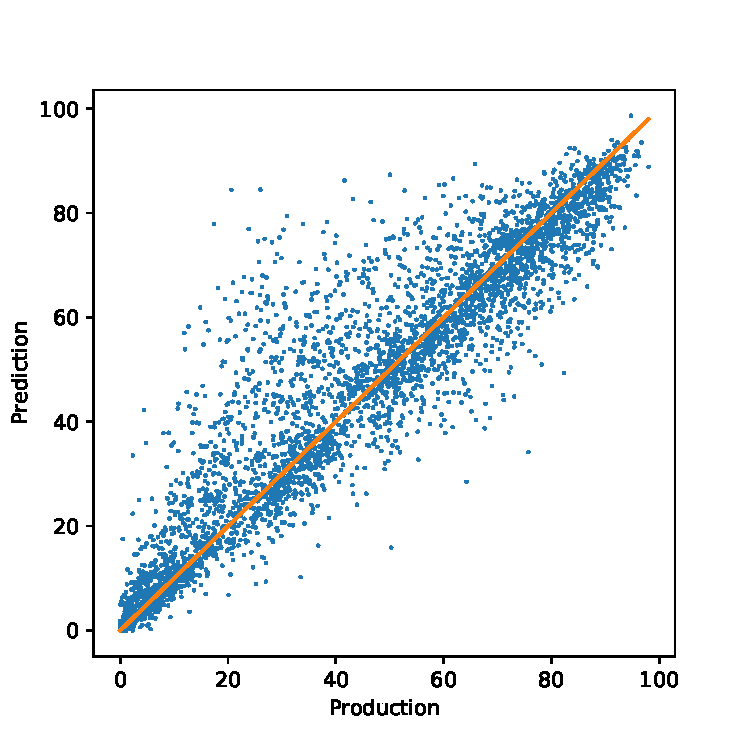
\includegraphics[width=.3 \textwidth, height=.3 \textwidth]{Chapter4/energies/best_itl_tenerife.pdf}
    \label{fig:best_itl_tenerife}}\quad%
    \subfloat[]{%
    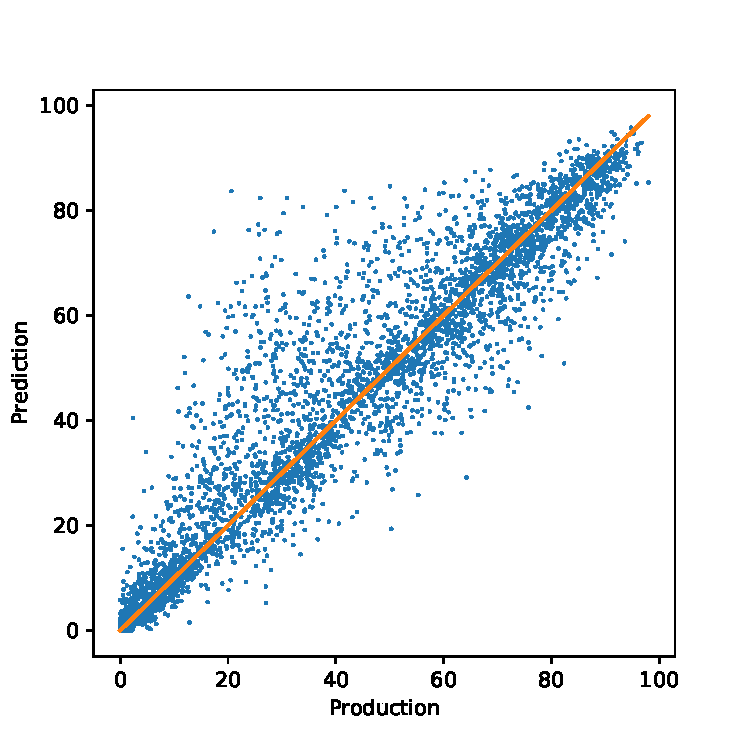
\includegraphics[width=.3 \textwidth, height=.3 \textwidth]{Chapter4/energies/best_mtl_tenerife.pdf}
    \label{fig:best_mtl_tenerife}}\\
 \caption{\label{fig:tenerife_best_plots} Real energy production against prediction made by the best CTL~\protect\subref{fig:best_ctl_tenerife}, ITL~\protect\subref{fig:best_itl_tenerife}, and MTL~\protect\subref{fig:best_mtl_tenerife} models {in} \fcode{tenerife} in terms of MAE; the perfect prediction  line is shown in orange. The~units of the axis are \mwhu{}.}
\end{figure}


%
To get a better understanding of the results we plot the predictions against the target values of the CTL model and the best ITL and MTL ones.
%
In the case of \fdata{majorca}, we plot the predictions \fmod{ctlSVR}, \fmodt{hour}{itlSVR} and \fmodt{season}{mtlSVR} in Figure~\ref{fig:majorca_best_plots}.
From these scatter plots it seems that the CTL approach has a larger deviation in its predictions, while the ITL one has a bias, that is, it systematically underestimates the prediction corresponding to larger values of energy production.
The MTL approach seems to correct, to a certain degree, this bias of the ITL model, while preserving a smaller variance than the CTL one.
%
For \fdata{tenerife} we plot the predictions of \fmod{ctlSVR}, \fmodt{hour}{itlSVR} and \fmodt{hour}{mtlSVR}, which are shown in Figure~\ref{fig:tenerife_best_plots}.
It is more difficult to interpret the plots in this case, although it is possible to highlight that the MTL approach seems less prone to overestimate the production at lower values than either the CTL or ITL models.








\subsection{Wind Energy}

\paragraph*{Data and~Tasks.\\}

\begin{figure}[H]
    \centering%
    \subfloat[]{%
    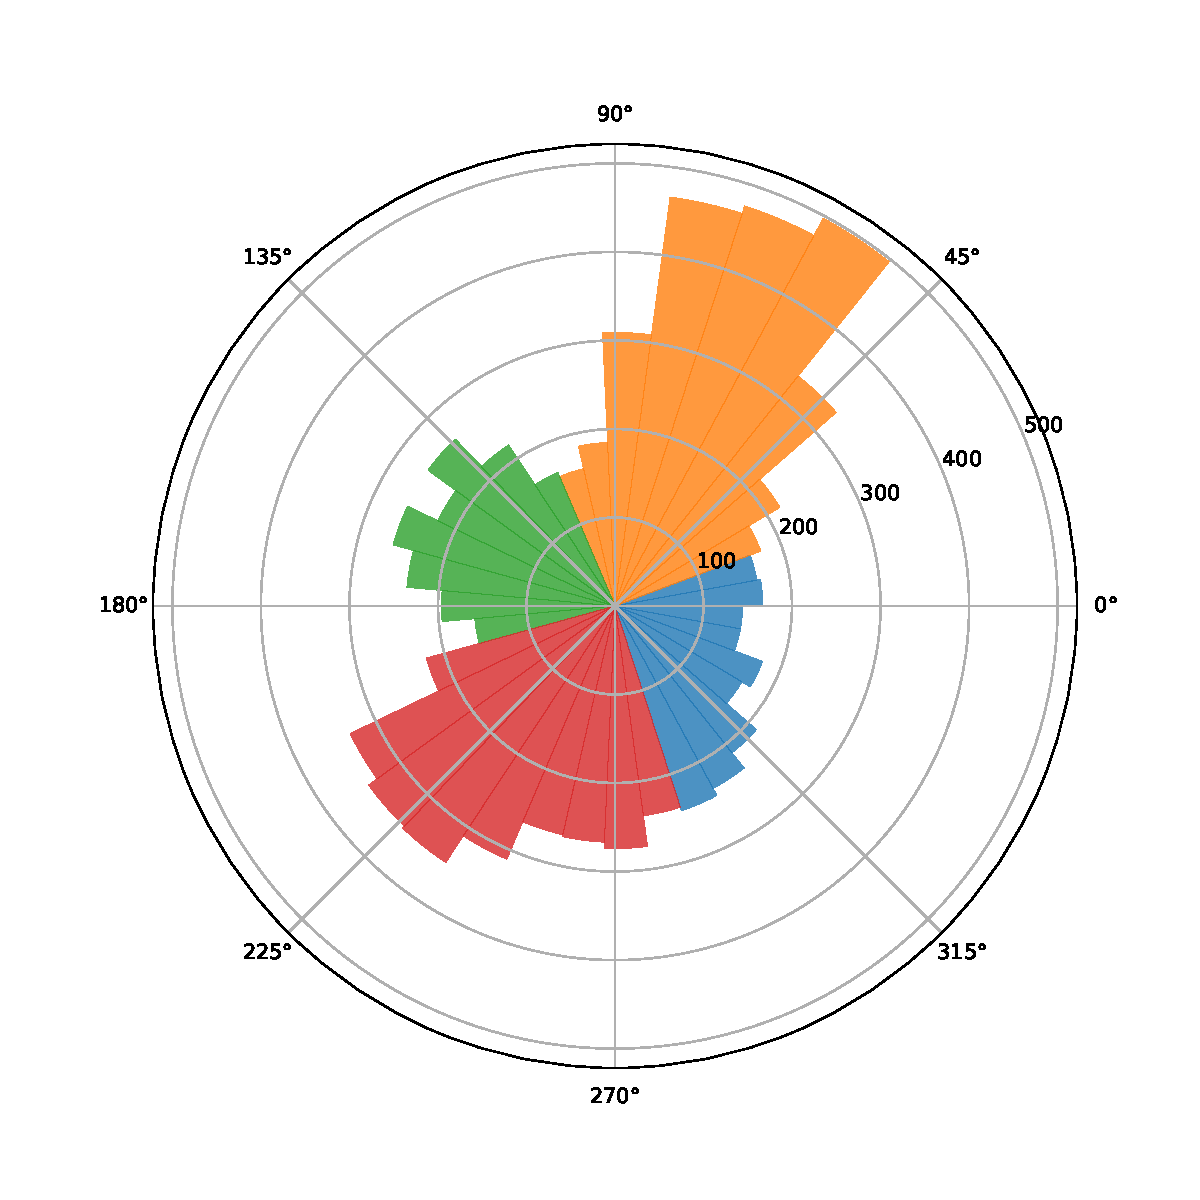
\includegraphics[width=.38 \textwidth]{Chapter4/energies/polarhist_tasks_angle_stv_train.pdf}
    \label{fig:stv_task_angle}}\quad%
    \subfloat[]{%
    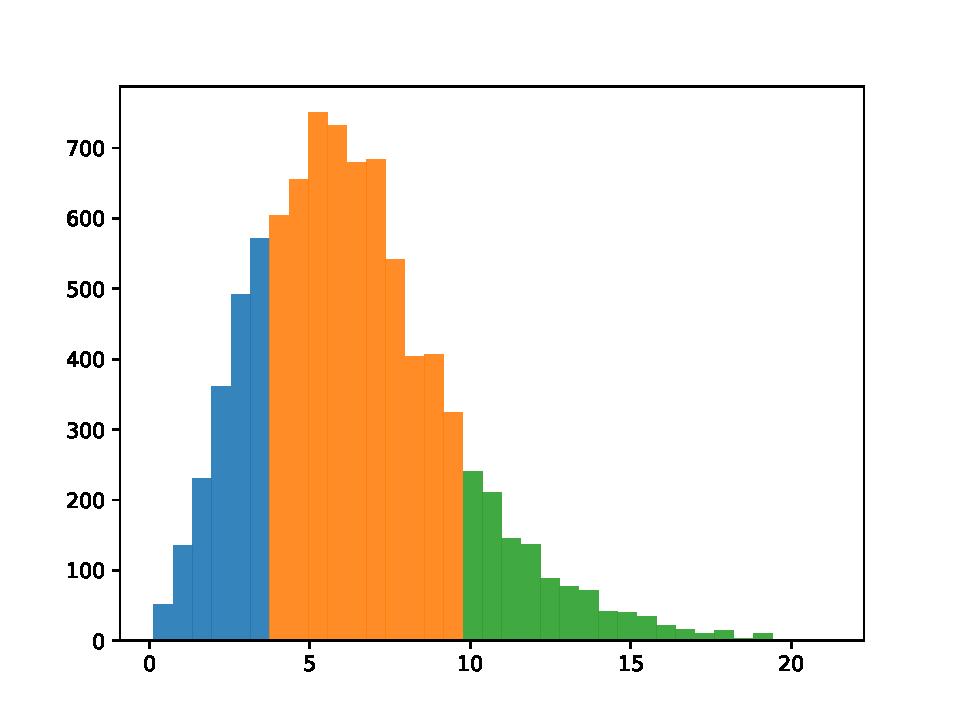
\includegraphics[width=.38 \textwidth]{Chapter4/energies/hist_tasks_velocity_stv_train.pdf}
    \label{fig:stv_task_velocity}}\\
 \caption{\label{fig:wind_task_def} Histograms of wind. ~\protect\subref{fig:stv_task_angle} {Histogram} %Please add figure caption. For example. Figure 4. xxxx (a)xxxx (b)xxxxxx.
  of wind angles derived from NWP data for the year 2016 in Sotavento colored by task \fmod{angle}. ~\protect\subref{fig:stv_task_velocity}  Histogram of wind velocity derived from NWP data for the year 2016 and measured in m/s in Sotavento colored by {task} \fmod{velocity}.}
\end{figure}

 \begin{figure}[H]
   \centering
   \subfloat[]{%
   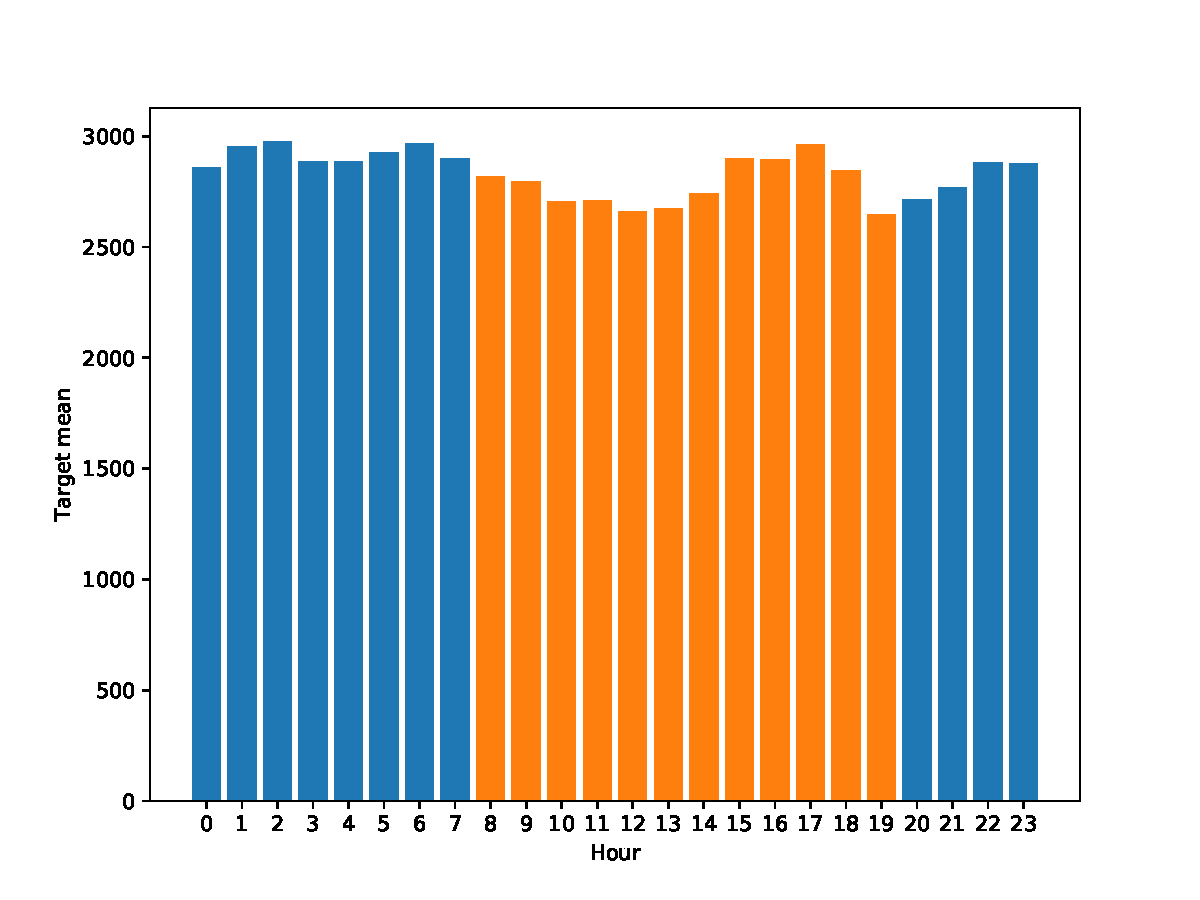
\includegraphics[width=.45 \textwidth]{Chapter4/energies/hist_timeOfDay_stv_train_byHour.pdf}
   \label{fig:hist_timeOfDay_stv_target}}%
\subfloat[]{%
    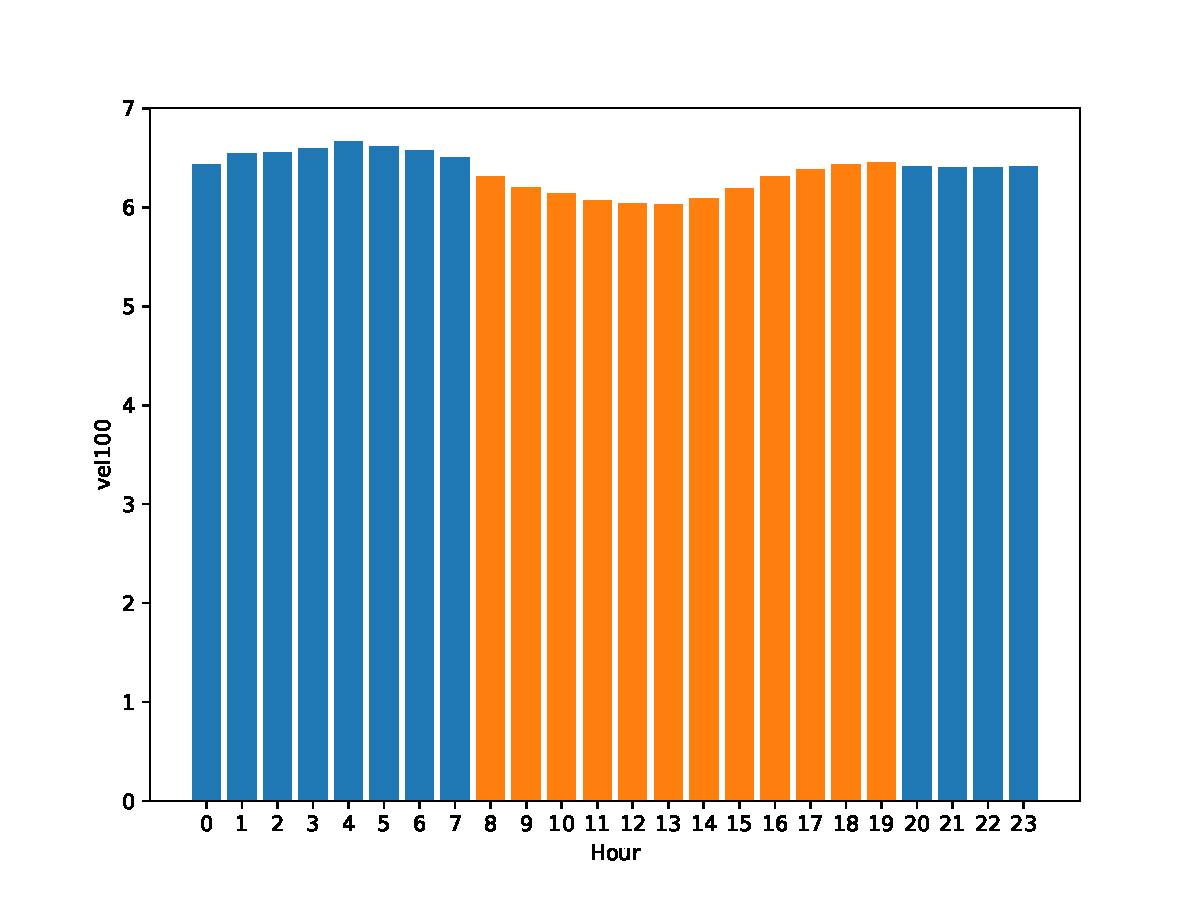
\includegraphics[width=.45 \textwidth]{Chapter4/energies/hist_timeOfDay_stv_vel100_byHour.pdf}
    \label{fig:hist_timeOfDay_stv_vel100}}
% \hspace{\fill}
\caption{\label{fig:wind_task_def_tday} Histograms of wind. ~\protect\subref{fig:hist_timeOfDay_stv_target} {Hourly mean measured} %Please add figure caption. For example. Figure 5. xxxxx (a)xxxxx (b)xxxx. In addition, is it necessary to add explanations of different color cylinders?
 in \si{\kilo{\watt\hour}} of generated energy during the year 2016 in Sotavento colored by {task} \fmod{timeOfDay}. ~\protect\subref{fig:hist_timeOfDay_stv_vel100} Hourly mean of velocity in Sotavento derived from NWP data for the year 2016 and measured in m/s at \SI{100}{\metre} colored by {task} \fmod{timeOfDay}.}
\end{figure}

\begin{figure}[H]
   \centering
   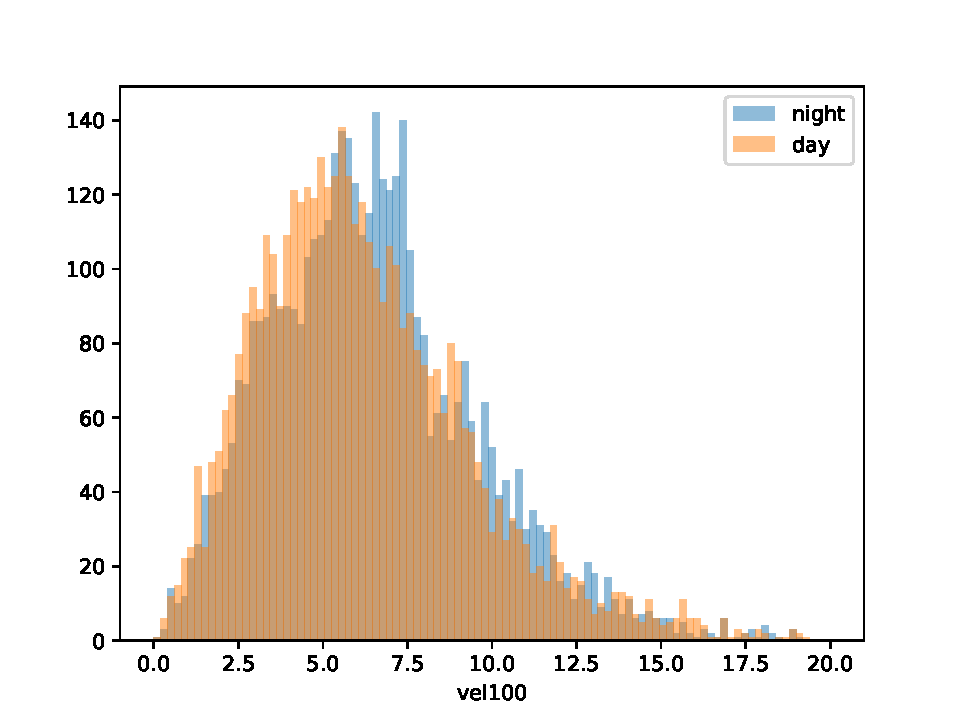
\includegraphics[width=.5\textwidth]{Chapter4/energies/hist_timeOfDay_stv_vel100_normal.pdf}
 \caption{\label{fig:stv_vel100} Histograms of the velocity of wind at 100m derived from NWP data for the year 2016 and measured in m/s during the day and night in Sotavento.
%  \comm{decir para qué año. Hay una cosa que no entiendo: a ojo parece que hay más datos de night que de day, lo que no debería ser. Pero mirando la fig anterior hay 11 horas night-azul- y 13 day naranja. Claramente está mal, pero así las cosas los colores de abajo están al revés}
}
\end{figure}

We want to predict the wind energy production at the Sotavento wind park located in Galicia, Spain. The variables from the NWP that we consider as predictors are:
\begin{itemize}
    \item	Eastward component of the wind at {10 m} %Please remove the font. Same as below
     (\ftt{U10}).
    \item	Northward  component of the wind at {10 m} (\ftt{V10}).
    \item   Module of velocity of the wind at 10 m.
    \item	Eastward  component of the wind at {100 m} (\ftt{U100}).
    \item	Northward component of the wind at {100 m} (\ftt{V100}).
    \item   Module of velocity of the wind at 100 m.
    \item   Surface {Pressure} (\ftt{sp}).
    \item	2 meter {temperature} (\ftt{2t})
\end{itemize}
These variables are collected in a grid, which is approximately centered at the farm, with northeast and southwest coordinates at $(\ang{-9.5}, \ang{44})$ and $(\ang{-6}, \ang{42.25})$, respectively, and a spatial resolution of $\ang{0.125}$.
This results in a grid with $435$ points, that, with the $8$ variables considered at each point, gives a total number of {3480} predictive features.
We scale the energy productions values to $[0, 100]$ using the maximum power installed (\mw{17.56}), which corresponds to the value $100$.
%
Recall that we have three years of data: 2016, 2017 and 2018, which are used as train, validation and test sets.
%
Although there are no obvious task definitions, we consider three different criteria:
\begin{itemize}
    \item \fmod{angle}: Here the wind angle at a height of $100m$ is considered, which is obtained from the \ftt{U100} and \ftt{V100} variables. 
    First, the most frequent angle is estimated, which is $\ang{56}$, and then, we use it as the center of the first quadrant. That is, the patterns that correspond to the first task as those whose wind angle lies between ${11}$ and $\ang{101}$  The other three quadrants, corresponding to a task each, are defined by the remaining sectors of $\ang{90}$.
    The histogram of wind angles, and the defined quadrants in different colors, are shown in Figure~\ref{fig:stv_task_angle}
    \item \fmod{velocity}: Here the wind velocity at a height of $100m$ is considered, which is again obtained from the \ftt{U100} and \ftt{V100} variables. The speed boundaries selected to define three tasks are $4$ and $10$m/s, which, for an ideal generator, are approximately the starting point of wind energy generation and its maximum power plateau, before cut-off speed.   
    In Figure~\ref{fig:stv_task_velocity} the histrogram of velocities is shown with the task regions colored. 
    \item \fmod{timeOfDay}: Here the 24 hours of a day are divided in two 12 hours periods: a day period between 08 and \utc{19}, and~a night one between 20 to \utc{07}.
    In Figures~\ref{fig:hist_timeOfDay_stv_target} and~\ref{fig:hist_timeOfDay_stv_vel100} the hourly average energy production and wind speed are shown, with the hours colored according to the two tasks defined. In Figure~\ref{fig:stv_vel100} the histograms of wind velocity in the night and day periods are shown.
\end{itemize}
%
For these task definitions, it is necessary to perform an analysis of the data, which is done only using the train set, corresponding to 2016.
The tasks in this case are not as clear as that defined for the solar energy. For the \fmod{angle} and \fmod{velocity} definitions some differences across tasks in the histograms can be found, but not definitive ones.
For the \fmod{timeOfDay} definition, the two histograms of Figure~\ref{fig:stv_vel100} look very similar.
Moreover, the boundaries of the tasks are set in a way that is partially arbitrary, and a bad selection of tasks could lead to poor results.


\paragraph*{Experimental~Results.\\}


\begin{table}[H]
    \caption{Test MAEs (left), {MSEs} %Please remove the font in the table. Same in Table 6.
     scores (center), and optimal mixing $\lambda^*$ (right) of the Sotavento wind energy models considered. The~best model errors are shown in~bold.}
    \centering
    \label{table:wind_scores}
    %% \tablesize{} %% You can specify the fontsize here, e.g.,~\tablesize{\footnotesize}. If commented out \small will be used.
    \begin{tabular}{lccc}
    \toprule
    & \fhead{MAE} &  \fhead{MSE} &  \fhead{$\lambda^*$}\\
%    & \fhead{\fcode{stv}}	& \fhead{\fcode{stv}} & \fhead{\fcode{stv}} \\
    \midrule
    \fmod{ctlSVR}                                           &   \fmaxn{6.132} (1) &    90.228 (2) & - \\
    \fmod{(velocity)\_itlSVR}                              &  6.211 (7) &   93.363 (7) & - \\
    \fmod{(velocity)\_mtlSVR}                       &   6.208 (6) &    93.199 (6) & 0 \\
    \fmod{(timeOfDay)\_itlSVR}                             &  6.283 (9) &   93.594 (9) & - \\
    \fmod{(timeOfDay)\_mtlSVR}                      &   \fmaxn{6.132} (1) &    90.228 (2) & 1 \\
    \fmod{(timeOfDay, velocity)\_itlSVR}                 &  6.341 (11) &   97.250 (11) & - \\
    \fmod{(timeOfDay, velocity)\_mtlSVR}          &  6.312 (10) &   94.774 (10) & 0.4 \\
    \fmod{(timeOfDay, angle)\_itlSVR}                    &  6.266 (8) &   93.517 (8) & - \\
    \fmod{(timeOfDay, angle)\_mtlSVR}             &   \fmaxn{6.132} (1) &    90.228 (2) & 1 \\
    \fmod{(timeOfDay, angle, velocity)\_itlSVR}        &  6.410 (12) &  102.031 (12) & - \\
    \fmod{(timeOfDay, angle, velocity)\_mtlSVR} &   \fmaxn{6.132} (1) &    90.228 (2) & 1 \\
    \fmod{(angle)\_itlSVR}                                 &   6.170 (4) &    91.586 (4) & - \\
    \fmod{(angle)\_mtlSVR}                          &   6.135 (2) &    \fmaxn{90.026} (1) & 0.9 \\
    \fmod{(angle, velocity)\_itlSVR}                     &   6.173 (5) &    92.529 (5) & - \\
    \fmod{(angle, velocity)\_mtlSVR}              &   6.168 (3) &    90.990 (3) & 0.7 \\
    \bottomrule
    \end{tabular}
\end{table}



\begin{table}[H]
    \caption{Wilcoxon $p$-values and {corresponding} %Please add explanations of ``—''. In addition, please remove bold if appropritate.
     ranking for absolute (right) and quadratic (left) wind energy errors in~Sotavento. The positions with hyphens correspond to the model ranked first in terms of MAE or MSE, as indicated by its column.}
    \centering
    \label{table:wind_wilcoxon}
    %% \tablesize{} %% You can specify the fontsize here, e.g.,~\tablesize{\footnotesize}. If commented out \small will be used.
    \begin{tabular}{lcc}
    \toprule
    & \fhead{MAE} &  \fhead{MSE}\\
%    & \fhead{\fcode{stv}}	& \fhead{\fcode{stv}} \\
    \midrule
\fmod{ctlSVR}                                           &     ------  {(1)} &    ------   (2)  \\
\fmod{(velocity)\_itlSVR}                              &    0.570  (3) &    0.150  (3)  \\
\fmod{(velocity)\_mtlSVR}                       &    0.356  (3) &    0.466 (3)  \\
\fmod{(timeOfDay)\_itlSVR}                             &    0.195  (4) &    0.258  (4)  \\
\fmod{(timeOfDay)\_mtlSVR}                      &      ------   {(1)} &      ------   (2)  \\
\fmod{(timeOfDay, velocity)\_itlSVR}                 &    0.941  (4) &    0.021  (5)  \\
\fmod{(timeOfDay, velocity)\_mtlSVR}          &    0.428  (4) &    0.650 (4)  \\
\fmod{(timeOfDay, angle)\_itlSVR}                    &    0.000  (4) &    0.015  (4)  \\
\fmod{(timeOfDay, angle)\_mtlSVR}             &      ------   {(1)} &      ------   (2)  \\
\fmod{(timeOfDay, angle, velocity)\_itlSVR}        &    0.090  (4) &    0.024  (6)  \\
\fmod{(timeOfDay, angle, velocity)\_mtlSVR} &   ------  {(1)} &    ------   (2)  \\
\fmod{(angle)\_itlSVR}                                 &    0.855  (3) &    0.644  (3)  \\
\fmod{(angle)\_mtlSVR}                          &    0.035  (2) &   ------  {(1)} \\
\fmod{(angle, velocity)\_itlSVR}                     &    0.253  (3) &    0.465  (3)  \\
\fmod{(angle, velocity)\_mtlSVR}              &    0.018  (3) &    0.001 (3)   \\
\bottomrule
    \end{tabular}
\end{table}

In Table~\ref{table:wind_scores} the MAE and MSE scores are shown, and also the ranking is given in parentheses. 
Unlike the solar energy case, here the CTL approach seems to better suited than using an ITL one. This is also reflected in the selection of $\lambda^*$ values, that are close to $1$, the CTL equivalent case, in the models that get best results, see all the models using $\lambda^*=1$, which are equivalent to \fmod{ctlSVR} but also the cases of \fmodt{angle}{mtlSVR} and \fmodt{angle, velocity}{mtlSVR}, that are second and third using $\lambda^*=0.9$ and $\lambda^*=0.7$.
Those models who put the emphasis on the independent parts, like \fmodt{timeOfDay, velocity}{mtlSVR}, and, of course, the ITL approaches, get worse results.
%
%
As with the solar energy problems, the statistical significance of the results is tested using the Wilcoxon test. As before, using the ranking of Table~\ref{table:wind_scores}, the significance of the difference between one model and its immediate succesor is tested. 
%
In Table~\ref{table:wind_wilcoxon} the $p$-values of these Wilcoxon tests are given, and the statistical significant ranking is shown. Recall that two models have different significant ranking only if the Wilcoxon test hypothesis is refused.
%
The CTL approach obtains the best results, being the best model in terms of MAE and second best in terms of MSE. Nevertheless, the equivalent MTL approaches that use $\lambda^*=1$ trivially tie at first place, these are \fmodt{timeOfDay}{mtlSVR}, \fmodt{timeOfDay, angle}{mtlSVR} and \fmodt{timeOfDay, angle, velocity}{mtlSVR}; while the \fmodt{angle}{mtlSVR} gets the second best MAE score.
When the MSE scores are analyzed, the roles are reversed, the \fmodt{angle}{mtlSVR} gets the best result, and the \fmod{ctlSVR} and the equivalents MTL approaches are second.

%
This advantage of the CTL approach can find its roots on poorly defined tasks, which do not have a strong relation with the energy production. Also, the definition of the tasks is made using the train set, data from year 2016, which may not be useful to the validation or test years.
Nevertheless, the MTL approaches, having the possibility of blending to either CTL or ITL approaches get the best results too.

%
In this wind energy problem, the persistence forecasts, which again predict the energy production the previous day at the same hour, obtain an error of $15.64\%$, which is quite large and represent a $150\%$ increase on the lowest error using SVRs. This is not unusual, since the wind velocity or angle between two different days are not necessarily correlated.
%
With the neural network regressor, the error is a $6.66\%$, which is also greater than any of the models considered.

\begin{figure}[H]
    \centering%
    \subfloat[]{%
    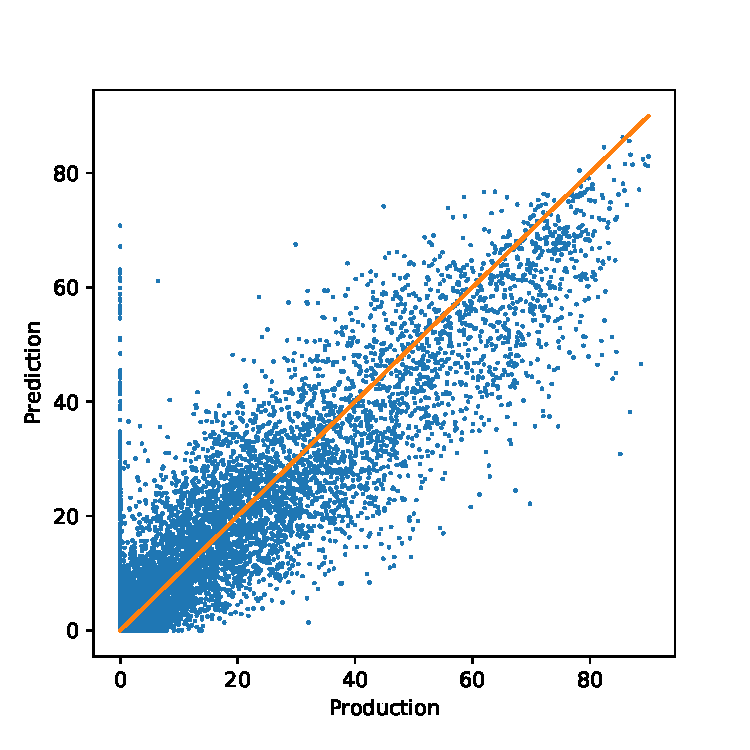
\includegraphics[width=.3 \textwidth, height=.3 \textwidth]{Chapter4/energies/best_ctl_stv.pdf}
    \label{fig:best_ctl_stv}}\quad%
    \subfloat[]{%
    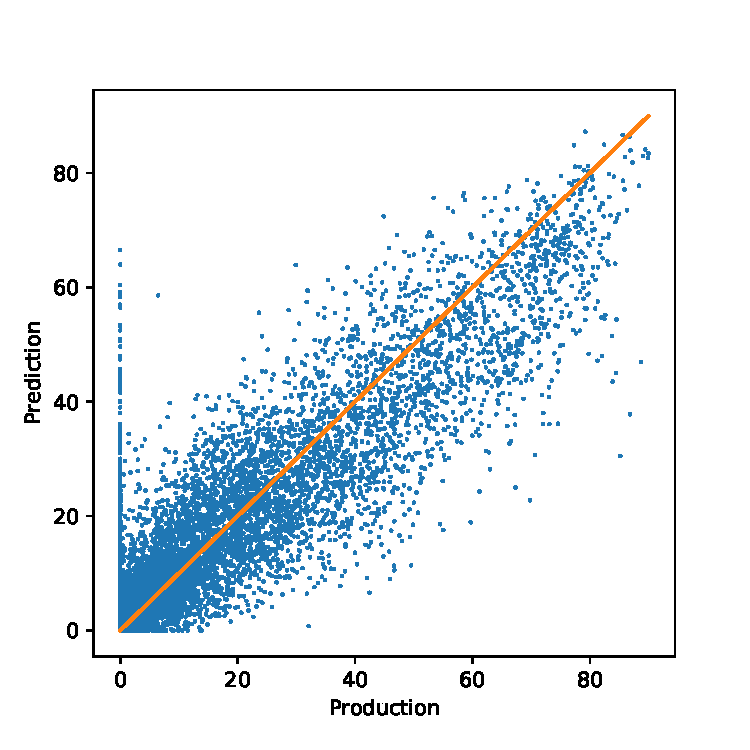
\includegraphics[width=.3 \textwidth, height=.3 \textwidth]{Chapter4/energies/best_itl_stv.pdf}
    \label{fig:best_itl_stv}}\quad%
    \subfloat[]{%
    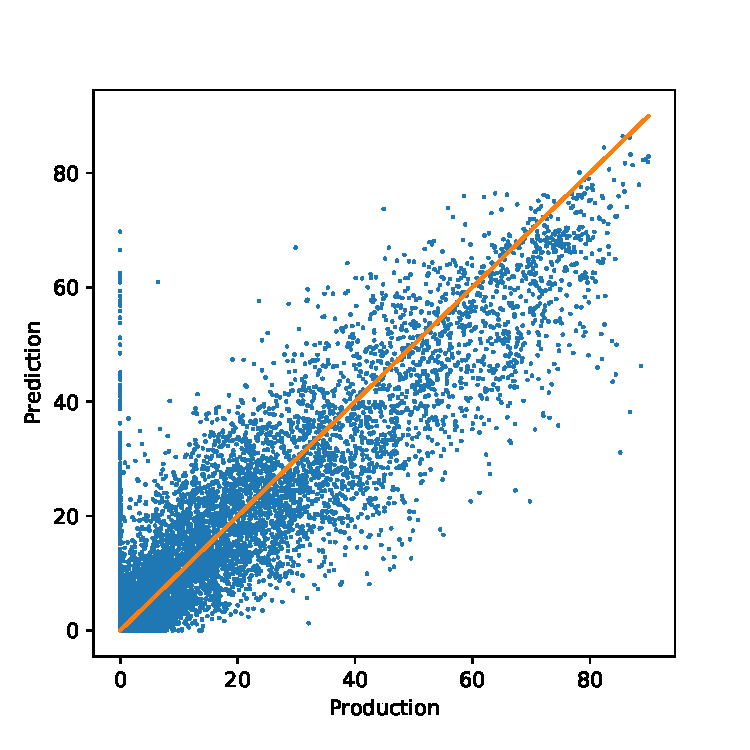
\includegraphics[width=.3 \textwidth, height=.3 \textwidth]{Chapter4/energies/best_mtl_stv.pdf}
    \label{fig:best_mtl_stv}}\\
 \caption{\label{fig:stv_best_plots} Real energy production against prediction made by the best CTL~\protect\subref{fig:best_ctl_stv}, ITL~\protect\subref{fig:best_itl_stv}, and MTL~\protect\subref{fig:best_mtl_stv} models for Sotavento; the perfect prediction line is shown in orange. The~units of the axis are percentages points of the total PV energy~installed.}
 \end{figure}

%
Again, we plot the predictions agains the target values of the CTL model and best ITL,~\fmodt{angle}{itlSVR}, and pure MTL, \fmodt{angle}{mtlSVR} approaches.
The presence of points with zero production is noticeable, but this is relatively frequent in wind energy. It can be caused either by energy curtailments or by maintenance periods of the wind farm.
Also, it is appreciable the frequency of small production values, below \SI{20}{\percent}, which is due to the approximate Weibull distribution of wind speeds, where small speed values have higher frequencies. 
With these considerations, it is difficult to compare the plots and find significant differences in model performance.







% \subsection{Conclusions}

% \paragraph*{old\\}%

% We finally observe that while the wind MAEs in percentage are similar to those in PV, when compared with the energy produced, the~performance of wind models is actually worse.
% In fact, in~Table~\ref{table:comparison} we compare the percentage MAE against the average generated energy as a percentage of installed power.
% As~it can be seen, the~ratio between the percentage MAE and the percentage average energy is about $34.78\%$ for Sotavento, much higher than the $22.50\%$ of Majorca and the $14.92\%$ of~Tenerife.

% \begin{table}[H]
%     \caption{{Comparison}        %Please remove font in the Table
%      of the percentage MAEs with the average energy produced as a percentage of installed~power.}
%     \centering
%     \label{table:comparison}
%     %% \tablesize{} %% You can specify the fontsize here, e.g.,~\tablesize{\footnotesize}. If commented out \small will be used.
%     \begin{tabular}{lccc}
%     \toprule
%  & \fhead{MAE (\%)} & \fhead{Avg. Target (\%)} & \fhead{Ratio} \\
% 	\midrule
% \fdata{majorca} & 6.740 & 29.954 & 22.50 \\
% \fdata{tenerife} & 4.993 & 33.462 & 14.92 \\
% \fdata{sotavento} & 6.186	& 17.784 & 34.78 \\
% \bottomrule
%     \end{tabular}
% \end{table}



\section{Conclusions}\label{sec-conclusions-3}

In this chapter, we have\dots
